\documentclass[a4paper]{article}
\usepackage[svgnames]{xcolor}
\usepackage[a4paper,margin=0.7in]{geometry}
\usepackage[utf8]{inputenc}
\usepackage{url}
\usepackage{hyperref}

\usepackage{enumitem}

% References
\usepackage{natbib}
\bibliographystyle{plainnat}

% Rotate entire figures
\usepackage{rotating}


% Math packages
\usepackage{amsmath,amsfonts,amssymb,amsthm}
\usepackage{mathrsfs}
\usepackage{thmtools}
\usepackage{array}
\usepackage{cleveref}
\usepackage{stmaryrd}
\usepackage{mathpartir}


% Command control packages
\usepackage{ifthen}
\usepackage{ifpdf}

% Listings
\usepackage{listings}
\lstset{
  basicstyle=\ttfamily,
  columns=fullflexible,
  keepspaces=true,
  mathescape
}


% Tikz
\usepackage{tikz}

%%% Comments
% Comments
\newcommand\lau[1]{{\color{purple} \sf \footnotesize {LS: #1}}\\}
\newcommand\dominique[1]{{\color{purple} \sf \footnotesize {DD: #1}}\\}
\newcommand\lars[1]{{\color{purple} \sf \footnotesize {LB: #1}}\\}

%%% Math environments
\declaretheorem[numbered=yes,name=Lemma,qed=$\blacksquare$]{lemma}
\declaretheorem[numbered=yes,name=Theorem,qed=$\blacksquare$]{theorem}
\declaretheorem[numbered=yes,name=Definition,qed=$\blacksquare$]{definition}
\declaretheorem[numbered=yes,name=Specification,qed=$\blacksquare$]{specification}


%%% Math notation
\newcommand{\defeq}{\stackrel{\textit{\tiny{def}}}{=}}
\newcommand{\defbnf}{::=}
\newcommand{\sem}[1]{\left\llbracket #1 \right\rrbracket}
\newcommand{\ssem}[2][\Phi]{\sem{#2}_{\mathrm{src}}(#1)}
\newcommand{\tsem}[2][\Phi]{\sem{#2}_{\mathrm{trg}}(#1)}
\newcommand{\dom}{\mathrm{dom}}
\newcommand{\powerset}[1]{\mathcal{P}(#1)}

\newcommand{\npair}[2][n]{\left(#1,#2\right)}

\newcommand{\nsubeq}[1][n]{\overset{#1}{\subseteq}}
\newcommand{\nsupeq}[1][n]{\overset{#1}{\supseteq}}
\newcommand{\nequal}[1][n]{\overset{#1}{=}}

% Function arrows
\newcommand{\fun}{\rightarrow}
\newcommand{\parfun}{\rightharpoonup}
\newcommand{\monnefun}{\xrightarrow{\textit{\tiny{mon, ne}}}}



% Text
\newcommand{\tand}{\text{ and }}
\newcommand{\tor}{\text{ or }}
\newcommand{\totherwise}{\text{otherwise }}

% Equivalences
\newcommand{\sconeq}{\mathrel{\src{\approx_{\mathrm{ctx}}}}}
\newcommand{\tconeq}{\mathrel{\approx_{\mathrm{ctx}}}}

%%% Logical Relation notation
\newcommand{\typesetlr}[1]{\mathcal{#1}}
\newcommand{\lre}{\typesetlr{E}}
\newcommand{\lrexj}{\typesetlr{E}_{\var{xjmp}}}
\newcommand{\lrk}{\typesetlr{K}}
\newcommand{\lrr}{\typesetlr{R}}
\newcommand{\lro}{\typesetlr{O}}
\newcommand{\lrv}{\typesetlr{V}}
\newcommand{\lrp}{\typesetlr{P}}
\newcommand{\lrm}{\typesetlr{M}}

\newcommand{\stpair}[3][]{
\ifthenelse{\equal{#1}{}}
{\left(\src{#2_S},#3_T\right)}
{\left(\src{#2},#3\right)}}


\newcommand{\memSat}[3][n]{#2 :_{#1}#3}

\newcommand{\World}{\mathrm{World}}
\newcommand{\RegionName}{\mathrm{RegionName}}
\newcommand{\Region}{\mathrm{Region}}
\newcommand{\spatial}{\mathrm{spatial}}
\newcommand{\spatialo}{\mathrm{spatial\_owned}}
\newcommand{\pure}{\mathrm{pure}}
\newcommand{\revoked}{\mathrm{revoked}}
\newcommand{\State}{\mathrm{State}}
\newcommand{\Rels}{\mathrm{Rels}}
\newcommand{\UPred}[1]{\mathrm(#1)}

\newcommand{\future}{\sqsupseteq}
\newcommand{\pub}{\mathrm{pub}}
\newcommand{\privft}{\future^{\priv}}
\newcommand{\pubft}{\future^{\pub}}
\newcommand{\monprivnefun}{\xrightarrow[\text{\tiny{$\privft$}}]{\textit{\tiny{mon, ne}}}}
\newcommand{\monpubnefun}{\xrightarrow[\text{\tiny{$\pubft$}}]{\textit{\tiny{mon, ne}}}}

%%% Regions
\newcommand{\stdreg}[2]{\iota^{\mathrm{std},#2}_{#1}}
\newcommand{\stareg}[2][\stpair{\ms}{\ms}]{\iota^{\mathrm{sta},#2}_{#1}}
\newcommand{\spa}{\mathrm{s}}
\newcommand{\spao}{\mathrm{so}}
\newcommand{\pur}{\mathrm{p}}

%%% Instruction formatting
\newcommand{\sourcecolortext}{blue}
\newcommand{\sourcecolor}{\color{blue}}
\newcommand{\src}[1]{{\sourcecolor #1}}
\newcommand{\targetcolortext}{black}
\newcommand{\targetcolor}[1]{\color{black}}
\newcommand{\trg}[1]{{\targetcolor{} #1}}

\newcommand{\zinstr}[1]{\texttt{#1}}
\newcommand{\oneinstr}[2]{
  \ifthenelse{\equal{#2}{}}
  {\zinstr{#1}}
  {\zinstr{#1} \; #2}
}
\newcommand{\twoinstr}[3]{
  \ifthenelse{\equal{#2#3}{}}
  {\zinstr{#1}}
  {\zinstr{#1} \; #2 \; #3}
}
\newcommand{\threeinstr}[4]{
  \ifthenelse{\equal{#2#3#4}{}}
  {\zinstr{#1}}
  {\zinstr{#1} \; #2 \; #3 \; #4}
}

\newcommand{\fourinstr}[5]{
  \ifthenelse{\equal{#2#3#4#5}{}}
  {\zinstr{#1}}
  {\zinstr{#1} \; #2 \; #3 \; #4 \; #5}
}


%%% Source language
% No arguments
\newcommand{\sfail}{\zinstr{\src{fail}}}
\newcommand{\shalt}{\zinstr{\src{halt}}}
\newcommand{\sreturn}{\zinstr{\src{return}}}

% One argument
\newcommand{\sjmp}[1]{\oneinstr{\src{jmp}}{#1}}
\newcommand{\spush}[1]{\oneinstr{\src{push}}{#1}}
\newcommand{\spop}[1]{\oneinstr{\src{pop}}{#1}}

% Two arguments
\newcommand{\sjnz}[2]{\twoinstr{\src{jnz}}{#1}{#2}}
\newcommand{\sisptr}[2]{\twoinstr{\src{gettype}}{#1}{#2}}
\newcommand{\sgeta}[2]{\twoinstr{\src{geta}}{#1}{#2}}
\newcommand{\sgetb}[2]{\twoinstr{\src{getb}}{#1}{#2}}
\newcommand{\sgete}[2]{\twoinstr{\src{gete}}{#1}{#2}}
\newcommand{\sgetp}[2]{\twoinstr{\src{getp}}{#1}{#2}}
%\newcommand{\sgetloc}[2]{\twoinstr{\src{getloc}}{#1}{#2}}
\newcommand{\sgetlin}[2]{\twoinstr{\src{get}}{#1}{#2}}
\newcommand{\smove}[2]{\twoinstr{\src{move}}{#1}{#2}}
\newcommand{\sstore}[2]{\twoinstr{\src{store}}{#1}{#2}}
\newcommand{\sload}[2]{\twoinstr{\src{load}}{#1}{#2}}
\newcommand{\scca}[2]{\twoinstr{\src{cca}}{#1}{#2}}
\newcommand{\ssload}[2]{\twoinstr{\src{sload}}{#1}{#2}}
\newcommand{\sxjmp}[2]{\twoinstr{\src{xjmp}}{#1}{#2}}
\newcommand{\ssetatob}[2]{\twoinstr{\src{seta2b}}{#1}{#2}}
% scall - special two instruction
\newcommand{\scall}[4][]{  
\ifthenelse{\equal{#3#4}{}}
  {\ensuremath{\zinstr{\src{call}}_{#1}^{#2}}}
  {\ensuremath{\zinstr{\src{call}}_{#1}^{#2} \; #3 \; #4}}
}


% Three arguments
\newcommand{\srestrict}[3]{\threeinstr{\src{restrict}}{#1}{#2}{#3}}
\newcommand{\slt}[3]{\threeinstr{\src{lt}}{#1}{#2}{#3}}
\newcommand{\splus}[3]{\threeinstr{\src{plus}}{#1}{#2}{#3}}
\newcommand{\sminus}[3]{\threeinstr{\src{minus}}{#1}{#2}{#3}}
\newcommand{\scseal}[3]{\threeinstr{\src{cseal}}{#1}{#2}{#3}}
\newcommand{\ssplice}[3]{\threeinstr{\src{splice}}{#1}{#2}{#3}}


% Four arguments
%\newcommand{\ssubseg}[4]{\fourinstr{\src{subseg}}{#1}{#2}{#3}{#4}}
\newcommand{\ssplit}[4]{\fourinstr{\src{split}}{#1}{#2}{#3}{#4}}

%%% Target language
% No arguments
\newcommand{\tfail}{\zinstr{\trg{fail}}}
\newcommand{\thalt}{\zinstr{\trg{halt}}}

% One argument
\newcommand{\tjmp}[1]{\oneinstr{\trg{jmp}}{#1}}

% Two arguments
\newcommand{\tjnz}[2]{\twoinstr{\trg{jnz}}{#1}{#2}}
\newcommand{\tisptr}[2]{\twoinstr{\trg{gettype}}{#1}{#2}}
\newcommand{\tgeta}[2]{\twoinstr{\trg{geta}}{#1}{#2}}
\newcommand{\tgetb}[2]{\twoinstr{\trg{getb}}{#1}{#2}}
\newcommand{\tgete}[2]{\twoinstr{\trg{gete}}{#1}{#2}}
\newcommand{\tgetp}[2]{\twoinstr{\trg{getp}}{#1}{#2}}
%\newcommand{\tgetloc}[2]{\twoinstr{\trg{getloc}}{#1}{#2}}
\newcommand{\tgetlin}[2]{\twoinstr{\trg{getl}}{#1}{#2}}
\newcommand{\tmove}[2]{\twoinstr{\trg{move}}{#1}{#2}}
\newcommand{\tstore}[2]{\twoinstr{\trg{store}}{#1}{#2}}
\newcommand{\tload}[2]{\twoinstr{\trg{load}}{#1}{#2}}
\newcommand{\tcca}[2]{\twoinstr{\trg{cca}}{#1}{#2}}
\newcommand{\txjmp}[2]{\twoinstr{\trg{xjmp}}{#1}{#2}}
\newcommand{\tsetatob}[2]{\twoinstr{\trg{seta2b}}{#1}{#2}}

% Three arguments
\newcommand{\tsplice}[3]{\threeinstr{\trg{splice}}{#1}{#2}{#3}}
\newcommand{\trestrict}[3]{\threeinstr{\trg{restrict}}{#1}{#2}{#3}}
\newcommand{\tlt}[3]{\threeinstr{\trg{lt}}{#1}{#2}{#3}}
\newcommand{\tplus}[3]{\threeinstr{\trg{plus}}{#1}{#2}{#3}}
\newcommand{\tminus}[3]{\threeinstr{\trg{minus}}{#1}{#2}{#3}}
\newcommand{\tcseal}[3]{\threeinstr{\trg{cseal}}{#1}{#2}{#3}}

% Four arguments
%\newcommand{\tsubseg}[4]{\fourinstr{\trg{subseg}}{#1}{#2}{#3}{#4}}
\newcommand{\tsplit}[4]{\fourinstr{\trg{split}}{#1}{#2}{#3}{#4}}

%%% Domains
\newcommand{\plaindom}[1]{\mathrm{#1}}

\newcommand{\nats}{\mathbb{N}}
\newcommand{\ints}{\mathbb{Z}}

%%% Updates
\newcommand{\update}[2]{[#1 \mapsto #2]}
\newcommand{\updReg}[2]{\update{\reg.#1}{#2}}
\newcommand{\updPc}[1]{\Phi\updReg{\pcreg}{#1}}

%%% Source dom
\newcommand{\shareddom}[1]{\mathrm{#1}}
\newcommand{\RegName}{\shareddom{RegisterName}}
\newcommand{\Addr}{\shareddom{Addr}}
\newcommand{\Seal}{\shareddom{Seal}}
\newcommand{\Perm}{\shareddom{Perm}}
\newcommand{\Caps}{\shareddom{Cap}}
\newcommand{\SealableCaps}{\shareddom{SealableCap}}
\newcommand{\Word}{\shareddom{Word}}
\newcommand{\Instr}{\shareddom{Instr}}
\newcommand{\Mem}{\shareddom{Memory}}
\newcommand{\Reg}{\shareddom{RegisterFile}}
\newcommand{\Stk}{\shareddom{Stack}}
\newcommand{\Conf}{\shareddom{Conf}}
\newcommand{\ExecConf}{\shareddom{ExecConf}}
%\newcommand{\Global}{\shareddom{Global}}
\newcommand{\Linear}{\shareddom{Linear}}
\newcommand{\MemSeg}{\shareddom{MemorySegment}}
\newcommand{\StkFrame}{\shareddom{StackFrame}}
\newcommand{\Stack}{\shareddom{Stack}}

\newcommand{\scbnf}{\shareddom{sc}}
\newcommand{\cbnf}{\shareddom{c}}
\newcommand{\permbnf}{\shareddom{perm}}
\newcommand{\addrbnf}{\shareddom{a}}
\newcommand{\basebnf}{\shareddom{base}}
\newcommand{\aendbnf}{\shareddom{end}}
\newcommand{\rbnf}{\shareddom{r}}
%\newcommand{\glbnf}{\shareddom{gl}}
\newcommand{\linbnf}{\shareddom{l}}
\newcommand{\sealbasebnf}{\sigma_\shareddom{base}}
\newcommand{\sealendbnf}{\sigma_\shareddom{end}}

\newcommand{\sstk}{\shareddom{stk}}
\newcommand{\smsstk}{\shareddom{ms_{stk}}}
\newcommand{\sstkframe}{\shareddom{frame}}
\newcommand{\sopc}{\shareddom{opc}}
\newcommand{\sastk}{\shareddom{a_{stk}}}
\newcommand{\perm}{\var{perm}}
%\newcommand{\gl}{\var{g}}
\newcommand{\lin}{\var{l}}
\newcommand{\base}{\shareddom{base}}
\newcommand{\aend}{\shareddom{end}}
\newcommand{\addr}{\shareddom{a}}
\newcommand{\scap}{\shareddom{c}}
\newcommand{\sms}{\shareddom{ms}}

\newcommand{\stkptr}[1]{\mathrm{stack\text{-}ptr}(#1)}
\newcommand{\retptr}{\mathrm{ret\text{-}ptr}}
\newcommand{\retptrd}{\mathrm{ret\text{-}ptr\text{-}data}}
\newcommand{\retptrc}{\mathrm{ret\text{-}ptr\text{-}code}}

\newcommand{\seal}[1]{\shareddom{seal}(#1)}
\newcommand{\sealed}[1]{\shareddom{sealed}(#1)}

\newcommand{\failed}{\mathrm{failed}}
% DOMI: defining a macro named ``undefined'' breaks many latex packages.
%       (this is just another way that LaTeX is broken as a programming language)
% \newcommand{\undefined}{\mathrm{undefined}}
\newcommand{\tundefined}{\mathrm{undefined}}
\newcommand{\halted}{\mathrm{halted}}

%%% Target domain
\newcommand{\targetdom}[1]{\mathrm{#1}}
\newcommand{\tRegName}{\targetdom{RegisterName}}

%%% Programs and contexts
\newcommand{\program}{\mathscr{P}}
\newcommand{\context}{\mathscr{C}}

\newcommand{\plug}[2]{#1[#2]}

%%% Operational semantics
\newcommand{\step}{\rightarrow}
\newcommand{\nstep}[1][n]{\step_{#1}}
\newcommand{\steps}{\step^*}
\newcommand{\diverge}{{\Uparrow}}
\newcommand{\term}[1][-]{{\Downarrow_{#1}}}

%%% Variables
\newcommand{\var}[1]{\mathit{#1}}
\newcommand{\rn}{\var{rn}}
\newcommand{\reg}{\var{reg}}
\newcommand{\mem}{\var{mem}}
\newcommand{\ms}{\var{ms}}
\newcommand{\pc}{\var{pc}}
\newcommand{\stk}{\var{stk}}
\newcommand{\link}{\var{link}}
\newcommand{\stkf}{\stk_{\var{frame}}}
\newcommand{\ret}{\var{ret}}
\newcommand{\data}{\var{data}}
\newcommand{\code}{\var{code}}
\newcommand{\priv}{\var{priv}}
\newcommand{\opc}{\var{opc}}
\newcommand{\odata}{\var{odata}}
\newcommand{\vsc}{\var{sc}}
\newcommand{\cb}{\vsc}
\newcommand{\baddr}{\var{b}}
\newcommand{\eaddr}{\var{e}}
\newcommand{\aaddr}{\var{a}}
\newcommand{\stdrng}{[\baddr,\eaddr]}

%%% Constants
\newcommand{\constant}[1]{\mathrm{#1}}
\newcommand{\calllen}{\constant{call\_len}}
\newcommand{\stkb}{\constant{stk\_base}}

%%% Named registers
\newcommand{\pcreg}{\mathrm{pc}}
\newcommand{\rstk}{\mathrm{r}_\mathrm{stk}}
\newcommand{\rO}{\mathrm{r}_\mathrm{ret}}
\newcommand{\rret}{\rO}
\newcommand{\rretc}{\mathrm{r}_\mathrm{ret code}}
\newcommand{\rretd}{\mathrm{r}_\mathrm{ret data}}
\newcommand{\rdata}{\mathrm{r}_\mathrm{data}}
\newcommand{\rtmp}[1]{\mathrm{r}_\mathrm{t#1}}



%%% locality
%\newcommand{\plainlocality}[1]{\mathrm{#1}}
%\newcommand{\glob}{\plainlocality{global}}
%\newcommand{\local}{\plainlocality{local}}

%%% linearity
\newcommand{\plainlinearity}[1]{\mathrm{#1}}
\newcommand{\linear}{\plainlinearity{linear}}
\newcommand{\normal}{\plainlinearity{normal}}


%%% Permissions
\newcommand{\plainperm}[1]{\textsc{#1}}
%\newcommand{\rwlx}{\plainperm{rwlx}}
\newcommand{\rwx}{\plainperm{rwx}}
\newcommand{\rx}{\plainperm{rx}}
%\newcommand{\rwlxo}{\plainperm{rwlxo}}
%\newcommand{\rwlo}{\plainperm{rwlo}}
%\newcommand{\rwl}{\plainperm{rwl}}
%\newcommand{\rwxo}{\plainperm{rwxo}}
%\newcommand{\rwo}{\plainperm{rwo}}
\newcommand{\rw}{\plainperm{rw}}
%\newcommand{\rxo}{\plainperm{rxo}}
\newcommand{\readonly}{\plainperm{r}}
\newcommand{\ro}{\readonly}
\newcommand{\noperm}{\plainperm{0}}
%\newcommand{\nopermo}{\plainperm{0o}}
%\newcommand{\enter}{\plainperm{e}}
%\newcommand{\entero}{\plainperm{eo}}

%%% Braces
\newcommand{\comp}[1]{[#1]}

%%% Functions
\newcommand{\plainfun}[2]{
  \ifthenelse{\equal{#2}{}}
  {\mathit{#1}}
  {\mathit{#1}(#2)}
}

%\newcommand{\isLoc}[1]{\plainfun{isLocal}{#1}}
%\newcommand{\nonLoc}[1]{\plainfun{nonLocal}{#1}}
%\newcommand{\opaquePerm}[1]{\plainfun{opaquePerm}{#1}}
%\newcommand{\updPcPerm}[1]{\plainfun{updatePcPerm}{#1}}
%\newcommand{\writeLocalAllowed}[1]{\plainfun{writeLocalAllowed}{#1}}
\newcommand{\addressable}[1]{\plainfun{addressable}{#1}}
\newcommand{\callCond}[1]{\plainfun{callCondition}{#1}}
\newcommand{\decInstr}[1]{\plainfun{decodeInstruction}{#1}}
\newcommand{\decPerm}[1]{\plainfun{decodePerm}{#1}}
\newcommand{\encInstr}[1]{\plainfun{encodeInstruction}{#1}}
\newcommand{\encPerm}[1]{\plainfun{encocePerm}{#1}}
\newcommand{\encLin}[1]{\plainfun{encoceLin}{#1}}
\newcommand{\encType}[1]{\plainfun{encodeType}{#1}}
\newcommand{\exec}[1]{\plainfun{executable}{#1}}
\newcommand{\execCond}[1]{\plainfun{executeCondition}{#1}}
\newcommand{\isLinear}[1]{\plainfun{isLinear}{#1}}
\newcommand{\linCons}[1]{\plainfun{linearityConstraint}{#1}}
\newcommand{\noRetStkMs}[1]{\plainfun{noRetStk_{ms}}{#1}}
\newcommand{\noRetStkReg}[1]{\plainfun{noRetStk_{reg}}{#1}}
\newcommand{\nonExec}[1]{\plainfun{nonExecutable}{#1}}
\newcommand{\nonLinear}[1]{\plainfun{nonLinear}{#1}}
\newcommand{\nonZero}[1]{\plainfun{nonZero}{#1}}
\newcommand{\range}[1]{\plainfun{range}{#1}}
\newcommand{\readAllowed}[1]{\plainfun{readAllowed}{#1}}
\newcommand{\readCond}[1]{\plainfun{readCondition}{#1}}
\newcommand{\writeCond}[1]{\plainfun{writeCondition}{#1}}
\newcommand{\sealAss}[1]{\plainfun{sealAssignment}{#1}}
\newcommand{\updPcAddr}[1]{\plainfun{updatePc}{#1}}
\newcommand{\withinBounds}[1]{\plainfun{withinBounds}{#1}}
\newcommand{\writeAllowed}[1]{\plainfun{writeAllowed}{#1}}
\newcommand{\xjumpResult}[3]{\plainfun{xjumpResult}{#1,#2,#3}}


\title{Technical Report}

\begin{document}
\maketitle
\tableofcontents
\section{The two capability machines}
\subsection{Domains}
\label{sec:domains}

% \dominique{7-9-2017: Should we keep local/global and linear/non-linear?  I was thinking just the latter would suffice...}
% \lau{07-09-2017: The local/global mechanism still has some value as it now can be used for the purpose of arguments that cannot be stored by the receiver (if you are willing to ``pay'' the clearing cost). I do, however, not think that it is strictly necessary here to make things work.}
% \lau{12-09-2017: I will remove the local capabilities today for the reasons we have discussed (they add to the complexity and they seem to be of little to no use without a clear memory instruction).}
\[
  \begin{array}{rrcl}
   \addrbnf,\basebnf \in & \Addr & \defeq & \nats \\
    \sealbasebnf, \sigma \in & \Seal & \defeq & \nats \\
    &\Word & \defeq & \ints \uplus \Caps\\
    \permbnf \in& \Perm & \defbnf & \dots \\
    &\linbnf & \defbnf & \linear \mid \normal \\
    &\aendbnf & \in & \Addr \uplus \{\infty \} \\
    &\sealendbnf & \in & \Seal \uplus \{\infty \} \\
    \scbnf \in &\SealableCaps&\defbnf & ((\permbnf,\linbnf),\basebnf,\aendbnf,\addrbnf) \mid \seal{\sealbasebnf,\sealendbnf,\sigma}\\
    & & & {\sourcecolor{} \mid \stkptr{\permbnf,\basebnf,\aendbnf,\addrbnf}}\\ 
    & & & {\sourcecolor{} \; \mid \retptrd(\basebnf,\aendbnf) \mid \retptrc(\basebnf,\aendbnf,\addrbnf)}\\
    \cbnf \in&\Caps& \defbnf &  \scbnf \mid \sealed{\sigma,\scbnf}\\ 
    &\rbnf & \defbnf &\pcreg \mid \rretd \mid \rretc \mid \rstk \mid \rdata \mid \rtmp{1} \mid \rtmp{2} \mid \dots \\
    &\Reg & \defeq & \RegName \fun \Word\\
    &\Mem & \defeq & \Addr \fun \Word \\
    &\MemSeg & \defeq & \Addr \parfun \Word \\
    {\sourcecolor \sstkframe \in} & {\sourcecolor \StkFrame} & {\sourcecolor \defeq} & {\sourcecolor \Addr \times \MemSeg}\\
    \src{\sstk \in}& \src{ \Stack} & \src{ \defeq} & \src{ \StkFrame^*} \\
    \Phi \in & \ExecConf & \defeq & \Mem \times \Reg {\sourcecolor{} \; \times \; \Stack \times \MemSeg }\\
    &\Conf & \defeq & \ExecConf \uplus \{\failed\} \uplus \{\halted\}
  \end{array}
\]
%\lau{06-09-2017: Should seals also have the option to be linear?}
%\lau{13-09-2017: For now I have added linearity to the seals.}
%\lau{15-12-2017: Removed linearity from seal - I could not come up with a single good reason to have it as we have them here.}
\dominique{27-9-2017: I think we should have versions of $\retptrd$ and $\retptrc$ for non-top stack frames and define that invoking them with the current stack pointer will fail.}
\lau{28-09-2017: Why would you like this? If we want to add this, we will have to be careful, because an old code-return-pointer may fit perfectly well with our new data-return-pointer, so in this case it should not fail. We added the seal to the return pointers, so we had some way of figuring out whether two return pointers would actually fit together.}
\dominique{27-9-2017: Likewise, I think we need to have a source-language representation for a pointer into one of the non-top stack frames, as we may need to be able to back-translate adversary code that reads/writes in those.}
\lau{28-09-2017: At the moment, the only part of the stack that is stored in the stack frame is the private part. Specifically it is the part from the base to the current address of the stack pointer \emph{in $r_\stk$}. This means that if someone saves a stack pointer, so it is not included in the call, then they can still use it because that part of the stack was not encapsulated in a stack frame. Makes sense?}
The target language domains are all the non blue parts in the above. The source language domains are the black and blue parts in the above. Further
\begin{itemize}
\item $\linbnf$ defines domain $\Linear$
\item $\scbnf$ defines domain $\SealableCaps$
\item $\cbnf$ defines domain $\Caps$
\item $\rbnf$ defines the finite set $\RegName$. 
\item $\Perm$ is defined as the set of permissions in Figure~\ref{fig:perm-hier}.
\end{itemize}

In the source language, $\src{\Stack}$ is a call stack that contains the data for each call. The call stack consists of a number of $\src{\StkFrame}$'s that contains 1) the old pc and 2) caller's private stack.
\lau{18-12-2017: Stack frame used to contain the address of the old stack pointer. This should be inferable from other information, so it was removed.}

 In both languages, the base address of the stack is known (the stack grows downwards in memory, so the base address marks the end of the stack). In the target language, this will be the base address of some linear capability. The base address can be any address on the machine, but it will have to remain the same during all of execution. We write this constant as
\[
  \stkb
\]


\subsubsection{Useful definitions}
\begin{definition}
  For a capability $c=((\_,\_),\baddr,\eaddr,\_)$ we say it has range $[\baddr,\eaddr]$ and we define
  \[
    \range{c} = [\baddr,\eaddr]
  \]
  Similarly for seals and stack pointers:
  \[
    \range{\seal{\sigma_\baddr,\sigma_\eaddr,\_}} = [\sigma_\baddr,\sigma_\eaddr]
  \]
  and
  \[
    \src{\range{\stkptr{\_,\baddr,\eaddr,\_}} = [\baddr,\eaddr]}
  \]
\end{definition}

\subsection{Syntax}
\label{sec:syntax}
The target machine is a simple capability machine with memory capabilities and sealed capabilities\footnote{In previous work, we used enter capabilities but for this the complexity introduced by mixing writable and executable memory is difficult to handle.} (inspired by CHERI). The syntax of the instructions of the target machine is defined as follows:
\[
\begin{array}{rcl}
n &\in & \ints \\
\com{r} &\in &  \tRegName \\
\com{\rn} &\defbnf &  \com{r} \mid n \\
\com{i} &\defbnf & \tfail \mid \thalt \mid \tjmp{\com{r}} \mid \tjnz{\com{r}}{\com{\rn}} \mid \tisptr{\com{r}}{\com{r}} \mid \tgeta{\com{r}}{\com{r}} \mid \tgetb{\com{r}}{\com{r}} \mid \\
      & &  \tgete{\com{r}}{\com{r}}\mid \tgetp{\com{r}}{\com{r}} \mid \tgetlin{\com{r}}{\com{r}} \mid \tmove{\com{r}}{\com{\rn}} \mid \tstore{\com{r}}{\com{r}} \mid\\
      & &  \tload{\com{r}}{\com{r}} \mid \tcca{\com{r}}{\com{\rn}} \mid \trestrict{\com{r}}{\com{\rn}} \mid \tlt{\com{r}}{\com{\rn}}{\com{\rn}} \mid \\
  & & \tplus{\com{r}}{\com{\rn}}{\com{\rn}} \mid \tminus{\com{r}}{\com{\rn}}{\com{\rn}} \mid \tsetatob{\com{r}} \mid \txjmp{\com{r}}{\com{r}} \mid \tcseal{\com{r}}{\com{r}} \mid \\ 
      & &   \tsplit{\com{r}}{\com{r}}{\com{r}}{\com{\rn}} \mid\tsplice{\com{r}}{\com{r}}{\com{r}} 
\end{array}
\]
$i$ defines the set $\Instr$

%Lau: resolved:
%\dominique{4-12-2017: some instructions need to be able to take an integer rather than a natural, e.g. cca (as used in the implementation of call).}

The source machine is also a capability machine with memory capabilities and sealed capabilities. Unlike the target machine, the source machine has a built in stack along with special stack and return tokens used in place of the actual capabilities. The syntax of the source machine language is as follows:
\[
  \begin{array}{rcl}
    o & \in & \nats \\
    \src{i} & \defbnf &  \com{i} \mid \scall{\offpc,\offsigma}{r}{r}
  \end{array}
\]
There is one syntactic difference between the source language and the target language, namely the target language has an extra instruction in the $\scall{\offpc,\offsigma}{}{}$ instruction (the $o$ refers to the seal it uses, namely the offset in the seals made available by linking). 

The source machine allows for variable length instructions which we utilise for $\scall{\offpc,\offsigma}{}{}$. In other words, when $\scall{\offpc,\offsigma}{}{}$ is decoded, a series of addresses in memory must contain what corresponds to the call instruction (and be within the range of the pc capability). This is described in more detail when we present the decoding function.

\subsection{Permissions}
%\lau{23-03-2017: I am not sure we need the opaque capabilities anymore.} % I am not sure why I did not think the opaque capabilities where necessary, but I have a feeling we talked about this in Leuven and came to the conclusion that they were necessary.
\begin{figure}[!h]
  \centering
  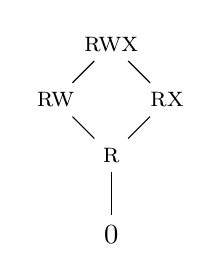
\begin{tikzpicture}[main node/.style={}]
    \node[main node] (rwx) {$\rwx$};
    \node[main node] (rx) [below right of=rwx] {$\rx$};

    \node[main node] (rw) [below left of=rwx,] {$\rw$};
    \node[main node] (r) [below right of=rw] {$\readonly$};
    \node[main node] (0) [below of=r] {$\noperm$};

    \path[every node/.style={font=\sffamily\small}]

    (rw) edge (r)
    (r) edge (0)

    (rwx) edge (rx)

    (rw) edge (rwx)
    (r) edge (rx);
  \end{tikzpicture}

  \caption{Permission hierarchy}
  \label{fig:perm-hier}
\end{figure}
\lau{13-09-2017: Note that most of the discussion below is now captured in Section~\ref{sec:linear-cap}}
\lau{01-09-2017: For now, I will add the linear capabilities such that a linear capability stays linear. It does, however, seem like it would be okay to have linear capabilities become non-linear (I at least don't see anything that would break down completely). One draw back would be that one could ``ruin'' the stack capability by making it non-linear.}
\dominique{7-9-2017: Err... you mean that we could allow non-linear capabilities to be made linear, right?  We definitely do not want to allow the stack or return capability to be made non-linear, as we want to prevent it from being aliased.}
\lau{07-09-2017: I actually did mean linear to non-linear (non-linear to linear does not make sense because the non-linear capability may have aliases). The operation that makes a linear capability non-linear would have to clear said capability. If a linear capability has been made non-linear, then someone who expects a linear capability can observe this difference and behave accordingly, i.e., fail the execution. It will, however, remain an invariant that there are no aliases for linear capabilities.}
\lau{07-09-2017: I had forgotten that return capabilities probably need to be linear. This would call for a ``load from offset'' operation to be able to load an in code stored seal (see the figure I drew about linking/seals).}


We assume functions $\decPerm{}$ and $\encPerm{}$.
\lau{15-09-2017: TODO, write more about these. Should be like in the local cap setting.}

\subsection{Operational Semantics}
The source machine is parameterized with a set of trusted addresses $\ta$. $\ta$ are the only addresses from which the $\scall{}{}{}$ will be interpreted. The source machine represents a virtual intermediate machine which we use to argue well-bracketedness and local state encapsulation. It is not meant to be the machine that the actual code is executed on. Further, it is the well-bracketedness and local state encapsulation of the compiled code, not the context we are concerned with. On the other hand, the target machine is not parameterized with $\ta$ as all the instructions on the target machine is available to the adversary.

\subsubsection{Notes}
Generally:
\begin{itemize}
%\item Opaque capabilities: Only allow locality and permission to be inspected (i.e., no addresses disclosed).
\item Linear capabilities are cleared when they move around in memory.
\end{itemize}

Source language:
\begin{itemize}
\item Variable length instructions that match the length of the compiled instructions
  \begin{itemize}
%  \item Opaque capabilities do not hide the length of a program (especially an issue if we ever hope to have error recovery).
  \item This is needed for correctness. %See subsection~\ref{subsec:capability-opacity} for an example it helps prevent.
  \item It is only used for the call instruction.
  \end{itemize}
% Lau: 18-12-2017: I do not think this is true anymore?
% \item Programs have undefined behavior when passing ret/stk pointers.[\aaddr,\baddr]
\end{itemize}

\dominique{27-09-2017: I think we need to do something about tail calls in the source language?}
\lau{27-09-2017: In what sense? Do you want to allow them (I do not think they are allowed at the moment?)}
\dominique{8-11-2017: Yes, I would like to support them.  I think it would be a strength of our calling convention that we can support them (as I expect we can) and it would be good to demonstrate this.}

Target language:
\begin{itemize}
\item 
\end{itemize}

\subsubsection{Helpful functions, sets, and conventions}

\[
  \pi_\baddr(\vsc) =
  \begin{cases}
    \baddr & \text{if $\vsc = ((\_,\_),\baddr,\_,\_)$} \\ 
    \pi_\baddr(c) & \text{if $\vsc = \sealed{\_,c}$} \\ 
    \src{\baddr} & \src{\text{if $\vsc = \stkptr{\_,\baddr,\_,\_}$}} \\ 
    \src{\baddr} & \src{\text{if $\vsc = \retptrd(\baddr,\_)$}} \\ 
    \src{\baddr} & \src{\text{if $\vsc = \retptrc(\baddr,\_,\_)$}}
  \end{cases}
\]
\[
  \pi_\eaddr(\vsc) =
  \begin{cases}
    \eaddr & \text{if $\vsc = ((\_,\_),\_,\eaddr,\_)$} \\ 
    \pi_\eaddr(c) & \text{if $\vsc = \sealed{\_,c}$} \\ 
    \src{\eaddr} & \src{\text{if $\vsc = \stkptr{\_,\_,\eaddr,\_}$}} \\ 
    \src{\eaddr} & \src{\text{if $\vsc = \retptrd(\_,\eaddr)$}} \\ 
    \src{\eaddr} & \src{\text{if $\vsc = \retptrc(\_,\eaddr,\_)$}}
  \end{cases}
\]

\[
  \pi_\lin(\vsc) = 
  \begin{cases}
    \lin & \text{if $\vsc = ((\_,\_),\_,\eaddr,\_)$} \\ 
    \pi_\lin(c) & \text{if $\vsc = \sealed{\_,c}$} \\ 
    \src{\linear} & \src{\text{if $\vsc = \stkptr{\_,\_,\eaddr,\_}$}} \\ 
    \src{\linear} & \src{\text{if $\vsc = \retptrd(\_,\_)$}} \\ 
    \src{\normal} & \src{\text{if $\vsc = \retptrc(\_,\_,\_)$}}
  \end{cases}
\]

\dominique{4-12-2017: what about $\pi_a$?}
\lau{12-12-2017: I have added them as I needed them in the LR. I have not needed $\pi_a$ yet.}
\[
  \updPcAddr{\Phi} \defeq 
  \begin{cases}
    \Phi\update{\pcreg}{((\perm,\lin),\baddr,\eaddr,\aaddr+1)} & \text{if $\Phi(\pcreg) = ((\perm,\lin),\baddr,\eaddr,\aaddr)$}\\
    \failed & \totherwise
  \end{cases}
\]

\[
  \readAllowed{} \defeq \{ \rwx,\rw,\rx,\ro \}
\]

\[
  \writeAllowed{} \defeq \{ \rwx, \rw \}
\]

\[
  \isLinear{c} \defeq
  \begin{cases}
    \top & 
    \arraycolsep=0pt
    \begin{array}[t]{l}
      c = ((\_,\linear),\_,\_,\_) \tor\\
      c = \sealed{\_,\cb'} \tand \isLinear{\cb'} 
    \end{array}\\
    \src{\top} & 
    \sourcecolor\left.
    \arraycolsep=0pt
    \begin{array}[t]{l}
      c = \stkptr{\_,\_,\_,\_}\\
      c = \retptrd(\_,\_)\\
    \end{array}\right.\\
    \bot & \totherwise
  \end{cases}
\]

We now define 

\[
  \nonLinear{\cb} \defeq \neg \isLinear{\cb}
\]

\[
  \linCons{w} \defeq
  \begin{cases}
    0 & \isLinear{w} \\
    w & \totherwise
  \end{cases}
\]
\[
  \linConsPerm{\perm}{w} \defeq
  \begin{cases}
    \perm \in \writeAllowed{} & \isLinear{w} \\
    \mathrm{true} & \totherwise
  \end{cases}
\]

\[
  \exec{\cb} \defeq 
      \cb = ((\perm, \_), \_, \_, \_) \tand \perm \in \{\rwx,\rx\} 
\]

\[
  \nonExec{\cb} \defeq \neg \exec{\cb}
\]

\[
  \withinBounds{\vsc} \defeq 
  \begin{cases}
    \baddr \leq \aaddr \leq \eaddr & 
    \arraycolsep=0pt
    \begin{array}[t]{l}
      \vsc = ((\_,\_),\baddr,\eaddr,\aaddr) \src{\tor}\\
      \src{\vsc = \stkptr{\_,\baddr,\eaddr,\aaddr}}
    \end{array}\\
    \sigma_\baddr \leq \sigma_\aaddr \leq \sigma_\eaddr & \vsc = \seal{\sigma_\baddr,\sigma_\eaddr,\sigma} \\
    \bot & \totherwise
  \end{cases}
\]

\[
  \nonZero{w} \defeq
  \begin{cases}
    \bot & w \in \ints \tand w = 0 \\
    \top & \totherwise
  \end{cases}
\]


For convenience, we introduce the following notation:
\[
  \begin{array}{rcl}
    \Phi(r) & \defeq & \Phi.\reg(r)
  \end{array}
\]
where $r\in \RegName$.

For $\rn$ which can be a register or an integer, we take
\[
  \Phi(\rn) = n
\]
to mean
\[
  \text{either $n = \rn$ or $n = \Phi.\reg(\rn)$ and in either case $n \in \ints$}
\]


\subsubsection{Step relations}
\paragraph{Decode and encode functions}
We assume functions $\decInstr{} : \Word \fun \Instr$ and $\encInstr{} : \Instr \fun \ints$ where $\Instr$ is the set of target level instructions.

The $\decInstr{}$ function must be surjective and injective for all non-$\tfail$ instructions.
For any $c \in \Caps$, we have that $\decInstr{c} = \tfail$.
The $\encInstr{}$ function must be injective.
Further $\decInstr{}$ must be the left inverse of $\encInstr{}$ that is for all $i \in \Instr$
\[
  \decInstr{}(\encInstr{i}) = i
\]

These functions are used for both the target and source level machine. When we write instructions in places where words are required, we will assume that $\encInstr{}$ is implicit.

\paragraph{Step relation}
The instruction $\scall{\offpc,\offsigma}{}{}$ has length $\calllen$ which means that it does not fit in one memory address. In fact, $\scall{\offpc,\offsigma}{}{}$ should be seen as a different way of interpreting a series of instruction rather than an instruction on its own. We therefore introduce $\scall[0]{\offpc,\offsigma}{r_1}{r_2},\dots,\scall[\calllen-1]{\offpc,\offsigma}{r_1}{r_2}$ as aliases for the instructions that constitute $\scall{\offpc,\offsigma}{r_1}{r_2}$ (see Paragraph~\ref{par:call-impl} for details). We define the following condition that indicates that $\aaddr$ is the first address of a $\scall{\offpc,\offsigma}{r_1}{r_2}$ instruction in the configuration $\Phi$:
\[
  \sourcecolor\left.
    \callCond{\Phi,r_1,r_2,\aaddr} = \left\{
      \begin{array}{l}
        \Phi.\mem(\aaddr) = \scall[0]{\offpc,\offsigma}{r_1}{r_2} \tand\\
        \vdots \\
        \Phi.\mem(\addr+\calllen-1) = \scall[\calllen-1]{\offpc,\offsigma}{r_1}{r_2}
      \end{array}
      \right.
  \right.
\]

We use the following step relation:
\lau{RESOLVED: Add $\ta$ to the source step.}
\lau{RESOLVED: Add $\stkb$ to source term and everything else where it is necessary. Consider how $\stkb$ and $\ta$ can be added without passing around these values in LR and source semantics (solution to parameterize both with it, so they need to be provided only once.)}
\begin{align*}
  \src{\Phi} & \; \src{\step[\src{\ta,\stkb}] \sem{\scall{\offpc,\offsigma}{r_1}{r_2}}(\Phi)} &  &\sourcecolor\left.\arraycolsep=0pt
                                                  \begin{array}[t]{l}
                                                    \text{if }\Phi(\pcreg) 
= ((\perm,\_),\baddr,\eaddr,\aaddr) \tand \\
                                                    \callCond{\Phi,r_1,r_2,\aaddr} \tand\\
                                                    \lbrack \aaddr ,\aaddr + \calllen - 1\rbrack \subseteq \ta \tand \\
                                                    \lbrack\aaddr,\aaddr + \calllen-1\rbrack \subseteq [\baddr,\eaddr] \tand \\
                                                    \exec{\Phi(\pcreg)}
                                                  \end{array}\right.\\
  \Phi & \step[\src{\ta,\stkb}] \sem{\decInstr{\Phi.\mem(\aaddr)}}(\Phi) & &\left.\arraycolsep=0pt
                                                  \begin{array}[t]{l}
                                                    \text{if }\Phi(\pcreg) = ((\perm,\_),\baddr,\eaddr,\aaddr) \tand \\
                                                    \src{(\neg\callCond{\Phi,r_1,r_2,\aaddr} \tor}\\
                                                    \src{\eaddr < \aaddr + \calllen-1) \tand} \\
                                                    \withinBounds{\Phi(\pcreg)} \tand \\
                                                    \exec{\Phi(\pcreg)}
                                                  \end{array}\right.\\
  \Phi& \step[\src{\ta,\stkb}] \failed & & \totherwise
\end{align*}
\dominique{Note: The above does not allow executing code that is on the stack in the source machine, while this is in principle allowed in the target.
This is probably fine if we make sure a stack pointer can never be executable.}

\paragraph{Terminating computations}
We use the following notation to write that a configuration $\Phi$ successfully terminates:
\[
  \Phi\sterm[i]{\src{\ta,\stkb}} \defeq \Phi \nstep[i]{\src{\ta,\stkb}} \halted
\]
if we just know $\Phi$ terminates in some number of steps, then we write
\[
  \Phi\sterm{\src{\ta,\stkb}} \defeq \exists i \ldotp \sterm[i]{\src{\ta,\stkb}}
\]

\paragraph{Call implementation}
\label{par:call-impl}
This paragraph contains the implementation of $\scall{\offpc,\offsigma}{}{}$. That is each of the instructions in the implementation corresponds to $\scall[1]{\offpc,\offsigma}{r_1}{r_2} \dots \scall[\calllen-1]{\offpc,\offsigma}{r_1}{r_2}$, respectively.

%\lau{16-10-2017: Fill this paragraph with $\scall{\offpc,\offsigma}{}{}$ implementation, i.e., the instructions $\scall[1]{\offpc,\offsigma}{r_1}{r_2} \dots \scall[\calllen]{\offpc,\offsigma}{r_1}{r_2}$ is equal to. Add convenience notation like $\update{\mem.a}{\scall{\offpc,\offsigma}{r_1}{r_2}} = \dots$}
\lau{16-10-2017: Implementation of $\scall{\offpc,\offsigma}{}{}$ may need registers for temporary registers - we should update the semantics accordingly.}
\[
  \begin{array}{l}
    \text{// push 42 on the stack (so it is non-empty).}\\
    \tmove{\rtmp{1}}{42}\\
    \tstore{\rstk}{\rtmp{1}}\\
    \tcca{\rstk}{(-1)}\\
    \text{// split the stack at its current address - rstk done.}\\
    \tgeta{\rtmp{1}}{\rstk}\\
    \tsplit{\rstk}{\rretd}{\rstk}{\rtmp{1}}\\
    \text{// load the seal for the return pointer through the pc capability.}\\
    \tmove{\rtmp{1}}{\pcreg}\\
    \tcca{\rtmp{1}}{(\offpc - 5)} \text{ // $\offpc$ is the offset from pc to the location of the seal for this code. \footnote{-5 is the offset from the previous instruction where the $\pcreg$ was moved to $\rtmp{1}$ to the first instruction of the call implementation.}}\\
    \tload{\rtmp{1}}{\rtmp{1}}\\
    
    \tcca{\rtmp{1}}{\offsigma}\text{ // $\offsigma$ is the offset for the seal used by this call.}\\
    \text{// seal the used stack frame as the data part of the return pointer pair.}\\
    \tcseal{\rretd}{\rtmp{1}}\\
    \text{// obtain the code part of the return pointer pair and seal it too.}\\
    \tmove{\rretc}{\pcreg}\\
    \tcca{\rretc}{5} \text{ //magic number is offset to return code}\\
    \tcseal{\rretc}{\rtmp{1}}\\
    \text{// now clear temporary register and jump to the adversary.}\\
    \tmove{\rtmp{1}}{0}\\
    \txjmp{r_1}{r_2}\\
    \text{// the following is the return code}\\
    \text{// check that the stack pointer is the same we handed out.}\\
    \tgetb{\rtmp{1}}{\rstk}\\
    \tminus{\rtmp{1}}{\rtmp{1}}{\stkb} \text{ //$\stkb$ is the stack base constant} \\
    \tmove{\rtmp{2}}{\pcreg}\\
    \tcca{\rtmp{2}}{5} \text{ //magic number is the offset to fail} \\
    \tjnz{\rtmp{2}}{\rtmp{1}} \\
    \tcca{\rtmp{2}}{1} \text{ //magic number is the offset to after fail} \\
    \tjmp{\rtmp{2}} \\
    \tfail \\
    \text{// join our stored private stack frame with the rest of the stack (this also finishes the stack pointer check).}\\
    \tsplice{\rstk}{\rstk}{\rdata} \\
    \text{// pop the magic number 42}\\
    \tcca{\rstk}{1}\\
    \text{// clear temporary registers used}\\
    \tmove{\rtmp{2}}{0}\\
    \text{// continue program after invocation.}
  \end{array}
\]
\dominique{Return code could be simplified if we had jz in addition to jnz.}
% \dominique{It is a bit annoying that we store the stack end address before invocation if we do not use it.
%   I understand this is for ensuring that our private stack frame is not empty, which is important.
%   But why don't we just push a constant then?
%   Also: perhaps we could only do it if the current private stack frame is empty to begin with?
% }
% \dominique{4-12-2017: update: Lau executed the first suggestion (push a constant instead), and convinced me that the last suggestion didn't make sense (only push if the current private stack is empty), because it is then not clear whether or not to pop in the return code.}
The call code does the following:
\begin{itemize}
\item Store 42 (it could be anything) to the stack (this ensures the stack is non-empty), and decrement the pointer according to convention.
\item Get the current address of the stack pointer and split according to it.
\item Retrieve the seal of the program.
\item cca the seal, so the seal to be used is active 
\item seal our private part of the stack capability.
\item Move the pc out of the pc register, adjust it to point to the first address of the return code, and seal it.
\item clear the temporary register.
\item cross jump to the two specified registers.
\item Upon return:
  \begin{itemize}
  \item get the base of the stack and check that it matches up with the global base of the stack.If not, fail.
  \item splice the returned stack pointer and the stack pointer for our private stack.
  \item adjust stack pointer to first empty address (the address with the end address is considered free)  
  \item clear the temporary registers. (Note that $\rtmp{1}$ is not cleared with 0 as it already contains 0 after the $\stkb$ check. If it didn't contain 0, then the execution would have failed.)

  \end{itemize}
\end{itemize}

For convenience, we will add the convention that the memory update $\update{\mem.a}{\scall{\offpc,\offsigma}{r_1}{r_2}}$ corresponds to
\[
  \begin{array}{l}
    \update{\mem.a}{\scall[0]{\offpc,\offsigma}{r_1}{r_2}}\\
    \update{\mem.a+1}{\scall[1]{\offpc,\offsigma}{r_1}{r_2}}\\
    \dots\\
    \update{\mem.a+\calllen-1}{\scall[\calllen-1]{\offpc,\offsigma}{r_1}{r_2}}\\
  \end{array}
\]

\subsubsection{Instruction Interpretation}
We have unified the two languages in the below definitions. Everything written in black is common for both source and target language. Everything written in \src{blue} is specific to the source language.

\noindent\textbf{fail and halt}\\
\begin{align*}
  \sem{\tfail}(\Phi) = & \; \failed \\
  \sem{\thalt}(\Phi) = & \; \halted
\end{align*}

\noindent\textbf{jmp and jnz}\\
\begin{align*}
  \sem{\tjmp{r}}(\Phi) = &  
                     \begin{cases}
                       \Phi\updReg{r}{w}\updReg{\pcreg}{\Phi(r)} & w = \linCons{\Phi(r)}
                     \end{cases}
\end{align*}

\begin{align*}
  \sem{\tjnz{r}{\rn}}(\Phi) = &       
                             \begin{cases}
                               \arraycolsep=0pt
                               \begin{array}[t]{rl}
                                 \Phi&\updReg{r}{w}\\
                                     &\updReg{\pcreg}{\Phi(r)}
                               \end{array} 
                                              & w = \linCons{\Phi(r)} \tand \nonZero{\Phi(\rn)}\\
                               \updPcAddr{\Phi} & \totherwise
                             \end{cases}
\end{align*}

\noindent\textbf{gettype}\\
In the definitions of the semantics below, we use a function $\encType{} : \Word \rightarrow \ints$. This is an encoding function for which the specific implementation does not matter. As the words of the two machines differ, we really need two functions which we call $\encType{}_{\var{src}}$ and $\encType{}_{\var{trg}}$. These two functions need to be related in the following way:
% Lau: 19-12-2017: Resolved the belove by adding the conditions.
%\lau{14-09-2017: Insert the relation. My impression is that the the words specific to the source machine should have the same "type" as their implementation at the source level (I am not sure this is the case - maybe it is okay to just relate the values returned by the special words to the ones returned when used with the implementation). }
%\dominique{20-9-2017: I also think gettype for source-specific words should produce the same result than gettype for their implementation.}
\begin{itemize}
\item $\encType{}(((\_,\_),\_,\_,\_))$, $\encType{}(\seal{\_,\_,\_})$, $\encType{}(\sealed{\_,\_})$, and $\encType{}(i)$ where $i\in\ints$ are all distinct.
\item For all $w \in \SealableCaps$ (only the words on the target machine), $\encType{}_{\var{trg}}(w) = \encType{}_{\var{src}}(w)$.
\item Finally, 
\[
\encType{}_{\var{src}}(\src{\stkptr{\_,\_,\_,\_}}) = \encType{}_{\var{trg}}(((\_,\_),\_,\_,\_))
\]
 and 
\[
\encType{}_{\var{src}}(\src{\retptrd(\_,\_)}) = \encType{}_{\var{src}}(\src{\retptrc(\_,\_,\_)}) = \encType{}_{\var{trg}}(((\_,\_),\_,\_,\_))
\]
\end{itemize}
In English this means that each type of word is represented by a distinct value and that the tokens on the source machine has the type of the capability they represent on the target machine.
\begin{align*}
  \sem{\tisptr{r_1}{r_2}}(\Phi) = & \; \updPcAddr{}(\Phi\updReg{r_1}{\encType{\Phi(r_2)}})
\end{align*}


\noindent\textbf{geta, getb, gete, getp, and getl}\\
We assume functions to encode and decode permissions as well as a function to encode linearity. The functions are used implicitly when a permission or linearity is used in a place where they need to be a word.
%\lau{14-09-2017: Write more about this (types and assumptions)}

Specifically for the permission function, $\encPerm{} : \Perm \fun \ints$ and $\decPerm{} : \ints \fun \Perm $ encodes and decodes permissions, respectively. Where $\decPerm{}$ is the left inverse of $\encPerm{}$, $\encPerm{}$ is injective and for all $\perm \in \Perm$ $\encPerm{\perm} \neq -1$ (as this is used as an error value). $\decPerm{}$ is surjective.

For the linearity encoding, we make similar assumptions: $\encLin{} : \Linear \fun \ints$ encodes linearity. $\encLin{}$ is injective and for all $\lin \in \Linear$ $\encPerm{\lin} \neq -1$ (as this is used as an error value). As a capabilities linearity stays the same, we do not need a decoding function for linearity.
\begin{align*}
  \sem{\tgeta{r_1}{r_2}}(\Phi) = & 
                                   \begin{cases}
                                     \updPcAddr{\Phi\updReg{r_1}{\aaddr}} & 
                                     \arraycolsep=0pt
                                     \begin{array}[t]{l}
                                       \Phi(r_2) = ((\_,\_),\_,\_,\aaddr) \\
                                       \quad \tor \Phi(r_2) = \seal{\_,\_,\aaddr} \\ 
                                       \quad \src{\tor \Phi(r_2) = \stkptr{\_,\_,\_,\aaddr} } \\
                                     \end{array} \\
                                     \updPcAddr{\Phi\updReg{r_1}{-1}} & \totherwise
                                   \end{cases}
\end{align*}

\begin{align*}
  \sem{\tgetb{r_1}{r_2}}(\Phi) = & 
                                   \begin{cases}
                                     \updPcAddr{\Phi\updReg{r_1}{\baddr}} & 
                                     \arraycolsep=0pt
                                     \begin{array}[t]{l}
                                       \Phi(r_2) = ((\_,\_),\baddr,\_,\_) \\
                                       \quad \tor \Phi(r_2) = \seal{\baddr,\_,\_} \\
                                       \quad \src{\tor \Phi(r_2) = \stkptr{\_,\baddr,\_,\_} } \\
                                     \end{array} \\
                                     \updPcAddr{\Phi\updReg{r_1}{-1}} & \totherwise
                                   \end{cases}
\end{align*}

\begin{align*}
  \sem{\tgete{r_1}{r_2}}(\Phi) = & 
                                   \begin{cases}
                                     \updPcAddr{\Phi\updReg{r_1}{\eaddr}} & 
                                     \arraycolsep=0pt
                                     \begin{array}[t]{l}
                                       \Phi(r_2) = ((\_,\_),\_,\eaddr,\_) \\
                                       \quad \tor \Phi(r_2) = \seal{\_,\eaddr,\_} \\
                                       \quad \src{\tor \Phi(r_2) = \stkptr{\_,\_,\eaddr,\_} } \\
                                     \end{array} \\
                                     \updPcAddr{\Phi\updReg{r_1}{-1}} & \totherwise
                                   \end{cases}
\end{align*}
\lau{15-09-2017: Should gete and getb do something for seals?}
\dominique{4-12-2017: doesn't matter, I think.}

\begin{align*}
  \sem{\tgetp{r_1}{r_2}}(\Phi) = & 
                                   \begin{cases}
                                     \updPcAddr{\Phi\updReg{r_1}{\perm}} & 
                                     \arraycolsep=0pt
                                     \begin{array}[t]{l}
                                       \Phi(r_2) = ((\perm,\_),\_,\_,\_) \\
                                       \quad \src{\tor \Phi(r_2) = \stkptr{\perm,\_,\_,\_} } \\
                                     \end{array} \\
                                     \updPcAddr{\Phi\updReg{r_1}{-1}} & \totherwise
                                   \end{cases}
\end{align*}

\begin{align*}
  \sem{\tgetlin{r_1}{r_2}}(\Phi) = & 
                                   \begin{cases}
                                     \updPcAddr{\Phi\updReg{r_1}{\linear}} & 
                                     \arraycolsep=0pt
                                     \begin{array}[t]{l}
                                       \isLinear{\Phi(r_2)}
                                     \end{array} \\
                                     \updPcAddr{\Phi\updReg{r_1}{\normal}} & \nonLinear{\Phi(r_2)}
                                   \end{cases}
\end{align*}
\lau{19-12-2017: Resolved the comments below. Seals are all normal and we allow linearity of sealed capabilities to be retrieved as it is observable anyway.}
\lau{15-09-2017: Should getl do something for seals?}
\dominique{4-12-2017: doesn't matter, I think.}
\lau{15-09-2017: Do we want to allow getl and getp to work on sealed capabilities?}
\dominique{Linearity of sealed caps is already observable anyway, so no point in hiding it.  Permissions of the sealed capability should be hidden, I think, mostly out of conservativity (hide as much as possible!).}\\
\dominique{4-12-2017: Couldn't the definitions above use $\pi_b$, $\pi_e$, $\pi_l$ and $\pi_a$ and $\pi_p$ (the latter two to be added) ?}
\lau{12-12-2017: $\pi_\_$ also projects from sealed capabilities, so the case of sealed capabilities would have to be explicitly excluded (with getl as the exception).}


\noindent\textbf{move}\\
\begin{align*}
  \sem{\tmove{r}{\rn}}(\Phi) = & 
                              \begin{cases}
                                \updPcAddr{\Phi\updReg{r}{\rn}} & \rn \in \ints \\
                                \updPcAddr{\Phi\updReg{\rn}{w}\updReg{r}{\Phi(\rn)}} & w = \linCons{\Phi(\rn)}
                              \end{cases}
\end{align*}
(Notice that in the case where we are moving a linear capability and $r = \rn$ the order of the updates matter.)

\noindent\textbf{store}\\
\begin{align*}
  \sem{\tstore{r_1}{r_2}}(\Phi) = &
                                    \begin{cases}
                                      \updPcAddr{}\left(
                                        \arraycolsep=0pt
                                        \begin{array}{rl}
                                          \Phi&\updReg{r_2}{w_2}\\
                                              &\update{\mem.a}{\Phi(r_2)}
                                        \end{array}
\right) & 
                                      \arraycolsep=0pt
                                      \begin{array}[t]{l}
                                        \Phi(r_1) = ((\perm,\lin),\baddr,\eaddr,\aaddr) \tand \\
                                        \perm \in \writeAllowed{} \tand\\
                                        \withinBounds{\Phi(r_1)} \tand \\
                                        w_2 = \linCons{\Phi(r_2)}
                                      \end{array}
                                      \\
                                      \sourcecolor\left.
                                      \updPcAddr{}\left(
                                      \arraycolsep=0pt
                                      \begin{array}{rl}
                                        \Phi&\updReg{r_2}{w_2}\\
                                            &\update{\ms_\stk.a}{\Phi(r_2)}
                                      \end{array}
                                      \right) \right.& 
                                      \sourcecolor\left.
                                      \arraycolsep=0pt
                                      \begin{array}[t]{l}
                                        \Phi(r_1) = \stkptr{\perm,\baddr,\eaddr,\aaddr} \tand \\
                                        \perm \in \writeAllowed{} \tand \\
                                        \withinBounds{\Phi(r_1)} \tand \\
                                        \aaddr \in \dom(\Phi.\ms_\stk) \tand \\ % Lau: this condition seems odd as there should never be a capability for a piece of memory that is unreachable.
                                        w_2 = \linCons{\Phi(r_2)}
                                      \end{array}\right.\\
                                      \failed & \totherwise
                                    \end{cases}
\end{align*}


\noindent\textbf{load}\\
\begin{align*}
  \sem{\tload{r_1}{r_2}}(\Phi) = & 
                                  \begin{cases}
                                    \updPcAddr{}\left(
                                      \arraycolsep=0pt
                                      \begin{array}{rl}
                                        \Phi&\update{\mem.a}{w_2}\\
                                            &\updReg{r_1}{w}
                                      \end{array}\right)& 
                                    \arraycolsep=0pt
                                    \begin{array}[t]{l}
                                      \Phi(r_2) = ((\perm,\lin),\baddr,\eaddr,\aaddr) \tand \\
                                      \perm \in \readAllowed{} \tand\\
                                      \withinBounds{\Phi(r_2)} \tand \\
                                      w = \Phi.\mem(a) \tand \\
                                      w_2 = \linCons{w} \tand
                                      \linConsPerm{\perm}{w}
                                    \end{array}
                                    \\
                                    \sourcecolor\left.
                                    \updPcAddr{}\left(
                                      \arraycolsep=0pt
                                      \begin{array}{rl}
                                        \Phi& \update{\ms_\stk.a}{w_2}\\
                                            &\updReg{r_1}{w}
                                      \end{array}\right)\right.
                                    & 
                                    \sourcecolor\left.
                                    \arraycolsep=0pt
                                    \begin{array}[t]{l}
                                      \Phi(r_2) = \stkptr{\perm,\baddr,\eaddr,\aaddr} \tand \\
                                      \perm \in \readAllowed{} \tand \\
                                      \withinBounds{\Phi(r_2)} \tand \\
                                      \aaddr \in \dom(\Phi.\ms_\stk) \tand \\ % Lau: this condition seems odd as there should never be a capability for a piece of memory that is unreachable.
                                      w = \Phi.\ms_\stk(a) \tand \\
                                      w_2 = \linCons{w} \tand
                                      \linConsPerm{\perm}{w}
                                    \end{array}\right.
                                    \\
                                    \failed & \totherwise                                    
                                  \end{cases}
\end{align*} 
\dominique{9-3-2018: $\linCons$ should only be allowed to modify the memory if the capability has write permission!}

\noindent\textbf{cca}\\
% The following comment has been resolved by implementing the suggestion.
% \dominique{4-12-2017: The phrase $\text{either $n = \rn$ or $n = \Phi.\reg(\rn)$ and in either case $n \in \ints$ and}$ is repeated a lot in the semantics. Perhaps define an abbreviation as $\Phi(\rn) = n$?}
\emph{Change Current Address}
\\\lau{15-09-2017: This is the old lea. I changed the name, so it actually reflects what the instruction does. We might also want to add a real lea at some point.}
\begin{align*}
  \sem{\tcca{r}{\rn}}(\Phi) = & 
                                  \begin{cases}
                                    \updPcAddr{\Phi\updReg{r}{c}} &  
                                    \arraycolsep=0pt
                                    \begin{array}[t]{l}
                                      \Phi(\rn) = n \tand \\
                                      \Phi(r) = ((\perm,\lin),\baddr,\eaddr,\aaddr) \tand \\
                                      c = ((\perm,\lin),\baddr,\eaddr,\aaddr + n)
                                    \end{array}
                                    \\
                                    \updPcAddr{\Phi\updReg{r}{s}} &  
                                    \arraycolsep=0pt
                                    \begin{array}[t]{l}
                                      \Phi(\rn) = n \tand \\
                                      \Phi(r) = \seal{\sigma_\baddr,\sigma_\eaddr,\sigma} \tand \\
                                      s = \seal{\sigma_\baddr,\sigma_\eaddr,\sigma + n}
                                    \end{array}
                                    \\
                                    \src{\updPcAddr{\Phi\updReg{r}{c}}} &  
                                    \sourcecolor\left.
                                    \arraycolsep=0pt
                                    \begin{array}[t]{l}
                                      \Phi(\rn) = n\tand \\
                                      \Phi(r) = \stkptr{\perm,\baddr,\eaddr,\aaddr} \tand \\
                                      c = \stkptr{\perm,\baddr,\eaddr,\aaddr + n}
                                    \end{array}\right.
                                    \\
                                    \failed & \totherwise
                                  \end{cases}
\end{align*}

\noindent\textbf{restrict}\\
This instruction uses the $\decPerm{}$ function.
\begin{align*}
  \sem{\trestrict{r_1}{\rn}}(\Phi) = &
                                      \begin{cases}
                                        \updPcAddr{}\left(
                                          \arraycolsep=0pt
                                          \begin{array}{rl}
                                          \Phi &\updReg{r_1}{c}
                                          \end{array} \right)
&
                                        \arraycolsep=0pt
                                        \begin{array}[t]{l}
                                          \Phi(r_1) = ((\perm,\lin),\baddr,\eaddr,\aaddr) \tand \\
                                          \Phi(\rn) = n \tand\\
                                          \decPerm{n} \sqsubseteq \perm \tand \\
                                          c = ((\decPerm{n},\lin),\baddr,\eaddr,\aaddr)
                                        \end{array}
                                        \\
                                        \sourcecolor\left.
                                        \updPcAddr{}\left(
                                          \arraycolsep=0pt
                                          \begin{array}{rl}
                                          \Phi &\updReg{r_1}{c}
                                          \end{array}\right)\right.
                                        &
                                        \sourcecolor\left.
                                        \arraycolsep=0pt
                                        \begin{array}[t]{l}
                                          \Phi(r_1) = \stkptr{\perm,\baddr,\eaddr,\aaddr} \tand \\
                                          \Phi(\rn) = n \tand\\
                                          \decPerm{n} \sqsubseteq \perm \tand \\
                                          c = \stkptr{\decPerm{n},\baddr,\eaddr,\aaddr}
                                        \end{array}\right.
                                        \\
                                        \failed & \totherwise
                                      \end{cases}
\end{align*}

\noindent\textbf{lt}\\
\begin{align*}
  \sem{\tlt{r_0}{\rn_1}{\rn_2}}(\Phi) = &
                                                  \begin{cases}
                                                    \updPcAddr{\Phi\updReg{r_0}{1}} &
                                                    \arraycolsep=0pt
                                                    \begin{array}[t]{l}
                                                      \text{if for $i \in \{1,2\}$}\\
                                                      \quad\Phi(\rn_i) = n_i \tand\\
                                                      \quad\text{and $n_1 < n_2$}\\        
                                                    \end{array}\\
                                                    \updPcAddr{\Phi\updReg{r_0}{0}} &
                                                    \arraycolsep=0pt
                                                    \begin{array}[t]{l}
                                                      \text{if for $i \in \{1,2\}$}\\
                                                      \quad \Phi(\rn_i) = n_i \tand \\
                                                      \quad\text{and $n_1 \not< n_2$}\\        
                                                    \end{array}\\
                                                    \failed & \text{otherwise}
                                                  \end{cases}  
\end{align*}

\noindent\textbf{plus and minus}\\
\begin{align*}
  \sem{\tplus{r_0}{\rn_1}{\rn_2}}(\Phi) = &
                                                  \begin{cases}
                                                    \updPcAddr{\Phi\updReg{r_0}{n_1+n_2}} &
                                                    \arraycolsep=0pt
                                                    \begin{array}[t]{l}
                                                      \text{if for $i \in \{1,2\}$}\\
                                                      \quad \Phi(\rn_i) = n_i\\
                                                    \end{array}\\
                                                    \failed & \text{otherwise}
                                                  \end{cases}  
\end{align*}

\begin{align*}
  \sem{\tminus{r_0}{\rn_1}{\rn_2}}(\Phi) = &
                                                  \begin{cases}
                                                    \updPcAddr{\Phi\updReg{r_0}{n_1-n_2}} &
                                                    \arraycolsep=0pt
                                                    \begin{array}[t]{l}
                                                      \text{if for $i \in \{1,2\}$}\\
                                                      \quad\Phi(\rn_i) = n_i\\
                                                    \end{array}\\
                                                    \failed & \text{otherwise}
                                                  \end{cases}  
\end{align*}

\noindent\textbf{seta2b}\\
\begin{align*}
  \sem{\tsetatob{r_1}}(\Phi) = & 
                                \begin{cases}
                                  \updPcAddr{}\left(
                                    \Phi \updReg{r_1}{c}
                                    \right)
&
                                    \arraycolsep=0pt
                                    \begin{array}[t]{l}
                                      \Phi(r_1) = ((\perm,\lin),\baddr,\eaddr,\_) \tand \\
                                      c = ((\perm,\lin),\baddr,\eaddr,\baddr)
                                    \end{array} \\
                                  \updPcAddr{}\left(
                                    \Phi \updReg{r_1}{c}
                                    \right)
&
                                    \arraycolsep=0pt
                                    \begin{array}[t]{l}
                                      \Phi(r_1) = \seal{\sigma_\baddr,\sigma_\eaddr,\_} \tand \\
                                      c = \seal{\sigma_\baddr,\sigma_\eaddr,\sigma_\baddr}
                                    \end{array} \\
\sourcecolor\left.
                                  \updPcAddr{}\left(
                                    \Phi\updReg{r_1}{c}
                                    \right)
\right.
&
\sourcecolor\left.
                                    \arraycolsep=0pt
                                    \begin{array}[t]{l}
                                      \Phi(r_1) = \stkptr{\perm,\baddr,\eaddr,\_} \tand \\
                                      c = \stkptr{\perm,\baddr,\eaddr,\baddr}
                                    \end{array}\right. \\
                                    \failed & \totherwise
                                \end{cases}
\end{align*}

\noindent\textbf{xjmp}\\
\lau{22-09-2017: Can we allow the callee to return any stack pointer? At the moment, it is not possible to create an empty stack pointer which may be a saving grace. If we at some point change this, so you can split capabilities into empty ones, then we need to consider whether it is safe for callees to return empty stacks (I think it is okay as long as we always have some stack usage).}
\lau{28-09-2017: For now, the jump to a return pointer does the stack end point check. We could possibly move this to the proposed semantic condition as well.}
% \begin{align*}
%   \sem{\txjmp{r_1}{r_2}}(\Phi) = &
%                                    \begin{cases}
%                                      \arraycolsep=0pt
%                                      \begin{array}[t]{rl}
%                                        \Phi & \updReg{r_1}{w_1}\\
%                                             & \updReg{r_2}{w_2}\\
%                                             & \updReg{\pcreg}{c_\code}\\
%                                             & \updReg{\rdata}{c_\data}
%                                      \end{array} &
%                                      \begin{array}[t]{l}
%                                        \Phi(r_1) = \sealed{\sigma_1,c_\code} \tand \\
%                                        \Phi(r_2) = \sealed{\sigma_2,c_\data} \tand \\
%                                        \sigma_1 = \sigma_2 \tand \\
%                                        \nonExec{c_\data} \tand \\
%                                        w_1 = \linCons{\Phi(r_1)} \tand \\
%                                        w_2 = \linCons{\Phi(r_2)}
%                                      \end{array}
%                                      \\&\\
%                                      \sourcecolor\left.
%                                        \arraycolsep=0pt
%                                        \begin{array}[t]{rl}
%                                          \Phi' & \updReg{r_2}{0} \\
%                                                & \updReg{\pcreg}{\opc}\\
%                                                & \updReg{\rdata}{0}\\
%                                                & \updReg{\rstk}{c_\stk}\\
%                                                & \updReg{\rtmp{1}}{0}\\
%                                                & \updReg{\rtmp{2}}{0}
%                                        \end{array}\right.&
%                                      \sourcecolor\left.
%                                        \begin{array}[t]{l}
%                                          \Phi(r_1) = \retptrc(\sigma_1,\_) \tand \\
%                                          \Phi(r_2) = \retptrd(\sigma_2,(\aaddr_\stk,\eaddr_{\stk,\priv})) \tand \\
%                                          \sigma_1 = \sigma_2 \tand\\
%                                          \Phi(\rstk) = \stkptr{\rw,\stkb,\eaddr_\stk,\_} \tand \\
%                                          \Phi = (\mem,\reg,\stkf::\stk,\ms_\stk) \tand \\
%                                          \stkf = (\opc,\ms_{\stk,\priv}) \tand \\
%                                          \dom(\ms_{\stk,\priv}) = [\eaddr_\stk+1,\eaddr_{\stk,\priv}] \tand\\
%                                          \eaddr_{\stk} + 1 = \aaddr_\stk \tand\\
%                                          c_\stk = \stkptr{\rw,\stkb,\eaddr_{\stk,\priv},\aaddr_\stk} \tand\\
%                                          \Phi' = (\mem,\reg,\stk,\ms_{\stk,\priv} \uplus \ms_\stk) 
%                                        \end{array}\right.
%                                      \\
%                                      \failed & \totherwise
%                                    \end{cases}
% \end{align*}

% \dominique{22-1-2018: the below is an alternative proposal to the above definition. It is part of a proposed refactoring to simplify the merge the cases for return pointers and closures in the value relation.}
\begin{align*}
  \sem{\txjmp{r_1}{r_2}}(\Phi) = &
                                   \begin{cases}
                                       \Phi''
                                     &
                                     \begin{array}[t]{l}
                                       \Phi(r_1) = \sealed{\sigma_1,c_1} \tand
                                       \Phi(r_2) = \sealed{\sigma_2,c_2} \tand\\
                                       \sigma_1 = \sigma_2 \tand \\
                                       w_1 = \linCons{c_1} \tand \\
                                       w_2 = \linCons{c_2} \tand \\
                                       \Phi' = \Phi \updReg{r_1}{w_1} \updReg{r_2}{w_2} \tand\\
                                       \Phi'' = \xjumpResult{c_1}{c_2}{\Phi'}
                                     \end{array}\\
                                     \failed & \totherwise
                                   \end{cases}
\end{align*}
\begin{align*}
  \xjumpResult{c_1}{c_2}{\Phi} = 
  \begin{cases}
    \arraycolsep=0pt
    \begin{array}[t]{rl}
      \Phi & \updReg{\pcreg}{c_1}\\
           & \updReg{\rdata}{c_2}
    \end{array} &
    \begin{array}[t]{l}
      c_1 \neq \retptrc(\_) \tand \\
      c_2 \neq \retptrd(\_) \tand \\
      \nonExec{c_\data}
    \end{array}
    \\&\\
    \sourcecolor\left.
      \arraycolsep=0pt
      \begin{array}[t]{rl}
        \Phi' & \updReg{\pcreg}{c_\opc}\\
              & \updReg{\rdata}{0}\\
              & \updReg{\rstk}{c_\stk}\\
              & \updReg{\rtmp{1}}{0}\\
              & \updReg{\rtmp{2}}{0}
      \end{array}\right.&
    \sourcecolor\left.
      \begin{array}[t]{l}
        c_1 = \retptrc(\baddr,\eaddr,\aaddr) \tand \\
        c_2 = \retptrd(\aaddr_\stk,\eaddr_{\stk,\priv}) \tand \\
        \Phi(\rstk) = \stkptr{\rw,\stkb,\eaddr_\stk,\_} \tand \\ 
        \Phi = (\mem,\reg,\stkf::\stk,\ms_\stk) \tand \\
        \stkf = (\opc,\ms_{\stk,\priv}) \tand \\
        \opc = \aaddr \tand \\
        c_\opc = ((\rx,\normal),\baddr,\eaddr,\opc) \tand \\
        \dom(\ms_{\stk,\priv}) = [\eaddr_\stk+1,\eaddr_{\stk,\priv}] \tand\\
        e_\stk + 1 = a_\stk \tand\\
        c_\stk = \stkptr{\rw,\stkb,\eaddr_{\stk,\priv},\aaddr_\stk} \tand\\
        \Phi' = (\mem,\reg,\stk,\ms_{\stk,\priv} \uplus \ms_\stk) 
      \end{array}\right.
    \\
    \failed & \totherwise
  \end{cases}
\end{align*}

\noindent\textbf{cseal}\\
\begin{align*}
  \sem{\tcseal{r_1}{r_2}}(\Phi) = &
                                  \begin{cases}
                                    \updPcAddr{}\left(
                                    \arraycolsep=0pt
                                    \begin{array}{rl}
                                      \Phi&\updReg{r_1}{\vsc}
                                    \end{array}\right)
&
                                    \arraycolsep=0pt
                                    \begin{array}[t]{l}
                                      \Phi(r_1) \in \SealableCaps \tand \\
                                      \Phi(r_2) = \seal{\sigma_\baddr, \sigma_\eaddr,\sigma} \tand \\
                                      \vsc = \sealed{\sigma,\Phi(r_2)} \tand\\
                                      w_2 = \linCons{\Phi(r_2)}                                                           \end{array}
                                    \\
                                    \failed & \totherwise
                                  \end{cases}
\end{align*}

\noindent\textbf{split and splice}\\
We would like splice and split to have following properties
\begin{enumerate}
\item No authority amplification - splitting or splicing capabilities should give you no more authority than you already had.
\item Split should be dual to splice in the sense that a split on a capability followed by a splice of the two resulting capabilities should yield the same capability.
\item Take the addresses governed by a linear capability to be a multiset. If this capability is split, then the union of the two multisets of addresses governed by the resulting capabilities should be the same as the first multiset. In other words, splice and split should not break linearity.
%Alternative way to phrase the same thing: take the set of addresses governed by a linear capability. After a split, the union of the two sets that consist of the addresses the two capabilities govern should be equal to the set of addresses the original capability governed. Further, the two sets of addresses two capabilities uptained from a split govern should be disjoint.
\end{enumerate}
Split cannot create ``empty capabilities'' (a capability that governs no segment of the memory, i.e.\ a capability where the base address is greater than the end address). We partly do not allow this out of convenience as it makes the implementation of call simpler. We do not need empty capabilities as they have no semantic value in the sense that they allow you to do essentially the same as a piece of data.
\begin{align*}
  \sem{\tsplit{r_1}{r_2}{r_3}{\rn_4}}(\Phi) = &
                               \begin{cases}
                                 \updPcAddr{}\left(
                                   \arraycolsep=0pt
                                   \begin{array}{rl}
                                     \Phi&\updReg{r_3}{w}\\
                                         &\updReg{r_1}{c_1}\\
                                         &\updReg{r_2}{c_2}
                                   \end{array}\right)
&
                                 \arraycolsep=0pt
                                 \begin{array}[t]{l}
                                   \Phi(r_3) = ((\perm,\lin),\baddr,\eaddr,\aaddr) \tand \\
                                   \Phi(\rn_4) = n \tand\\
                                   \baddr \leq n \tand n < \eaddr \tand \\
                                   c_1 = ((\perm,\lin),\baddr,n,\aaddr) \tand \\
                                   c_2 = ((\perm,\lin),n+1,\eaddr,\aaddr) \tand \\
                                   w = \linCons{\Phi(r_3)}
                                 \end{array}\\
                                 \updPcAddr{} \left(
                                 \arraycolsep=0pt
                                 \begin{array}{rl}
                                   \Phi&\updReg{r_1}{c_1}\\
                                       &\updReg{r_2}{c_2}
                                 \end{array} \right)
&
                                 \arraycolsep=0pt
                                 \begin{array}[t]{l}
                                   \Phi(r_3) = \seal{\sigma_\baddr,\sigma_\eaddr,\sigma} \tand \\
                                   \Phi(\rn_4) = n \tand\\
                                   \sigma_\baddr \leq n \tand n < \sigma_\eaddr \tand \\
                                   c_1 = \seal{\sigma_\baddr,n,\sigma} \tand \\
                                   c_2 = \seal{n+1,\sigma_\eaddr,\sigma}         
                                 \end{array}\\
                                   \sourcecolor\left.
                                   \updPcAddr{}\left(
                                   \arraycolsep=0pt
                                   \begin{array}{rl}
                                     \Phi&\updReg{r_3}{0}\\
                                               &\updReg{r_1}{c_1}\\
                                               &\updReg{r_2}{c_2}
                                   \end{array} \right)\right.
&
                                 \sourcecolor\left.
                                 \arraycolsep=0pt
                                 \begin{array}[t]{l}
                                   \Phi(r_3) = \stkptr{\perm,\baddr,\eaddr,\aaddr} \tand \\
                                   \Phi(\rn_4) = n \tand \\
                                   \baddr \leq n \tand n < \eaddr \tand \\
                                   c_1 = \stkptr{\perm,\baddr,n,\aaddr} \tand \\
                                   c_2 = \stkptr{\perm,n+1,\eaddr,\aaddr} 
                                 \end{array} \right.\\
                                 \failed & \totherwise
                               \end{cases}
\end{align*}

\lau{19-09-2017: Two important points about $\tsplice{}{}{}$ related to the calling convention: (1) Splice fails if two capabilities are not adjacent. This means that if a caller tries to use a return pointer with a stack that is not immediately adjacent to the private stack, then it fails. (2) Splice prohibit splicing with an empty capability! This means that a callee cannot return an empty stack (this also means that it is impossible to make a call when all of the stack is used - this may indeed be undesirable, but without this restriction we need to handle other things).}
\lau{19-09-2017: Because $\tsplice{}{}{}$ does not allow empty stacks, it is not ``left inverse'' to $\tsplit{}{}{}{}$ (because of the empty case). Intuitively, it is weird that a $\tsplit{}{}{}{}$ followed by a $\tsplice{}{}{}$ does not yield the same capability.}
\begin{align*}
  \sem{\tsplice{r_1}{r_2}{r_3}}(\Phi) = &
                              \begin{cases}
                                \updPcAddr{}\left(
                                \arraycolsep=0pt
                                \begin{array}{r l}
                                  \Phi&\updReg{r_2}{w_2}\\
                                      &\updReg{r_3}{w_3}\\
                                      &\updReg{r_1}{c}
                                \end{array}\right)
&
                                \arraycolsep=0pt
                                \begin{array}[t]{l}
                                  \Phi(r_2) = ((\perm,\lin),\baddr_2,\eaddr_2,\_) \tand \\
                                  \Phi(r_3) = ((\perm,\lin),\baddr_3,\eaddr_3,\aaddr_3) \tand \\
                                  \eaddr_2 + 1 = \baddr_3 \tand \baddr_2 \leq \eaddr_2 \tand \baddr_3 \leq \eaddr_3 \tand \\
                                  c = ((\perm,\lin),\baddr_2,\eaddr_3,\aaddr_3) \tand\\
                                  w_2 = \linCons{\Phi(r_2)} \tand \\
                                  w_3 = \linCons{\Phi(r_3)} \\
                                \end{array}\\
                                \updPcAddr{}\left(
                                \arraycolsep=0pt
                                \begin{array}{r l}
                                  \Phi&\updReg{r_1}{c}
                                \end{array}\right)
&
                                \arraycolsep=0pt
                                \begin{array}[t]{l}
                                  \Phi(r_2) = \seal{\sigma_{\baddr,2},\sigma_{\eaddr,2},\_} \tand \\
                                  \Phi(r_3) = \seal{\sigma_{\baddr,3},\sigma_{\eaddr,3},\sigma} \tand \\
                                  \sigma_{\eaddr,2}+1 = \sigma_{\baddr,3} \tand \sigma_{\baddr,2} \leq \sigma_{\eaddr,2} \tand\\
                                  \sigma_{\baddr,3} \leq \sigma_{\eaddr,3} \tand \\
                                  c = \seal{\sigma_{\baddr,2},\sigma_{\eaddr,3},\sigma}
                                \end{array}\\
                                \sourcecolor\left.
                                \updPcAddr{}\left(
                                \arraycolsep=0pt
                                \begin{array}{r l}
                                  \Phi&\updReg{r_2}{0}\\
                                      &\updReg{r_3}{0}\\
                                      &\updReg{r_1}{c}
                                \end{array}\right)\right.
&
                                \sourcecolor
                                \arraycolsep=0pt
                                \begin{array}[t]{l}
                                  \Phi(r_2) = \stkptr{\perm,\baddr_2,\eaddr_2,\_} \tand \\
                                  \Phi(r_3) = \stkptr{\perm,\baddr_3,\eaddr_3,\aaddr_3} \tand \\
                                  \eaddr_2 + 1 = \baddr_3 \tand \baddr_2 \leq \eaddr_2 \tand \baddr_3 \leq \eaddr_3 \tand \\
                                  c = \stkptr{\perm,\baddr_2,\eaddr_3,\aaddr_3} \\
                                \end{array}\\
                                \failed & \totherwise
                              \end{cases}
\end{align*}

\noindent\textbf{call}\\
\lau{19-09-2017: How do we get the $\sigma_?$ for the return pointers? It should be in memory somewhere.}
\lau{19-09-2017: In which cases do we have undefined here?}
\lau{25-10-2017: I have forgotten why we save $e_\stk$ on the stack and whether this is still necessary (it at least prevent the empty case, but I do not recall if it is necessary for other reasons).}
\lau{20-12-2017: At some point, I added an offset annotation $o$ to all calls. I believe this removes the need for a function that annotate seals. It will still have to be checked that all calls in a program uses different offsets, but I suspect this can be done as some assumption in what we want to prove.}
\lau{20-12-2017: Until this day, we had a $\sealAss{}$ function: This instruction assumes that the current address of the stack pointer, $\aaddr_\stk$, points to the first free address of the stack. We assume a seal assignment function $\sealAss{}$ that given an address assigns a seal.\lau{25-09-2017: This will need some more explanation - namely, there should be some relationship between the available seals and this function (I also need to think more about the specifics of this).}}

\begin{multline*}
  \sem{\scall{\offpc,\offsigma}{\src{r_1}}{\src{r_2}}}(\Phi) = \\
  \begin{cases}
    \mathit{xjumpResult}\left(c_1,c_2, 
     \arraycolsep=0pt
    \array[]{rl}
      \Phi'&\updReg{r_1}{w_1} \\
      &\updReg{r_2}{w_2} \\
      &\updReg{\rstk}{c_\stk}\\
      &\updReg{\rretc}{\sealed{\sigma_?,c_\opc}}\\
      &\updReg{\rretd}{\sealed{\sigma_?,c_\var{priv\_data}}}\\
      &\updReg{\rtmp{1}}{0}
      \endarray
     \right)
    & \arraycolsep=0pt
    \begin{array}[t]{l}
      \Phi(r_1) = \sealed{\sigma_1,c_1} \tand \\
      \Phi(r_2) = \sealed{\sigma_2,c_2} \tand \\
      \sigma_1 = \sigma_2 \tand \\
      \nonExec{c_2} \tand\\
      \Phi = (\mem,\reg,\stk,\ms_\stk) \tand\\
      \Phi(\rstk) = \stkptr{\rw,\baddr_\stk,\eaddr_\stk,\aaddr_\stk} \tand \\
      \baddr_\stk < \aaddr_\stk \leq \eaddr_\stk \tand \\
      \ms_{\stk,\priv} = \ms_\stk |_{[\aaddr_\stk,\eaddr_\stk]}\update{\aaddr_\stk}{42} \tand\\
      \ms_{\stk,\var{rest}} = \ms_\stk - \ms_\stk |_{[\aaddr_\stk,\eaddr_\stk]} \tand \\
      c_\stk = \stkptr{\rw,\baddr_\stk,\aaddr_\stk-1,\aaddr_\stk-1} \tand \\
      c_\var{priv\_data} = \retptrd(\aaddr_\stk,\eaddr_\stk) \tand \\
      \Phi(\pcreg) = ((\_,\_),\baddr,\eaddr,\aaddr) \tand \\
      \opc = \aaddr + \calllen \tand \\
      c_\opc = \retptrc(\baddr,\eaddr,\aaddr+\calllen) \tand \\
      \stk' = (\opc,\ms_{\stk,\priv}) :: \stk \tand\\
      \Phi' = (\mem,\reg,\stk',\ms_{\stk,\var{rest}})\tand\\
      \mem(a+\offpc) = \seal{\sigma_\baddr,\sigma_\eaddr,\sigma_\aaddr}\tand\\
      \sigma_? = \sigma_\aaddr + \offsigma \tand\\
      \sigma_\baddr \leq \sigma_? \leq \sigma_\eaddr \tand\\
      w_1 = \linCons{\Phi(r_1)} \tand \\
      w_2 = \linCons{\Phi(r_2)}
    \end{array}\\
    \failed & \totherwise
  \end{cases}
\end{multline*}
\lau{20-12-2017: After looking this over, I have a couple of questions (for myself and everyone else): In the condition for call, we assume $\Phi(\rstk) = \stkptr{\rw,\baddr_\stk,\eaddr_\stk,\aaddr_\stk}$. There is, however, no check in the implementation of call that ensures this. That says, we are going to have an assumption that the stack pointer base address has been checked before all calls (i.e., that it is $\stkb$) which would indeed mean that it is a stack pointer (assuming that the address $\stkb$ is a stack address to begin with). Why did we not want to check the stack end address here? And if we do not check it as part of the call implementation, do we then want to match the call implementation better?}
\dominique{13-3-2018: re the above note: the above should be mitigated by Definition~\ref{def:check-stack-addr-before-call}. Adding a check is in principle not necessary, since the check would only protect trusted code from itself, rather than the adversary.}
\dominique{13-3-2018: where does $o$ come from above in the calculation of $\sigma_?$?}


Note: the caller may have split part of the stack pointer off and even pass the fragments split off to the callee in registers.
This behavior is in principle fine.
Source semantics will define that only the non-split-off part will be encapsulated.
The parts that were split off and passed to the adversary are not protected, as expected.

\subsection{Component layout and linking}
\dominique{21-3-2018: TODO: update this section (further) to reflect recent changes.}
A target- or source-level component needs a number of things.
In the following, we list what it needs followed by a description of how they are made available.

A component needs access to the following:
\begin{description}
\item[Code] The instructions of a component should of course be available so they can be executed.
\item[Component seals] Each call/return point of the component, as well as every location where new closures are created, needs a unique seal in order to enforce well-bracketedness.
  This seal needs to be unique on the entire machine.
\item[Stack] A component stores the value of local variables on the stack. 
\item[Persistent data storage] A component may also need to use "global variables" these are stored in a piece of memory separate from the stack.
\item[Access to other components' exported functions] A component may need to call other components.
  Every component makes available a number of exported values (e.g. sealed code-data pairs for invoking certain functions) and components are allowed to include these exported values in their data memory.
  They could, for example, keep a linking table there through which they can invoke other components' exports.
\end{description}

In the following, we describe the setup in detail.
Figure~\ref{fig:trg-prog-link} illustrates the setup (modulo the fact that the code memory contains a reference to the linking table, which is now no longer allowed).

The \emph{code} and \emph{program seals} are available through a normal read-execute capability in the $\pc$ register.
The program seals are stored as part of the code memory and can be accessed through the $\pc$ register.
The data memory may contain references to references exported by other components, organised, for example, as a linking table.
The remaining addresses governed by the capability in the $\pc$ register contain the instructions of the program.

The \emph{linking table} contains pairs of sealed code and data capabilities.
So the first two addresses of the linking table contains the first pair, the two next contains the next pair and so on.

The \emph{program seals} contain at least a seal for each of the ``call/return points'' in the program.\lau{it is not clear what this means for a target level program that does not contain the call instruction.}
The seals are globally unique in the sense that no other program has access to this range of seals.

The \emph{stack} is available through a capability in the register $r_\stk$. The stack pointer is a linear read write capability. There are three ways of receiving a stack: (1) the first program executing has a stack pointer in the $r_\stk$ register, (2) call backs and programs can expect to be called with a stack pointer as an argument in the $r_\stk$ register, and (3) when returning from a call, part of the stack is unsealed as the data part of a return pointer the other part is returned from the callee (the callee is allowed to keep part of the stack, but the callee must at least return a non-empty part of the stack adjacent to the part of the stack that was unsealed by returning).

The \emph{persistent data storage} is expected to be accessible through a normal read-write capability in $r_\data$ during normal execution (during a return the stack capability will initially be in the $r_\data$ register, but it should be spliced with the returned stack and moved to the $r_\stk$ register). There are two ways for a program to get this data capability: (1) the data part of the code/data pair (for either a callback or a global function in the linking table) should be the sealed data capability. (2) During a call, the data capability should be stored on the stack, so it can be retrieved afterwards.
\begin{figure}
  \centering
  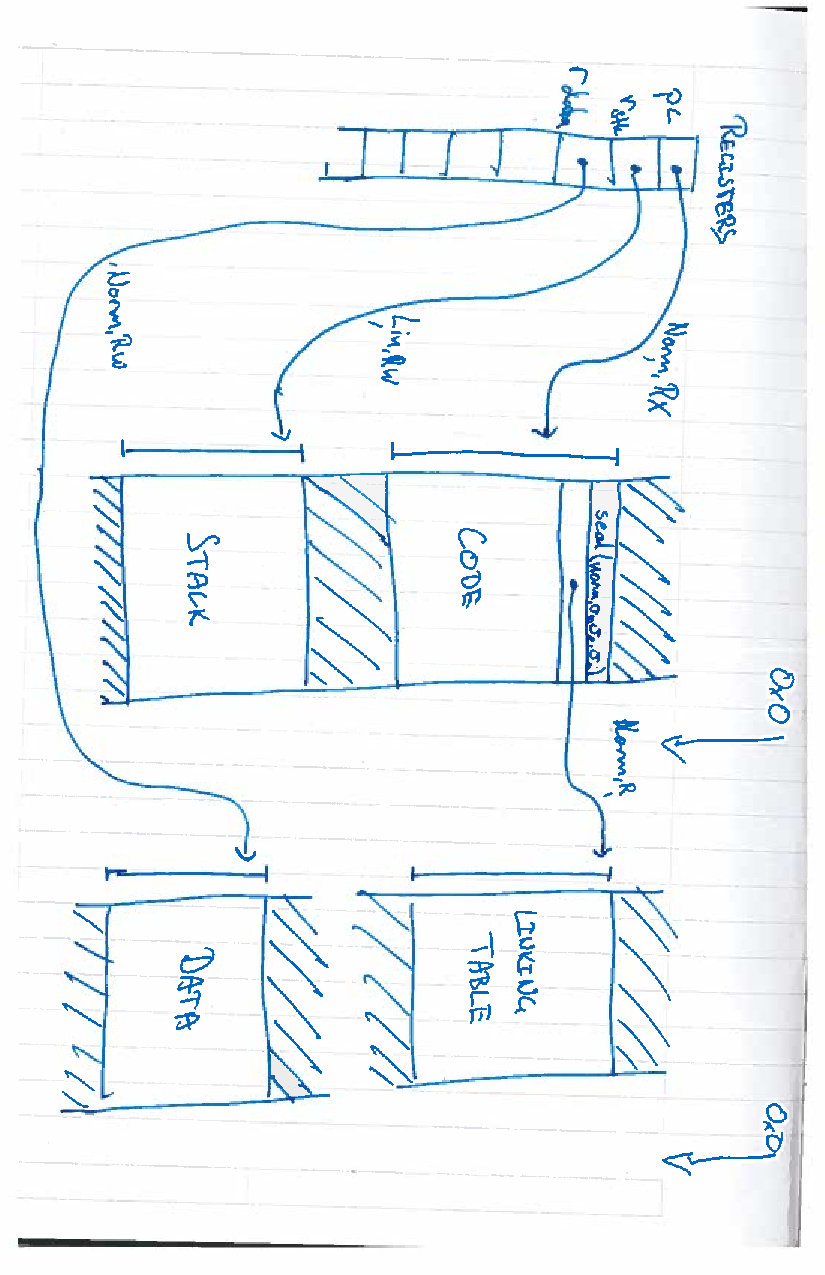
\includegraphics[angle=90,width=\textwidth]{img/linking.pdf}
  \caption{Linking and program layout (modulo the fact that the code memory contains a reference to the linking table, which is now no longer allowed).}
  \label{fig:trg-prog-link}
\end{figure}

\subsection{Components}
\label{sec:components}

A component can be either a component with a main (i.e. a program that still needs to be linked with library implementations) or one without (i.e. a library implementation that will be used by other components). 
It contains code memory, data memory a list of imported symbols, a list of exported symbols, a list of seals used for producing return capability pairs and a list of seals used for producing closures.

We define a component as follows:
\begin{align*}
  \var{comp}_0 &\mathrel{::=} (\mscode,\msdata,\overline{c_{\mathrm{import}}},\overline{c_{\mathrm{export}}},\sigrets,\sigcloss,A_\linear)\\
  \var{comp} &\mathrel{::=} \var{comp}_0\\
               &\mid  (\var{comp}_0,c_{\mathrm{main},c}, c_{\mathrm{main},d})
\end{align*}

We define inductively when a component is valid ($\vdash \var{comp}$) by the below inference rules:
\begin{mathpar}
  \inference{
    \mscode(a) = \seal{\sigma_\baddr,\sigma_\eaddr,\sigma_\baddr} & [\sigma_\baddr,\sigma_\eaddr] \subseteq (\sigrets \cup \sigcloss)
  }{
    \sigrets,\sigrets[\mathrm{owned}],\sigcloss \vdash_{\mathrm{comp-code}} \mscode,a
  }
  \and
  \inference{
    \mscode(a) \in \ints\\
    \mscode([a \cdots a + \calllen-1]) = \scall[0..\calllen-1]{\offpc,\offsigma}{r_1}{r_2} \Rightarrow (\mscode(a+\offpc) = \seal{\sigma_\baddr,\sigma_\eaddr,\sigma_\baddr} \wedge \sigma_\baddr+\offsigma \in \sigrets[\mathrm{owned}])
  }{
    \sigrets,\sigrets[\mathrm{owned}],\sigcloss \vdash_{\mathrm{comp-code}} \mscode,a
  }
  \and
  \inference{
    \exists d_\sigma : \dom(\mscode) \rightarrow \powerset{\Seal} \ldotp
    \sigrets = \biguplus_{a \in \dom(\mscode)} d_\sigma(a) \tand\\
    \forall a \in \dom(\mscode) \ldotp 
    \sigrets,d_\sigma(a),\sigcloss \vdash_{\mathrm{comp-code}} \mscode,a
  }{
    \sigrets,\sigcloss \vdash_{\mathrm{comp-code}} \mscode
  }
\end{mathpar}

\begin{mathpar}
  \inference{
  }{
    A_{\mathrm{code}},A_{\mathrm{own}},A_{\mathrm{non-linear}},\overline{c_{\mathrm{import}}},\sigrets,\sigcloss \vdash_{\mathrm{comp-value}} z
  }
  \and
  \inference{
    c \in \overline{c_{\mathrm{import}}}
  }{
    A_{\mathrm{code}},A_{\mathrm{own}},A_{\mathrm{non-linear}},\overline{c_{\mathrm{import}}},\sigrets,\sigcloss \vdash_{\mathrm{comp-value}} c
  }
  \and
  \inference{
    [\baddr,\eaddr] \subseteq A_{\mathrm{code}} & 
    \sigma \in \sigcloss
  }{
    A_{\mathrm{code}},A_{\mathrm{own}},A_{\mathrm{non-linear}},\overline{c_{\mathrm{import}}},\sigrets,\sigcloss \vdash_{\mathrm{comp-value}} \sealed{\sigma,((\rx,\normal),\baddr,\eaddr,\aaddr)}
  }
  \and
  \inference{
    \permbnf \sqsubseteq \rw&
    \lin = \linear \Rightarrow \emptyset \subset [\baddr,\eaddr] \subseteq A_{\mathrm{own}} &
    \lin = \normal \Rightarrow [\baddr,\eaddr] \subseteq A_{\mathrm{non-linear}}
  }{
    A_{\mathrm{code}},A_{\mathrm{own}},A_{\mathrm{non-linear}},\overline{c_{\mathrm{import}}},\sigrets,\sigcloss \vdash_{\mathrm{comp-value}} ((\perm,\lin),\baddr,\eaddr,\aaddr)
  }
  \and
  \inference{
    A_{\mathrm{code}},A_{\mathrm{own}},A_{\mathrm{non-linear}},\overline{c_{\mathrm{import}}},\sigrets,\sigcloss \vdash_{\mathrm{comp-value}} \vsc \\
    \sigma \in \sigcloss
  }{
    A_{\mathrm{code}},A_{\mathrm{own}},A_{\mathrm{non-linear}},\overline{c_{\mathrm{import}}},\sigrets,\sigcloss \vdash_{\mathrm{comp-value}} \sealed{\sigma,\vsc}
  }
\end{mathpar}

\begin{mathpar}
  \inference{
    \dom(\mscode) \mathrel{\#} \dom(\msdata)\\
    \sigrets,\sigcloss \vdash_{\mathrm{comp-code}} \mscode \\
    \exists A_\mathrm{own} : \dom(\msdata) \rightarrow \powerset{\dom(\msdata)} & \dom(\msdata) = A_{\mathrm{non-linear}} \uplus A_\linear \\
    A_\linear = \biguplus_{a \in \dom(\msdata)} A_{\mathrm{own}}(a) \\
    \forall a \in \dom(\msdata)\ldotp \dom(\mscode),A_{\mathrm{own}}(a),A_{\mathrm{non-linear}},\overline{c_{\mathrm{import}}},\sigrets,\sigcloss \vdash_{\mathrm{comp-value}} \msdata(a)\\
    \overline{\dom(\mscode), \emptyset, A_{\mathrm{non-linear}}, \overline{c_{\mathrm{import}}}, \sigrets,\sigcloss \vdash_{\mathrm{comp-value}} c_{\mathrm{export}}}\\
    \overline{c_{\mathrm{export}}} \mathrel{\#} \overline{c_{\mathrm{import}}} & (\dom(\mscode) \subseteq \ta) \vee (\dom(\mscode) \mathrel{\#} \ta)
  }{
    \vdash (\mscode,\msdata,\overline{c_{\mathrm{import}}},\overline{c_{\mathrm{export}}},\sigrets,\sigcloss,A_\linear)
  }
  \and
  \inference{
    \var{comp}_0 = (\mscode,\msdata,\overline{c_{\mathrm{import}}},\overline{c_{\mathrm{export}}},\sigrets,\sigcloss,A_\linear)\\
    \vdash \var{comp}_0 & c_{\mathrm{main},c}, c_{\mathrm{main},d} \in \overline{c_{\mathrm{export}}}
  }{
    \vdash (\var{comp}_0,c_{\mathrm{main},c}, c_{\mathrm{main},d})
  }
\end{mathpar}

\subsection{Linking}
\label{sec:linking}

\begin{mathpar}
  \inference{
    \var{comp}_1 = (\mscode[1], \msdata[1], \overline{c_{\mathrm{import},1}}, \overline{c_{\mathrm{export},1}}, \sigrets[1], \sigcloss[1],A_{\linear,1})\\
    \var{comp}_2 = (\mscode[2], \msdata[2], \overline{c_{\mathrm{import},2}}, \overline{c_{\mathrm{export},2}}, \sigrets[2], \sigcloss[2],A_{\linear,2})\\
    \var{comp}_3 = (\mscode[3], \msdata[3], \overline{c_{\mathrm{import},3}}, \overline{c_{\mathrm{export},3}}, \sigrets[3], \sigcloss[3],A_{\linear,3})\\
    \mscode[3] = \mscode[1] \uplus \mscode[2] &
    \msdata[3] = \msdata[1] \uplus \msdata[2] \\
    \overline{c_{\mathrm{export},3}} = \overline{c_{\mathrm{export},1}} \cup \overline{c_{\mathrm{export},2}}&
    \overline{c_{\mathrm{import},3}} = (\overline{c_{\mathrm{import},1}} \cup \overline{c_{\mathrm{import},2}}) \setminus \overline{c_{\mathrm{export},3}}\\
    \sigrets[3] = \sigrets[1] \uplus \sigrets[2] &
    \sigcloss[3] = \sigcloss[1] \uplus \sigcloss[2] &
    A_{\linear,3} = A_{\linear,1} \uplus A_{\linear,2}\\
    \dom(\mscode[3]) \mathrel{\#} \dom(\msdata[3]) & \sigrets[3] \mathrel{\#} \sigcloss[3]
  } {
    \var{comp}_3 = \var{comp}_1 \bowtie \var{comp}_2
  }
  \and
  \inference{
    \var{comp}_0'' = \var{comp}_0 \bowtie \var{comp}_0'
  }{
    (\var{comp}_0'',c_{\mathrm{main},c}, c_{\mathrm{main},d}) = \var{comp}_0 \bowtie (\var{comp}_0',c_{\mathrm{main},c}, c_{\mathrm{main},d})
  }
  \and
  \inference{
    \var{comp}_0'' = \var{comp}_0 \bowtie \var{comp}_0'
  }{
    (\var{comp}_0'',c_{\mathrm{main},c}, c_{\mathrm{main},d}) = (\var{comp}_0,c_{\mathrm{main},c}, c_{\mathrm{main},d}) \bowtie \var{comp}_0'
  }
\end{mathpar}

% update: linking no longer preserves well-formedness because we require is entirely trusted or not trusted at all.
% \begin{lemma}[Linking preserves component well-formedness]
%   \label{lem:linking-well-formedness}
%   If $\vdash \var{comp}_1$ and $\vdash \var{comp}_2$, then $\vdash \var{comp}_1 \bowtie \var{comp}_2$.
% \end{lemma}
% \begin{proof}
%   Follows by induction on the component validity judgement and definition-chasing.
%   The most interesting point is related to imports that are resolved from the other component during linking, but we know that those exports satisfy the $\mathrm{comp-value}$ judgement.
% \end{proof}

\subsection{Programs, contexts, initial execution configuration}
\label{sec:programs}

A program is intuitively a component that is ready to be executed, i.e. it must have an empty import list and a pair of capabilities to be used as main.
A context for a given component is any other component that can be linked with it to produce a program.

\begin{definition}[Programs and Contexts]
  We define a program to be a component $(\var{comp}_0,c_{\mathrm{main},c}, c_{\mathrm{main},d})$ with an empty import list.

  A context for a component $\var{comp}$ is another component $\var{comp}'$ such that $\var{comp} \bowtie \var{comp}'$ is a program.
\end{definition}

\begin{definition}[Initial execution configuration]
  \begin{mathpar}
    \inference{
      \reg(\pcreg) = c_{\mathrm{main},c} & 
      \reg(\rdata) = c_{\mathrm{main},d} \\
      \src{\reg(\rstk) = \stkptr{\rx,\baddr_\stk,\eaddr_\stk,\eaddr_\stk}} & 
      \trg{\reg(\rstk) = ((\rx,\linear),\baddr_\stk,\eaddr_\stk,\eaddr_\stk)} \\
      \reg(\RegName \setminus \{\pcreg,\rdata,\rstk\}) = 0\\
      \range{\ms_\stk} = \{0\}&
      \mem = \mscode \uplus \msdata \trg{\;\uplus\; \ms_\stk} \\
      [\baddr_\stk,\eaddr_\stk] = \dom(\ms_\stk ) \mathrel{\#} (\dom(\mscode) \cup \dom(\msdata)) &
      \overline{c_{\mathrm{import}}} = \emptyset
    }{
      ((\mscode, \msdata, \overline{c_{\mathrm{import}}}, \overline{c_{\mathrm{export}}}, \sigrets, \sigcloss,A_\linear),  c_{\mathrm{main},c}, c_{\mathrm{main},d}) \rightsquigarrow (\mem, \reg\src{, \emptyset, \ms_\stk})
    }
  \end{mathpar}
\end{definition}

\begin{definition}[Plugging a program into a context]
  When $\var{comp'}$ is a context for component $\var{comp}$ and $\var{comp}' \bowtie \var{comp} \rightsquigarrow \Phi$, 
  then we write $\plug{\var{comp'}}{\var{comp}}$ for the execution configuration $\Phi$.
\end{definition}

\section{Compiler}
\label{sec:compiler}

The compiler is the identity.

\section{Logical Relation}
In the following definitions, \src{blue} is used to indicate values related to the source machine. This is unlike previous definitions, where \src{blue} was used to indicate source language specific parts of definitions.
\subsection{Worlds}
\[
  \World = \Worldh \times \Worlds \times \Worldfs
\]
with $\Worlds$, $\Worldh$, and $\Region$ defined as follows
\[
  \Worldh = \RegionName \parfun (\Regions + \Regionh)
\]
and
\[
  \Worlds = \RegionName \parfun (\Regions \times \Addr)
\]
and
\[
  \Worldfs = \RegionName \parfun \Regions
\]
where $\RegionName = \nats$.
\begin{multline*}
  \Regionh = 
  \{\pure \} \times (\World \monnefun \URel{\MemSeg^2}) \times \\
  (\Seal \parfun \World \monnefun \URel{\SealableCaps \times \SealableCaps})
\end{multline*}
and
\[
  \Regions = \left\{
  \begin{array}{l}
    \{\spatial \} \times (\World \monnefun \URel{\MemSeg^2}) \uplus \\
    \{\spatialo \} \times (\World \monnefun \URel{\MemSeg^2})\uplus \\ 
    \{\revoked\}
  \end{array} \right.
\]
where $\spatial$ and $\spatialo$ are regions governing segments of memory addressed by linear capabilities.
$\spatialo$ signifies that this region is addressable.
$\spatial$ signifies that the region is not owned and can thus not be addressed.
At the same time it signifies that if something else addresses it, it is a $\linear$ capability.
Finally, $\pure$ signifies that the region is only addressed by non-linear capabilities.
Notice that no region allows for both linear and non-linear capabilities to address it.
Notice also that $\pure$ regions have an additional component that allows them to claim ownership of part of the address space of seals and impose a relational invariant on everything signed with those seals.

\dominique{Remaining question: what exactly does $\nsubeq$ on a UPred mean?  Does it mean subset ``up to n (including)'' or ``up to n-1 (including)''?
  Check what we can require without breaking contractiveness of recursive definition of value relation and/or what we did in previous paper and/or what we need in FTLR proof.
  Update: in the FTLR proof, we seem to need ``up to n'' because the heap predicate of the standard region is contractive in terms of the value relation.
  This also means we can afford to use ``up to n'' without breaking contractiveness of the recursive definition of the value relation.
  }
We have the following notion of regions being an $n$-subset of another region.
\begin{mathpar}
  \inferrule{ \forall \hat{W} \ldotp H \; \hat{W} \nsubeq H' \; \hat{W}}
            { (v,H) \nsubeq (v',H') }
\and
  \inferrule{ \forall \hat{W} \ldotp H \; \hat{W} \nsubeq H' \; \hat{W}}
            { (\pure,H,H_\sigma) \nsubeq (v',H') }
\and
  \inferrule{ \forall \hat{W} \ldotp H \; \hat{W} \nsubeq H' \; \hat{W}}
            { (v,H) \nsubeq (\pure,H',H_\sigma) }
\and
  \inferrule{ \forall \hat{W} \ldotp H \; \hat{W} \nsubeq H' \; \hat{W}}
            { (\pure,H,H_\sigma) \nsubeq (\pure,H',H_\sigma') }
\end{mathpar}
We define $n$-equality of regions $\iota \nequal \iota'$ as the symmetric closure, i.e. $\iota \nequal \iota'$ iff $\iota \nsubeq \iota'$ and $\iota \nsupeq \iota'$.

% \[
%   \Rels = \{(\phi_\pub, \phi) \in \powerset{\State^2}\times \powerset{\State^2} \mid \phi_\pub, \phi \text{ is reflexive and transitive and } \phi_\pub \subseteq \phi \}
% \]

We introduce a bit of notation for projecting out each part of the world:
\[
  \begin{array}{l}
    \pwheap = \pi_1(W)\\
    \pwpriv = \pi_2(W)\\
    \pwfree = \pi_3(W)
  \end{array}
\]
as well as projections for the regions:
\[
  \begin{array}{l}
  \prv{(v,s,\phi_\pub,\phi,H)} = v \\
  \prv{\revoked} = \revoked     
  \end{array}
\]

We define erasure for worlds as follows:
\[
\erase{(W_{\mathrm{heap}},W_{\mathrm{priv}},W_{\mathrm{free}})}{S} =
  \left( \erase{W_{\mathrm{heap}}}{S},\erase{W_{\mathrm{priv}}}{S},\erase{W_{\mathrm{free}}}{S} \right)
\]
where erasure for each part of a world is defined as follows:
\[
\erase{W_{\mathrm{heap}}}{S} = \lambda r \ldotp \left\{
    \begin{array}{l}
      \prv{W_{\mathrm{heap}}(r)} \in S\\
      \bot
    \end{array}
  \right.
\]
\[
\erase{W_{\mathrm{priv}}}{S} = \lambda r \ldotp \left\{
    \begin{array}{l}
      \prv{\pregion{W_{\mathrm{priv}}(r)}} \in S \\
      \bot
    \end{array}
  \right.
\]
\[
\erase{W_{\mathrm{free}}}{S} = \lambda r \ldotp \left\{
    \begin{array}{l}
      \prv{W_{\mathrm{free}}(r)} \in S\\
      \bot
    \end{array}
  \right.
\]

The $\activeReg{}$ function takes a world and filters away all the revoked regions, so
\[
  \activeReg{W} = \erase{W}{\spatial,\spatialo,\pure}
\]

Disjoint union of worlds. Joins together two alike worlds with strictly disjoint ownership over $\spatialo$-regions. Two worlds can be joined together if all of their three parts agree on the region names and each of their regions can be joined together.
\[
  W_1 \oplus W_2 = W
  \text{ iff }
  \begin{array}[t]{l}
    \dom(\pwheap) = \dom(\pwheap[W_1]) = \dom(\pwheap[W_2]) \tand \\
    \dom(\pwfree) = \dom(\pwfree[W_1]) = \dom(\pwfree[W_2]) \tand \\
    \dom(\pwpriv) = \dom(\pwpriv[W_1]) = \dom(\pwpriv[W_2]) \tand \\
    \forall r \in \dom(\pwheap) \ldotp \pwheap(r) = \pwheap[W_1](r) \oplus \pwheap[W_2](r) \tand \\
    \forall r \in \dom(\pwfree) \ldotp \pwfree(r) = \pwfree[W_1](r) \oplus \pwfree[W_2](r) \tand \\
    \forall r \in \dom(\pwpriv) \ldotp \pi_1(\pwpriv(r)) = \pi_1(\pwpriv[W_1](r)) \oplus \pi_1(\pwpriv[W_2](r))
  \end{array}
\]
$\oplus$ on regions is defined as follows
\begin{align*}
  (\pure,H,H_\sigma) \oplus (\pure,H,H_\sigma) =  & \; (\pure,H,H_\sigma) \\
  (\spatial,H) \oplus (\spatial,H) =  & \; (\spatial,H) \\
  (\spatialo,H) \oplus (\spatial,H) = & \; (\spatial,H) \oplus (\spatialo,H)\\
                                           =  & \; (\spatialo,H)
\end{align*}
and for all other cases $\oplus$ is undefined. Specifically, $\oplus$ is not defined when both sides are a $\spatialo$-region. It is further not defined if the two sides do not agree on region type or heap or sealed value relations.

\begin{lemma}
  \label{lem:oplus-assoc-comm}
  $\oplus$ is associative and commutative.
\end{lemma}
\begin{proof}
  Follows easily from the definitions.
\end{proof}

We also define a second disjoint union operator of worlds:
\[
  W_1 \uplus W_2 = W
  \text{ iff }
  \begin{array}[t]{l}
    \dom(\pwheap) = \dom(\pwheap[W_1]) \uplus \dom(\pwheap[W_2]) \tand \\
    \dom(\pwfree) = \dom(\pwfree[W_1]) \uplus \dom(\pwfree[W_2]) \tand \\
    \dom(\pwpriv) = \dom(\pwpriv[W_1]) \uplus \dom(\pwpriv[W_2]) \\
  \end{array}
\]
The two operators $\uplus$ and $\oplus$ are quite different.
The difference is most clear in the treatment of pure regions: $\uplus$ allows both worlds to have the same pure region, while $\oplus$ forbids this.
To understand this different treatment ($W_1 \uplus W_2$ and $W_1 \oplus W_2$), you should understand that the two are intended for different usages of worlds.
The $W_1 \oplus W_2$ operator treats the worlds as specifications of authority: taking the disjoint union of worlds specifying non-exclusive ownership of a block of memory is allowed and produces a new world that also specifies non-exclusive ownership of world. 
The $W_1 \uplus W_2$  operator treats worlds as specifications of memory contents: taking the disjoint union of worlds specifying the presence of the same memory range is not allowed.
The latter operator is used in the logical relation for components which specifies (among other things) that the world should specify the presence of the component's data memory.
Linking two components then produces a new component with both components' data memory.
The linked component is then valid in a world that has the combined memory presence specifications, not the combined authority.
In other words, $\oplus$ specifies disjoint authority distribution, while $\uplus$ specifies disjoint memory allocation.

Note also that this picture is further complicated by our usage of non-authority-carrying $\spatial$ regions.
They are really only there in a world $W$ as a shadow copy of a $\spatialo$ region in another world $W'$ that $W$ will be combined with.
The shadow copy is used for specifying when a memory satisfies a world: the memory should contain all memory ranges that anyone has authority over, not just the ones whose authority belongs to the memory itself.
For example, if a register contains a linear pointer to a range of memory, then the register file will be valid in a world where the corresponding region is $\spatialo$, while the memory will be valid in a world with the corresponding region only $\spatial$.
However, for the memory to satisfy the world, the block of memory needs to be there, i.e. the memory should contain blocks of memory satisfying every region that is $\spatialo$, $\pure$, but also just $\spatial$ (because it may be $\spatialo$ in, for example, the register file's world).

\begin{lemma}
  \label{lem:uplus-assoc-comm}
  $\uplus$ is associative and commutative.
\end{lemma}
\begin{proof}
  Follows easily from the definitions.
\end{proof}

\begin{lemma}[Odd distributivity of $\oplus$ and $\uplus$]
  \label{lem:oplus-distr-uplus}
  \begin{equation*}
    (W_1\oplus W_2) \uplus (W_3 \oplus W_4) = (W_1 \uplus W_3) \oplus (W_2 \uplus W_4)
  \end{equation*}
  Also, the left expression is defined iff the right expression is.
\end{lemma}
\begin{proof}
  Follows by definition-chasing.
\end{proof}

\subsection{Future world}
% {\color{DarkGreen}
The future world relation becomes:
\begin{mathpar}
  \inferrule{ \text{for $i \in \{\mathrm{heap},\mathrm{free},\mathrm{priv} \}$} \\ \exists m_i : \RegionName \fun \RegionName, \text{ injective}\ldotp \dom(W'.i) \supseteq \dom(m_i(W.i)) \wedge \forall r \in \dom(W.i)\ldotp W'.i(m_i(r)) \future W.i(r) }
            { W' \future W }
\end{mathpar}
% The private future world relation becomes:
% \begin{mathpar}
%   \inferrule{ \text{for $i \in \{\mathrm{heap},\mathrm{free},\mathrm{priv} \}$} \\ \exists m_i : \RegionName \fun \RegionName, \text{ injective}\ldotp \dom(W'.i) \supseteq \dom(m_i(W.i)) \wedge \forall r \in \dom(W.i)\ldotp W'.i(m_i(r)) \privft W.i(r) \\  \exists r \in \dom(W'.\mathrm{priv}) \setminus \dom(m_{\mathrm{priv}}(\pwpriv))\ldotp \pwpriv[W'](r) \text{ is non-empty}}
%             { W' \future W }
% \end{mathpar}
% where we take ``is non-empty'' to mean the following:

% \begin{definition}
%   We say a region $(k,s,\phi_\pub,\phi,H)$ is non-empty iff
% \[
%   \begin{array}{l}
%     \forall n, \hat{W}\ldotp \forall \npair{\stpair{\ms}{\ms}} \in H \;  \hat{W} \ldotp \dom(\src{\ms_S}) > 0 \wedge \dom(\ms_T) > 0 
%   \end{array}
% \]
% \end{definition}

% }


% For both $\privft$ and $\pubft$ we have
% \begin{mathpar}
%   \inferrule{ \exists m : \RegionName \fun \RegionName, \text{ injective}\ldotp \dom(W') \supseteq \dom(m(W)) \wedge \forall r \in \dom(W)\ldotp W'(m(r)) \future W(r) }
%             { W' \future W }
% \end{mathpar}
%
Future regions allow $\spatial$ regions to become $\revoked$.
Also: the future region relation allows $\spatial$ regions to become $\spatialo$, which expresses that our system is affine, rather than linear.
\lau{22-3-2018: TODO need extra rules for regions with seal interpretations}
\begin{mathpar}
  \inferrule{ }{ \revoked \future (\spatial,\_)}
\and
  \inferrule{ }{ \revoked \future \revoked }
  \and
  \inferrule{ }{(\spatialo,H) \future (\spatial,H)}
  \and
  \inferrule{ }{(\spatialo,H) \future (\spatialo,H)}
  \and
  \inferrule{ }{(\spatial,H) \future (\spatial,H)}
% \and
%   \inferrule{ (s,s') \in \phi}
%             { (\spatialo,s',\phi_\pub,\phi,H) \privft (\spatial,s,\phi_\pub,\phi,H)  }
%             \and
%   \inferrule{ (s,s') \in \phi }
%             { (v,s',\phi_\pub,\phi,H) \privft (v,s,\phi_\pub,\phi,H)  }
\end{mathpar}
%
% Public future regions are allowed to transition according to the public part of their transition system.
% \begin{mathpar}
%     \inferrule{ }
%             { \revoked \pubft \revoked }
%             \and
%             \inferrule{}{(\spatialo,H) \privft (\spatial,H)}
%   %           \and
%   % \inferrule{ (s,s') \in \phi_\pub}
%   %           { (\spatialo,s',\phi_\pub,\phi,H) \pubft (\spatial,s,\phi_\pub,\phi,H)  }
%   %           \and
%   % \inferrule{ (s,s') \in \phi_\pub}
%   %           { (v,s',\phi_\pub,\phi,H) \pubft (v,s,\phi_\pub,\phi,H)  }
% \end{mathpar}

\begin{definition}[The pure part of a world]
  \label{def:purePart}
  For any world $W$, we define
  \begin{align*}
    \purePart{W} &\defeq (\purePart{\pwheap},\purePart{\pwpriv},\purePart{\pwfree})\\
    \purePart{W_\var{heap}} &\defeq
                       \begin{cases}
                         W_{\var{heap}}(r) & \text{if } W_\var{heap}(r) = (pure,\var{sm})\\
                         (\spatial,\var{sm}) & \text{if } W_\var{heap}(r) = (\spatial,\var{sm})\\
                         (\spatial,\var{sm}) & \text{if } W_\var{heap}(r) = (\spatialo,\var{sm})\\
                         \revoked & \text{if } W_\var{heap}(r) = \revoked\\
                       \end{cases}\\
    \purePart{W_\var{priv}} &\defeq
                       \begin{cases}
                         ((\spatial,\var{sm}),\opc) & \text{if } W_\var{priv}(r) = ((\spatial,\var{sm}),\opc)\\
                         ((\spatial,\var{sm}),\opc) & \text{if } W_\var{priv}(r) = ((\spatialo,\var{sm}),\opc)\\
                         (\revoked,\opc) & \text{if } W_\var{priv}(r) = (\revoked,\opc)\\
                       \end{cases}\\
    \purePart{W_\var{free}} &\defeq
                       \begin{cases}
                         W_{\var{free}}(r) & \text{if } W_{\var{free}}(r) = (pure,\var{sm})\\
                         (\spatial,\var{sm}) & \text{if } W_{\var{free}}(r) = (\spatial,\var{sm})\\
                         (\spatial,\var{sm}) & \text{if } W_{\var{free}}(r) = (\spatialo,\var{sm})\\
                         \revoked & \text{if } W_{\var{free}}(r) = \revoked\\
                       \end{cases}
  \end{align*}
\end{definition}

\begin{lemma}[purePart is duplicable]
  \label{lem:purePart-duplicable}
 For all $W$, we have that $W = W \oplus \purePart{W}$.
\end{lemma}
\begin{proof}
  Follows from the definition of $\purePart{}$ and $\oplus$.
\end{proof}

\begin{lemma}[purePart is idempotent]
  \label{lem:purePart-idempotent}
  For all $W$, we have that $\purePart{W} = \purePart{}(\purePart{W})$ and $\purePart{W} = \purePart{W} \oplus \purePart{W}$.
\end{lemma}
\begin{proof}
  The first part follows easily from the definition.
  The second statement follows from the first, together with Lemma~\ref{lem:purePart-duplicable}.
\end{proof}

\begin{lemma}[purePart is monotone]
  \label{lem:purePart-mono}
 For all $W'\future W$, we have that $\purePart{W'} \future \purePart{W}$.
\end{lemma}
\begin{proof}
  Follows easily from the definition of $\purePart{}$ and $\future$.
\end{proof}

\begin{lemma}[Increasing authority is the future]
  \label{lem:oplus-future}
  For all $W$, we have that:
  $W_1 \oplus W_2 \future W_1$
\end{lemma}
\begin{proof}
  Follows easily from the definitions.
\end{proof}

\begin{lemma}[Adding additional memory is the future]
  \label{lem:uplus-future}
  For all $W_1,W_2$, we have that:
  $W_1 \uplus W_2 \future W_1$
\end{lemma}
\begin{proof}
  Follows easily from the definitions.
\end{proof}



\begin{lemma}[Purity is a thing of the past]
  \label{lem:world-fut-purePart}
  For all $W$, we have that $W \future \purePart{W}$.
\end{lemma}
\begin{proof}
  Consequence of Lemmas~\ref{lem:purePart-duplicable}
  and~\ref{lem:oplus-future}.
\end{proof}

\subsection{Memory satisfaction}
\lau{14-02-2018: No matter what the memory satisfaction ends up looking like, remember to handle the revoked case.}
% {\color{DarkGreen}
\lau{RESOLVED add frame to memory satisfaction and remove it from observation relation.}
Memory satisfaction for new worlds:
\[
  \memSat{\ms_S,\ms_\stk,\stk,\ms_T}{W} \text{ iff } 
  \left\{
    \begin{array}{l}
      \stk = (\opc_0,\ms_0):: \dots :: (\opc_m,\ms_m) \wedge \\
      \ms_S \uplus \ms_\stk \uplus \ms_0 \uplus \dots \uplus \ms_m  \text{ is defined} \wedge\\
      W = W_{\var{stack}} \oplus W_{\var{free\_stack}} \oplus W_{\var{heap}} \wedge\\
      \exists \ms_\var{T,stack}, \ms_\var{T,free\_stack}, \ms_\var{T,heap}, \ms_{T,f}, \ms_{S,f}, \ms_S',\ldotp \\
      \quad \ms_S = \ms_{f,S} \uplus \ms_S' \wedge \\
      \quad \ms_T = \ms_\var{T,stack} \uplus \ms_\var{T,free\_stack} \uplus \ms_\var{T,heap} \uplus \ms_{T,f} \wedge \\

      \quad \memSatStack{\stk,\ms_\var{T,stack}}{W_{\var{stack}}} \wedge \\
      \quad \memSatFStack{\ms_\stk,\ms_\var{T,free\_stack}}{W_{\var{free\_stack}}} \wedge \\
      \quad \memSatHeap{\ms_S',\ms_\var{T,heap}}{W_{\var{heap}}}
    \end{array}
  \right.
\]

\[
  \memSatStack{\stk,\ms_T}{W} \text{ iff } 
  \left\{
    \begin{array}{l}
      W_\var{stack} = \pwpriv \wedge \\
      \stk = (\opc_0,\ms_0), \dots (\opc_m,\ms_m) \wedge \\
      \forall i \in \{0,\dots,m\} \ldotp (\dom(\ms_i) \neq \emptyset \wedge\\
      \quad \forall i < j \ldotp \forall a \in \dom(\ms_i) \ldotp \forall a' \in \dom(\ms_j) \ldotp a < a') \wedge\\
      \exists R_\ms : \dom(\activeReg{W_\var{stack}}) \fun \MemSeg \times \SealableCaps \times \MemSeg \ldotp \\
      \quad \ms_T = \biguplus_{r \in \dom(\activeReg{W_\var{stack}})} \pi_3(R_\ms(r)) \wedge \\
      \quad \ms_0 \uplus \dots \uplus \ms_m = \biguplus_{r \in \dom(\activeReg{W_\var{stack}})} \pi_1(R_\ms(r)) \wedge \\
      \quad \exists R_W : \dom(\activeReg{W_\var{stack}}) \fun \World \ldotp \\
      \qquad W = \bigoplus_{r \in \dom(\activeReg{W_\var{stack}})} R_W(r) \wedge \\
      \qquad \forall r \in \dom(\activeReg{W_\var{stack}})\ldotp \\
      \qquad \quad \npair{(\pi_1(R_\ms(r)),\pi_3(R_\ms(r))} \in W_\var{stack}(r).H \; \xi^{-1}(R_W(r)) \wedge\\
      \qquad \quad \pi_2(R_\ms(r)) = W_\var{stack}(r).\opc \wedge\\
      \qquad \quad \exists i \ldotp \opc_i = W_\var{stack}(r).\opc \wedge \ms_i = \pi_1 (R_\ms(r))
    \end{array}
  \right.
\]

\[
  \memSatFStack{ms_\stk,\ms_T}{W} \text{ iff } 
  \left\{
    \begin{array}{l}
      W_\var{stack} = \pwfree \wedge \\
      \exists R_\ms : \dom(\activeReg{W_\var{stack}}) \fun \MemSeg \times \MemSeg \wedge \\
      \quad \ms_T = \biguplus_{r \in \dom(\activeReg{W_\var{stack}})} \pi_2(R_\ms(r)) \wedge \\
      \quad \ms_\stk = \biguplus_{r \in \dom(\activeReg{W_\var{stack}})} \pi_1(R_\ms(r)) \wedge \\
      \quad \stkb \in \dom(\ms_T) \wedge \stkb \in \dom(\ms_\stk) \wedge \\
      \quad \exists R_W : \dom(\activeReg{W_\var{stack}}) \fun \World\ldotp\\
      \qquad W = \oplus_{r \in \dom(\activeReg{W_\var{stack}})} R_W(r) \wedge\\
      \qquad \forall r \in \dom(\activeReg{W_\var{stack}}) \ldotp \\
      \qquad \quad \npair{R_\ms(r)} \in  W_\var{stack}(r).H \; \xi^{-1}(R_W(r))
    \end{array}
  \right.
\]

\[
  \memSatHeap{ms,\ms_T}{W} \text{ iff } 
  \left\{
    \begin{array}{l}
      \exists R_\ms : \dom(\activeReg{\pwheap}) \fun \MemSeg \times \MemSeg \wedge \\
      \quad \ms_T = \biguplus_{r \in \dom(\activeReg{\pwheap})} \pi_2(R_\ms(r)) \wedge \\
      \quad \ms = \biguplus_{r \in \dom(\activeReg{\pwheap})} \pi_1(R_\ms(r)) \wedge \\
      \quad \exists R_W : \dom(\activeReg{\pwheap}) \fun \World\ldotp\\
      \qquad W = \oplus_{r \in \dom(\activeReg{\pwheap})} R_W(r) \wedge\\
      \qquad \forall r \in \activeReg{\pwheap} \ldotp \\
      \qquad \quad \npair{R_\ms(r)} \in  \pwheap(r).H \; \xi^{-1}(R_W(r)) \wedge\\
      \exists R_\var{seal} : \dom(\activeReg{\pwheap}) \fun \powerset{\Seal} \wedge\\
      \quad \biguplus_{r \in \dom(\activeReg{\pwheap})} R_\var{seal}(r)) \text{ is defined } \wedge\\
      \quad \dom(\pwheap(r).H_\sigma) = R_\var{seal}(r)
    \end{array}
  \right.
\]
% }



% \[
%   \memSat{\ms_S,\ms_\stk,\stk,\ms_T}{W} \text{ iff } 
%   \left\{
%     \begin{array}{l}
%       \exists R_\ms : \dom(W) \fun \MemSeg^2 \ldotp \\
%       \quad \ms_T = \biguplus_{r \in \dom(W)} \pi_2(R_\ms(r)) \wedge \\
%       \quad \stk = (\_,\ms_{\stk,0}) :: \dots :: (\_,\ms_{\stk,m}) \wedge \\
%       \quad \ms_S \uplus \ms_\stk \uplus \ms_{\stk,0} \uplus \dots \uplus \ms_{\stk,m} = \biguplus_{r \in \dom(W)} \pi_1(R_\ms(r)) \wedge \\
%       \quad \exists R_w : \dom(W) \fun \World \ldotp\\
%       \qquad W = \bigoplus_{r \in \dom(W)} R_w(r) \wedge \\
%       \qquad \forall r \in \dom(W) , n' < n \ldotp \\
%       \quad \qquad \npair[n']{R_\ms(r)} \in W(r).H \; (\xi^{-1} (R_w (r))) 
%     \end{array}
%   \right.
% \]
% In the definition of memory satisfaction, $R_\ms$ creates a partitioning of the two related memories. As the source language is a special interpretation of the target language, part of the target memory needs to relate to the stack in the source language. We also need to split up the world which is done by $R_W$.We split up the world in order to make sure that the linearity constraints imposed by the world are satisfied.
% \lau{30-10-2017: It is not clear to me whether this definition should also talk about $\opc$.}
% \dominique{4-12-2017: Regarding the question whether $\opc$ should be mentioned in the memory satisfaction relation.
%   The relevant intuitive aspect of the proof here, I think, is that on a return, the source semantics restores opc from the copy kept in the stack, while the target semantics restores it from the copy in the code part of the return pointer.
%   We will need to prove (somewhere) that these two correspond, which means we will need to track of the invariant that guarantees this somewhere (perhaps here?).
%   I suspect the relevant invariants are (1) that any executable pointer signed with $\sealAss{a}$ must point to $a + \calllen$ and (2) that anything related to a $\rretc$ must be executable and sealed.
%   Perhaps this invariant is easiest to track in (1) the general requirement on the $H_\sigma$ and (2) in the value relation.
%   This suggests nothing should be required about opc here?
%   To be confirmed in the proof of the fundamental theorem.
% }

\begin{lemma}[Combined independent heap memory satisfies disjoint world]
  \label{sec:combined-memory-disjoint-world}
  If $\memSatHeap{\overline{\sigma_1},ms_{S,1},\ms_{T,1}}{W_1}$ and $\memSatHeap{\overline{\sigma_2},ms_{S,2},\ms_{T,2}}{W_2}$, then $\memSatHeap{\overline{\sigma_1}\uplus\overline{\sigma_2},ms_{S,1}\uplus \ms_{S,2},\ms_{T,1}\uplus \ms_{T,2}}{W_1 \uplus W_2}$.
\end{lemma}
\begin{proof}
  Unfolding the definitions, it's easy to construct the memory and seal partitions $R_{\ms,3}$ and $R_{\var{seal},3}$ from the corresponding partitions of the separate memories.
  Constructing $R_{W,3}$ from $R_{W,1}$ and $R_{w,2}$ is a bit harder, but we can use Lemmas~\ref{lem:oplus-distr-uplus},~\ref{lem:purePart-duplicable},~\ref{lem:uplus-assoc-comm} and~\ref{lem:oplus-assoc-comm} to manipulate the world equalities as follows:
  \begin{align*}
    W_1 \uplus W_2 &= (\purePart{W_1} \oplus W_1) \uplus (W_2 \oplus \purePart{W_2})\\
                   &= (\purePart{W_1} \uplus W_2) \oplus (W_1 \uplus \purePart{W_2})\\
                   &= (\purePart{W_1} \uplus \bigoplus_r R_{W,2}(r)) \oplus ((\bigoplus_r R_{W,1}(r)) \uplus \purePart{W_2})\\
                   &= \bigoplus_r (\purePart{W_1} \uplus R_{W,2}(r)) \oplus \bigoplus_r (R_{W,1}(r) \uplus \purePart{W_2})
  \end{align*}
  We can then define
  \begin{equation*}
    R_{W,3}(r) =
    \begin{cases}
      \purePart(W_1) \uplus R_{W,2}(r) &\text{when } r \in \dom(R_{W,2})\\
      \purePart(W_2) \uplus R_{W,1}(r) &\text{when } r \in \dom(R_{W,1})
    \end{cases}
  \end{equation*}
  Lemma~\ref{lem:uplus-future} and the monotonicity of the regions' memory predicates then yield the required results.
\end{proof}

\subsection{Relation}
% \lau{19-10-2017: Rest of source configuration needs to come from somewhere in $\lre$.}
% \[
%   \lre(W) = \left\{ \npair{\stpair[.]{v_{c,S},v_{d,S}}{v_{c,T},v_{d,T}}} \middle| 
%     \begin{array}{l}
%       \forall n' \leq n, \src{\reg_S}, \reg_T, \src{\ms_S}, \ms_T, \src{\ms_\stk}, \src{\stk} \ldotp\\
%       \quad \forall W_\lrr, W_\lrm \ldotp \\
%       \qquad\npair[n']{[\stpair[.]{v_{c,S}}{v_{c,T}},\stpair[.]{v_{d,T}}{v_{d,S}}]} \in \lrp(W) \wedge \\
%       \qquad\npair[n']{\stpair{\reg}{\reg}} \in \lrr(W_\lrr) \wedge\\
%       \qquad\memSat[n']{\stpair[.]{\ms_S,\stk,\ms_\stk}{\ms_T}}{W_\lrm} \wedge\\
%       \qquad W_{\var{new}} = W \oplus W_\lrr \oplus W_\lrm \\
%       \qquad\Rightarrow\\
%       \qquad\npair[n']{\left(\array{l}\src{(\ms_S,\reg_S\updReg{\pcreg,\rdata}{v_{c,S},v_{d,S}},\stk, \ms_\stk)},\\
%                                           (\ms_T,\reg_T\updReg{\pcreg,\rdata}{v_{c,T},v_{d,T}})
%                        \endarray\right)}
%       \in \lro
%     \end{array}
%     \right\}
% \]
% \lau{24-10-2017: Dominique, I do not see how the splitting of worlds is going to work out. I can see how it will enforce linearity, but if you give a "spatial" region (the kind of region that is only allowed to go to one part of a split) to the $\lrr$-relation, then the memory satisfaction does not have it, and it cannot find a memory segment for this part. In other words, the memory satisfaction will not be able to find a concrete memory segment for segments governed by a linear capability in the register file. Maybe the memory satisfaction should have all of the parts, so it can represent them (but also limit what linear capabilities can be used).}
% \dominique{18-1-2018: Lau, I suppose the above has been answered verbally already during one of the previous skype calls, but for reference, this is what the spatial vs spatial\_owned distinction is intended to solve: the world will contain spatial regions for such memory segments, but not spatial\_owned ones, so the memory satisfaction will require the memory to be present but not allow it to be addressed.}

% \dominique{22-1-2018: the below is an alternative proposal to the above definition. It is part of a proposed refactoring to simplify the merge the cases for return pointers and closures in the value relation.}
Two expression relations: one for sealed code-data pairs being jumped to and one for capabilities being jumped to in the regular way.
The argument for having one relation relate pairs of pairs of capabilities and the other relate pairs of capabilities is that that is how xjump and regular jumps work: xjump takes pairs while regular jumps take single capabilities.
\begin{align*}
  \lrexjg{\trust}(W) &= \left\{ \npair{\stpair[.]{v_{c,S},v_{d,S}}{v_{c,T},v_{d,T}}} \middle| 
    \begin{array}{l}
      \forall n' \leq n, \src{\reg_S}, \reg_T, \src{\ms_S}, \ms_T, \src{\ms_\stk}, \src{\stk} \ldotp\\
      \quad \forall W_\lrrs , W_\lrm \ldotp \\
      \qquad\npair[n']{\stpair{\reg}{\reg}} \in \lrrg{\trust}(\{\rdata\}) (W_\lrrs ) \wedge\\
      \qquad\memSat[n']{\stpair[.]{\ms_S,\stk,\ms_\stk}{\ms_T}}{W_\lrm} \wedge \\
      \qquad\Phi_S = \src{(\ms_S,\reg_S,\stk, \ms_\stk)}\wedge\\
      \qquad\Phi_T = (\ms_T,\reg_T) \wedge\\
      \qquad W \oplus W_\lrrs \oplus W_\lrm \text{ is defined }\\
      \qquad\Rightarrow \exists \Phi_S',\Phi_T'\ldotp\\
      \quad\qquad \Phi_S' = \xjumpResult{v_{c,S}}{v_{d,S}}{\Phi_S} \tand\\
      \quad\qquad\Phi_T' = \xjumpResult{v_{c,T}}{v_{d,T}}{\Phi_T}\tand\\
      \quad\qquad\npair[n']{\left(\Phi_S', \Phi_T' \right)}\in \lro
    \end{array}
    \right\}\\
  \lreg{\trust}(W) &= \left\{ \npair{\stpair[.]{v_{c,S}}{v_{c,T}}} \middle| 
    \begin{array}{l}
      \forall n' \leq n, \src{\reg_S}, \reg_T, \src{\ms_S}, \ms_T, \src{\ms_\stk}, \src{\stk} \ldotp\\
      \quad \forall W_\lrrs , W_\lrm \ldotp \\
      \qquad\npair[n']{\stpair{\reg}{\reg}} \in \lrrg{\trust} (W_\lrrs ) \wedge\\
      \qquad\memSat[n']{\stpair[.]{\ms_S,\stk,\ms_\stk}{\ms_T}}{W_\lrm} \\
      \qquad\Phi_S = \src{(\ms_S,\reg_S,\stk, \ms_\stk)}\\
      \qquad \Phi_S' = \Phi_S \updReg{\pcreg}{v_{c,S}}\\
      \qquad\Phi_T = (\ms_T,\reg_T)\\
      \qquad\Phi_T' = \Phi_T\updReg{\pcreg}{v_{c,T}}\\
      \qquad W \oplus W_\lrrs \oplus W_\lrm\\
      \qquad\Rightarrow\npair[n']{\left(\Phi_S', \Phi_T' \right)}\in \lro
    \end{array}
    \right\}
\end{align*}
 
\[
  \lrol = \left\{ \npair{\left(\array{l}\src{(\ms_S,\reg_S,\stk_S,\ms_{\stk,S})},\\(\ms_T,\reg_T)\endarray\right)} \middle|
    \begin{array}{l}
      \forall i \leq n \ldotp \\
      \quad \src{(\ms_S,\reg_S,\stk_S,\ms_{\stk,S})} \sterm[i]{\ta,\stkb} \Rightarrow (\ms_T,\reg_T) \term\\
    \end{array}
\right\}
\]
\[
  \lror = \left\{ \npair{\left(\array{l}\src{(\ms_S,\reg_S,\stk_S,\ms_{\stk,S})},\\(\ms_T,\reg_T)\endarray\right)} \middle|
    \begin{array}{l}
      \forall i \leq n \ldotp \\ 
      \quad (\ms_T ,\reg_T) \term[i] \Rightarrow \src{(\ms_S,\reg_S,\stk_S,\ms_{\stk,S})} \sterm{\ta,\stkb}
    \end{array}
\right\}
\]


\lau{RESOLVED make this only take a pair (the other uses are gone)}
\[
  \lrp(W) = \left\{ \npair{(\lin,\baddr,\eaddr)} \middle|
    \begin{array}{l}
      \exists r \in \addressable{l,W} \ldotp\\
      \quad \forall \npair{\stpair{\ms}{\ms}} \in S(i)(r).H \; \xi^{-1}(W)  \ldotp \\
      \qquad \dom(\src{\ms_S}) \supseteq [\baddr,\eaddr] \wedge \dom(\ms_T) \supseteq [\baddr,\eaddr]
    \end{array}
  \right\}
\]


\[
  \lrrg{\trust}(R)(W) = \left\{ \npair{\stpair{\reg}{\reg}} \middle|
    \begin{array}{l}
      \exists S : (\RegName \setminus (\{\pcreg \} \cup R))\fun \World \ldotp \\
      \quad W = \bigoplus_{r \in (\RegName\setminus (\{\pcreg,\rdata \} \cup R))} S(r) \wedge \\
      \quad \forall r \in \RegName \setminus (\{\pcreg \} \cup R)\ldotp\\
      \qquad\npair{\stpair[.]{\src{\reg_S(r)}}{\reg_T(r)}} \in \lrvg{\trust}(S(r))
    \end{array}
            \right\}
\]
We write $\lrr(W)$ to mean $\lrr(\emptyset)(W)$. That is, if we do not need to exclude extra registers, then we simply omit that argument.
% DOMI 18-1-2018: the below remark is obsolete, so I commented it out.
% Where $S\text{ is a separation of $W$}$ means that no two partition share the same ``spatial'' region (whatever that is).
%\dominique{18-1-2018: it might be convenient to exclude $\rdata$ from the $\lrr$ relation by default too. Check if we ever use it with other instantiations of R.}
% Lau 19-01-2018: Added rdata as default.
\lau{RESOLVED check what conditions need to have a ``square'' i.e. need approximation}
\[
  \lrv(W) =
  \begin{array}[t]{l}
    \left\{ \npair{\stpair[.]{i}{i}} \;\middle|\; i \in \ints \right\}\cup \\
%
    \left\{ \npair{\left(\arraycolsep=0pt\array{l}\src{\sealed{\sigma,\vsc_S}},\\ \sealed{\sigma,\vsc_T} \endarray\right)} \;\middle| \;
    \begin{array}{l}
      \exists r \in \dom(\pwheap)\ldotp \pwheap(r) = (\pure,\_,H_\sigma) \tand \\
      \quad \npair[n']{\stpair[.]{\vsc_S}{\vsc_T}} \in H_\sigma \; \sigma \; \xi^{-1}(W) \text{ for all $n' < n$}\wedge\\
      \quad (\isLinear{\src{\vsc_S}} \text{ iff } \isLinear{\vsc_T}) \wedge\\
      \quad (\isLinear{\src{\vsc_S}} \Rightarrow \\
      \qquad\forall W' \future W, W_o, n' < n, \npair[n']{\stpair[.]{\vsc_S'}{\vsc'_T}} \in H_\sigma \; \sigma \; \xi^{-1}(W_o) \ldotp \\
      \qquad \quad \npair[n']{\src{\vsc_S},\src{\vsc_S'},\vsc_T,\vsc_T'} \in \lrexj(W'\oplus W_o)) \wedge \\
      \quad (\nonLinear{\src{\vsc_S}} \Rightarrow \\
      \qquad \forall W' \future \purePart{W}, W_o, n' < n, \npair[n']{\stpair[.]{\vsc_S'}{\vsc'_T}} \in H_\sigma \; \sigma \; \xi^{-1}(W_o) \ldotp \\
      \qquad \quad \npair[n']{\src{\vsc_S},\src{\vsc_S'},\vsc_T,\vsc_T'} \in \lrexj(W'\oplus W_o))

      % This case was never used (?) so it is not necessary.
      % \wedge \\
      % \quad \npair[n']{\src{\vsc_S'},\src{\vsc_S},\vsc_T',\vsc_T} \in \lrexj(W' \oplus W_o)
    \end{array}
    \right\}\cup\\
    \left\{ \npair{\left(\arraycolsep=0pt\array{l} \src{\seal{\sigma,\sigma_\baddr,\sigma_\eaddr}},\\ \seal{\sigma,\sigma_\baddr,\sigma_\eaddr} \endarray \right)} 
    \; \middle| \;
    \begin{array}{l}
      \forall \sigma' \in [\sigma_\baddr,\sigma_\eaddr] \ldotp \exists r \in \dom(\pwheap) \ldotp \\
      \quad \pwheap(r) = (\pure,\_,H_\sigma) \tand H_\sigma \; \sigma' \nequal \lrv
    \end{array}
    \right\} \cup \\
    \left\{ \npair{\left(\arraycolsep=0pt\array{l} \src{\stkptr{\perm,\baddr,\eaddr,\aaddr}},\\ ((\perm,\linear),\baddr,\eaddr,\aaddr) \endarray \right)} \;\middle|\;
    \begin{array}{l}
      \begin{array}{r l l}
        \perm = \noperm & \Rightarrow & \npair{(\linear,\baddr,\eaddr)} \in \lrp(W) \wedge \\
        \perm \in \readAllowed{} &\Rightarrow& \npair{[\baddr,\eaddr]} \in \stackReadCond{W} \wedge \\
        \perm \in \writeAllowed{} &\Rightarrow& \npair{[\baddr,\eaddr]} \in \stackWriteCond{W}
      \end{array}
    \end{array}
    \right\} \cup \\
%
    \left\{ \npair{\left(\arraycolsep=0pt\array{l} \src{((\perm,\lin),\baddr,\eaddr,\aaddr)},\\ ((\perm,\lin),\baddr,\eaddr,\aaddr) \endarray \right)} \;\middle|\; 
    \begin{array}{l}
      \begin{array}{r l l }
        \perm = \noperm & \Rightarrow & \npair{(\lin,\baddr,\eaddr)} \in \lrp(W) \wedge \\
        \perm \in \readAllowed{} &\Rightarrow& \npair{[\baddr,\eaddr]} \in \readCond{\lin,W} \wedge\\
        \perm \in \writeAllowed{} &\Rightarrow& \npair{[\baddr,\eaddr]} \in \writeCond{\lin,W} \wedge\\
        % we are excluding rwx pointers.
        \perm \neq \rwx \wedge \\
        % \perm = \rwx &\Rightarrow& \array[t]{l}\npair{(\{\rwx,\rx\},\baddr,\eaddr)} \in \execCond{\lin,W} \wedge \\
        %                            \npair{(\baddr,\eaddr)} \in \xReadCond{\lin,W} \endarray\\
        \perm = \rx &\Rightarrow& \array[t]{l}\npair{[\baddr,\eaddr]} \in \execCond{\lin,W} \wedge\\
                                  \npair{[\baddr,\eaddr]} \in \xReadCond{\lin,W}\endarray
      \end{array}
    \end{array}
    \right\}
  \end{array}
\]

\[
  \lrvtrusted[\square,(\ta,\stkb)](W) =
  \begin{array}[t]{l}
    \lrv(W)\cup \\
%
    \left\{ \npair{\left(\arraycolsep=0pt\array{l} \src{\seal{\sigma,\sigma_\baddr,\sigma_\eaddr}},\\ \seal{\sigma,\sigma_\baddr,\sigma_\eaddr} \endarray \right)} 
    \; \middle| \;
    \begin{array}{l}
      \exists r \in \dom(\pwheap) \ldotp \pwheap(r) =_n \codereg{\sigrets,\sigcloss,\code,(\ta,\stkb)} \wedge\\
      \hfill\dom(\code) \subseteq \ta \wedge [\sigma_\baddr,\sigma_\eaddr] \subseteq (\sigrets\cup\sigcloss)
    \end{array}
    \right\} \cup \\
    \left\{ \npair{\left(\arraycolsep=0pt\array{l} \src{((\perm,\normal),\baddr,\eaddr,\aaddr)},\\ ((\perm,\normal),\baddr,\eaddr,\aaddr) \endarray \right)} \;\middle|\; 
    \begin{array}{l}
      \perm \sqsubseteq \rx \wedge \\
      \npair{[\baddr,\eaddr]} \in \xReadCond[\square,(\ta,\stkb)]{\normal,W}
    \end{array}
    \right\}
  \end{array}
\]

Note: the case for sub-$\rx$ capabilities in the trusted value relation allows for pointers to trusted code blocks.
Such pointers will not satisfy the read condition, which requires the standard region, which is defined in terms of the untrusted value relation.
Trusted code blocks contain trusted seal capabilities which do not satisfy the untrusted code relation.
An alternative might be to introduce a trust parameter to the readcondition and standard region and merge the case with the regular case for rx capabilities.

\subsection{Permission based conditions}
\lau{28-02-2018: These definitions need to be updated to fit with the new worlds}.
\[
  \addressable{\lin,W} =
  \begin{cases}
    \{ r \mid W(r) = (\pure,\_) \} & \text{if $\lin = \normal$} \\
    \{ r \mid W(r) = (\spatialo,\_) \}  & \text{otherwise (i.e. $\lin = \linear$)} \\
  \end{cases}
\]

\[
  \readCond{\lin,W} = \left\{ \npair{A} \middle| 
    \begin{array}{l}
      \exists S \subseteq \addressable{\lin, \pwheap} \ldotp \\
      \quad \exists R : S \fun \powerset{\nats} \\
      \qquad \biguplus_{r\in S} R(r) \supseteq A \wedge\\
      \qquad \lin = \linear \Rightarrow \forall r\ldotp |R(r)|  = 1\\
      \qquad \quad \forall r \in S \ldotp \pwheap(r) \nsubeq \stdreg{R(r),\gc}{\pur}
    \end{array}
  \right\}
\]
\lau{RESOLVED: Make this condition require a set of adjacent regions. Check whether needed for the stack condition.}
where $\iota_A$ is a standard region defined in Section~\ref{sec:standard-regions}.
\[
  \stackReadCond{W} = \left\{ \npair{A} \middle| 
    \begin{array}{l}
      \exists S \subseteq \addressable{\linear, \pwfree} \ldotp \\
      \quad \exists R : S \fun \powerset{\nats} \\
      \qquad \forall r \in S \ldotp |R(r)| = 1\\
      \qquad \biguplus_{r\in S} R(r) \supseteq A \wedge \\
      \qquad \quad \forall r \in S \ldotp \pwfree(r) \nsubeq \stdreg{R(r),\gc}{\pur}
    \end{array}
  \right\}
\]
where $\iota_A$ is a standard region defined in Section~\ref{sec:standard-regions}.
\[
  \xReadCond{\lin,W} = \left\{ \npair{A} \middle| 
    \begin{array}{l}
      \exists S \subseteq \addressable{\lin, \pwfree} \ldotp \\
      \quad \exists M : S \fun \powerset{\MemSeg} \\
      \qquad \biguplus_{r\in S} \dom(M(r)) \supseteq A \wedge\\
      \qquad \lin = \linear \Rightarrow \forall r\ldotp |R(r)|  = 1\\
      % \qquad \biguplus_{r\in S} R(r) \# \biguplus_{r\in S} C(r) \wedge \\
      \qquad \quad \forall r \in S \ldotp  \pwheap(r) \nequal \codereg{\_,\_,M(r),\gc}
    \end{array}
  \right\}
\]
\lau{RESOLVED: Make this condition require a set of adjacent regions.}
\lau{TODO: allow code regions to be merged into one. Allow for (... forgot to write the rest, but probably related to splicing regions.) }

\begin{definition}
  \label{def:address-stratified}
  We say that a region $\iota = (\_,H,\_)$ is address stratified iff
  \[
    \begin{array}{l}
      \forall n, \src{\ms_S},\ms_T,\src{\ms_S'},\ms_T',s,\hat{W}\ldotp \\
      \quad \npair{\stpair{\ms}{\ms}}, \npair{\stpair[.]{\ms_S'}{\ms_T'}} \in H \; \hat{W} \wedge \\
      \quad \dom(\src{\ms_S}) = \dom(\ms_T) = \dom(\src{\ms_S'}) = \dom(\ms_T') \\
      \quad \Rightarrow \\
      \qquad \forall \aaddr \in \dom(\ms_S) \ldotp \npair{(\src{\ms_S}\update{\aaddr}{\src{\ms_S'}(\aaddr)},\ms_T\update{\aaddr}{\ms_T'(\aaddr)})} \in H \; \hat{W}
    \end{array}
  \]
\end{definition}

\[
  \writeCond{\lin,W} = \left\{ \npair{A} \middle| 
    \begin{array}{l}
      \exists S \subseteq \addressable{\lin, \pwheap} \ldotp \\
      \quad \exists R : S \fun \powerset{\nats} \\
      \qquad \biguplus_{r\in S} R(r) \supseteq A \wedge\\
      \qquad \lin = \linear \Rightarrow \forall r\ldotp |R(r)|  = 1\\
      \qquad \quad \forall r \in S \ldotp \pwheap(r) \nsupeq \stdreg{R(r),\gc}{\pur} \wedge\\
      \qquad \quad \pwheap(r) \text{ is address-stratified}
    \end{array}
  \right\}
\]
\lau{TODO: Make this condition require a set of adjacent regions. Check whether necessary for the stack region.}
where $\iota_A$ is a standard region defined in Section~\ref{sec:standard-regions}.
% \dominique{Why $n-1$ above?  There is already a quantification over $n' <n$ in the memory satisfaction relation and another $n-1$ is used in $\stdreg{[\baddr',\eaddr'],\gc}{\pur}$. Also: readCond doesn't have the $n-1$. Update: the memory satisfaction was updated by Lau to remove the quantification over $n' < n$ and I dropped the $n-1$ here.}
\[
  \stackWriteCond{W} = \left\{ \npair{A}) \middle| 
    \begin{array}{l}
      \exists S \subseteq \addressable{\linear, \pwfree} \ldotp \\
      \quad \exists R : S \fun \powerset{\nats} \\
      \qquad \biguplus_{r\in S} R(r) \supseteq A \wedge \\
      \qquad \quad \forall r \in S \ldotp |R(r)| = 1 \\
      \qquad \quad \forall r \in S \ldotp \pwfree(r) \nsupeq \stdreg{R(r),\gc}{\pur} \wedge\\
      \qquad \quad \pwfree(r) \text{ is address-stratified}
    \end{array}
  \right\}
\]
where $\iota_A$ is a standard region defined in Section~\ref{sec:standard-regions}.

% \[
%   \execCond{\lin,W} = \left\{ \npair{(S_\perm,\baddr,\eaddr)} \middle|
%     \begin{array}{l}
%       \forall n' < n, W' \privft W, \perm \in S_\perm, \aaddr \in [\baddr,\eaddr] \ldotp\\
%       \quad \forall W'', c_{d,S},c_{d,T} \ldotp \npair[n']{\stpair[.]{c_{d,S}}{c_{d,T}}} \in \lrv(W'') \wedge \\
%       \qquad \npair[n']{[\stpair[.]{((\perm,\lin),\baddr,\eaddr,\aaddr)}{((\perm,\lin),\baddr,\eaddr,\aaddr)},\stpair[.]{c_{d,S}}{c_{d,T}}]} \in \lrp(W' \oplus W'') \Rightarrow \\
%       \quad \qquad \npair[n']{\stpair[.]{((\perm,\lin),\baddr,\eaddr,\aaddr)}{((\perm,\lin),\baddr,\eaddr,\aaddr)},\stpair[.]{c_{d,S}}{c_{d,T}}} \in \lre(W' \oplus W'')
%     \end{array}
%     \right\}
% \]

% \dominique{22-1-2018: the below is an alternative proposal to the above definition. It is part of a proposed refactoring to simplify the merge the cases for return pointers and closures in the value relation.}
Note: this new version of execCond uses the expression relation for regular jumps since it expresses the validity of jumping to an address pointed to by an executable capability. 
\begin{align*}
  \execCond{\lin,W} &=
  \left\{ \npair{A} \middle|
    \begin{array}{l}
      \forall n' < n, W' \future \purePart{W}, \aaddr \in [\baddr',\eaddr'] \subseteq A \ldotp\\
      \quad \npair[n']{\stpair[.]{((\rx,\lin),\baddr',\eaddr',\aaddr)}{((\rx,\lin),\baddr',\eaddr',\aaddr)}} \in \lre(W')
    \end{array}
    \right\}\\
  &\cup\left\{ \npair{A} \middle|
    \begin{array}{l}
      \lin = \linear \wedge\\
      \exists W_a : A \fun \World \wedge W = \oplus_{a\in[\baddr,\eaddr]} W_a(a)\wedge\\
      \forall n' < n, \aaddr\in[\baddr',\eaddr'] \subseteq A, W' \future \oplus_{a\in[\baddr',\eaddr']} W_a(a) \ldotp\\
      \quad \npair[n']{\stpair[.]{((\rx,\lin),\baddr',\eaddr',\aaddr)}{((\rx,\lin),\baddr',\eaddr',\aaddr)}} \in \lre(W')
    \end{array}
    \right\}
\end{align*}

\subsection{Standard regions}
\label{sec:standard-regions}
Standard region:
\[
  \stdreg{A,\gc}{v} \defeq (v,H_A^{\mathrm{std},\square} \; \gc) , v \in \{\spa,\spao\}
\]
for readability, we use $\spao$ short for $\spatialo$, $\spa$ short for $\spatial$, and $\pur$ as short for $\pure$.
\[
  \stdreg{A,\gc}{\pur} \defeq (\pur,H_A^{\mathrm{std},\square} \; \gc, \lambda \_ \; \_ \ldotp \emptyset)
\]
\lau{02-11-2017: I am not sure whether it should be a $\normal$ region. In previous work $\nsubeq$ ignored the ``view'' which it may also do here, and then then it does not matter which one it is.}
where $H^{\mathrm{std},\square}_A$ is defined as follows:
\[
  H_A^{\mathrm{std},\square} \; \gc \; \hat{W} \defeq \left\{ \npair{\ms_S,\ms_T} \middle|
    \begin{array}{l}
      \dom(\ms_S) = \dom(\ms_T) = A \wedge \\
      \exists S : A \fun \World \ldotp \xi(\hat{W}) = \oplus_{\aaddr \in A} S(\aaddr) \wedge\\
      \quad \forall \aaddr \in A, n' < n \ldotp \npair[n']{(\ms_S(\aaddr),\ms_T(\aaddr))} \in \lrv(S(\aaddr))
    \end{array}
  \right\}
\]
\lau{01-11-2017: RESOLVED look into what kind of world separation should happen here.}
%\dominique{7-3-2018: is it necessary to have $n-1$ above? there is already a quantification over $n'<n$ in the memory satisfaction relation.} \lau{04-04-2018: The n'<n was removed from memory satisfaction.}

\[
  \stareg[\stpair{\ms}{\ms},\gc]{v,\square} = (v,H^\mathrm{sta,\square}_{\stpair{\ms}{\ms}} \; \gc)
\]
\[
  H^\mathrm{sta,\square}_{\stpair{\ms}{\ms}} \; \gc = \left\{ \npair{\stpair{\ms}{\ms}} \middle| 
    \begin{array}{l}
      \exists S : \dom(\ms) \fun \World \ldotp \xi(W) = \oplus_{\aaddr \in \dom(\ms)} S(\aaddr) \wedge\\
      \quad \forall \aaddr \in \dom(\ms) \ldotp \npair[n-1]{(\ms_S(\aaddr),\ms_T(\aaddr))} \in \lrv(S(\aaddr))
    \end{array}
\right\}
\]

% \[
%   \staureg{v} = (v,*,=,=,H^{\mathrm{sta},\lrv}_{\stpair{\ms}{\ms}})
% \]
% \[
%   H^{\mathrm{sta},\lrv}_{\stpair{\ms}{\ms}} = 
%     \left\{ \npair{\stpair{\ms}{\ms}} \middle|
%       \begin{array}{l}
%         \exists S : \dom(\ms_S) \fun \World \ldotp \xi(W) = \oplus_{\aaddr \in \dom(\src{\ms_S})} S(\aaddr) \wedge\\        
%         \quad \forall \aaddr \in \dom(\ms) \ldotp \npair[n-1]{\src{\ms_S}(\aaddr),\ms_T(\aaddr)} \in \lrv(S(a))
%       \end{array}
% \right\}
% \]

\[
  \codereg{\sigrets,\sigcloss,\code,\gc} \defeq (\pure,
H^\mathrm{code} \; \sigrets \; \sigcloss \; \code \; \gc,
H^\mathrm{code,\square}_\sigma \; \sigrets \; \sigcloss \; \code \; \gc)
\]

\begin{equation*}
  H^\mathrm{code} \; \sigrets \; \sigcloss \; \code \; (\ta,\_) \; \hat{W} = \left\{\npair{(\code,\code)} \middle|
    \begin{array}{l}
    \dom(\code) = [\aaddr,\baddr] \wedge \\
    \dom(\code) \subseteq \ta \vee (\dom(\code)\mathrel{\#} \ta \wedge \sigrets = \emptyset) \wedge \\
      \sigrets,\sigcloss \vdash_{\mathrm{comp-code}} \code \wedge\\
      \forall a \in \dom(\code), n' < n \ldotp\npair[n']{(\code(a),\code(a))} \in \lrv(\purePart{\xi(\hat{W})})
    \end{array}
  \right\}
\end{equation*}

\lau{19-03-2018: Add the link capability to the above? code in ta?}
\lau{TODO: look at the $[b,e] \subseteq ...$ condition - will it work for splice?}
\begin{multline*}
  H^\mathrm{code,\square}_\sigma \; \sigrets \; \sigcloss \; \code \; (\ta,\stkb) \; \sigma \; \hat{W} = \\
  \begin{array}[t]{l}
\left\{
    \begin{array}{l}
\left. \npair{\arraycolsep=0pt\left(\array{l}\retptrc(\baddr,\eaddr,\aaddr'+\calllen),\\((\rx,\normal),\baddr,\eaddr,\aaddr)\endarray\right)} \middle| \right. \\
      \begin{array}{l}
        \dom(\code) \subseteq \ta \tand\\
        \decInstr{\code([\aaddr',\aaddr' + \calllen-1])} = \overline{\scall{\offpc,\offsigma}{r_1}{r_2}} \tand \\
        \aaddr = \aaddr' + \retoffset \tand \\
        \code(\aaddr'+\offpc) = \seal{\sigma_b,\sigma_e,\_} \tand \sigma = \sigma_b + \offsigma \in \sigrets \tand\\
        \lbrack \aaddr',\aaddr' + \calllen -1 \rbrack \subseteq \lbrack \baddr, \eaddr \rbrack
      \end{array}
    \end{array}
      \right\} \uplus \\
\left\{
    \begin{array}{l}
\left. \npair{\arraycolsep=0pt\left(\array{l}\retptrd(\baddr,\eaddr),\\((\rw,\linear),\baddr,\eaddr,\baddr-1)\endarray\right)} \middle| \right. \\
      \begin{array}{l}
        \dom(\code) \subseteq \ta \tand\\
        \exists r \in \addressable{\linear,\pwpriv[\xi(\hat{W})]} \ldotp \pwpriv[\xi(\hat{W})](r) \nequal (\stareg[(\ms,\ms),(\ta,\stkb)]{\spa,\square}, \aaddr'+\calllen) \tand \\
        \quad \dom(\ms) = [\baddr,\eaddr] \tand\\
        \quad \decInstr{\code([\aaddr',\aaddr' + \calllen-1])} = \overline{\scall{\offpc,\offsigma}{r_1}{r_2}} \tand \\
        \quad \code(\aaddr'+\offpc) = \seal{\sigma_b,\sigma_e,\_} \tand \sigma = \sigma_b + \offsigma \in \sigrets \tand\\
      \end{array}
    \end{array}
      \right\} \uplus\\
    \left\{
    \begin{array}{l}
\left. \npair{(\vsc, \vsc' )} \middle| \right. \\
      \begin{array}{l}
        \sigma \in \sigcloss \tand\\
        (\dom(\code) \mathrel{\#} \ta \tand \npair{(\vsc,\vsc')} \in \lrv \; \xi(\hat{W})) \tor\\
        (\dom(\code) \subseteq \ta \tand \npair{(\vsc,\vsc')} \in \lrvtrusted \; \xi(\hat{W}))
      \end{array}
    \end{array}
      \right\}
  \end{array}
\end{multline*}



\subsection{World specifies component}

\begin{definition}[World specifies component]
  We define that a world $W$ specifies the presence of a component with global constants $\gc$
  \begin{equation*}
    \var{comp}_0 = (\mscode,\msdata,\overline{c_{\mathrm{import}}},\overline{c_{\mathrm{export}}},\sigrets,\sigcloss,A_\linear)
  \end{equation*}
  (written as $W \vdash_\gc \var{comp}_0$)
  iff there exist $r_1 \cdots r_n \in \dom(\pwheap)$ such that for all $i$,
  \begin{itemize}
  \item 
    \begin{equation*}
      \vdash (\code_i,\msdata[i],\overline{c_{\mathrm{import},i}},\overline{c_{\mathrm{export},i}},\sigrets_i,\sigcloss_i,A_{\linear,i})
    \end{equation*}
  \item $\mscode = \biguplus_i \code_i$
  \item $\msdata = \biguplus_i \msdata[i]$
  \item $\overline{c_{\mathrm{export}}} = \biguplus_i \overline{c_{\mathrm{export},i}}$
  \item $\overline{c_{\mathrm{import}}} = \biguplus_i \overline{c_{\mathrm{import},i}} \setminus \overline{c_{\mathrm{export}}}$
  \item $\sigrets = \biguplus \sigrets_i$
  \item $\sigcloss = \biguplus \sigcloss_i$
  \item $A_\linear = \biguplus A_{\linear,i}$
  \item $\pwheap(r_i) = \codereg[\mathrm{code}_i,\square]{\sigrets_i,\sigcloss_i,\code_i,\gc}$
  \item For all $i$, one of the following holds:
    \begin{itemize}
    \item $\dom(\code_i) \subseteq \ta$
    \item $\dom(\code_i) \mathrel{\#} \ta$
    \end{itemize}
  \end{itemize}
  and there exist $r_{\mathrm{addr}} : \dom(\msdata) \mapsto \dom(\pwheap)$ such that
  \begin{itemize}
  \item For all $\aaddr\in\dom(\msdata)$, $\pwheap(r_{\mathrm{addr}}(\aaddr)) = \stdreg{\{\aaddr\},\gc}{\lin}$ with ($\lin = \pure$ if $\aaddr\not\in A_\linear$) or ($\lin = \spatialo$ if $\aaddr\in A_\linear$)
  \end{itemize}
  with $\gc = (\ta,\stkb)$
\end{definition}
Note that for untrusted components, we require all seals to be in the corresponding code region as closure seals.
That is because we cannot trust untrusted components to treat their seals correctly (e.g. not hand them out to other components, only sign return capabilities with return seals etc.), so instead, they must be considered as closure seals, which the component is essentially allowed to sign anything with.

\begin{lemma}[World specifies linked component if it specifies each separately]
  \label{lem:world-specifies-linked}
  If
  \begin{itemize}
  \item $W \vdash_\gc \var{comp}_0$
  \item $W \vdash_\gc \var{comp}_0'$
  \end{itemize}
  Then $W \vdash \var{comp}_{0} \bowtie \var{comp}_{0}'$
\end{lemma}
\begin{proof}
  Follows easily from the definitions.
\end{proof}

\begin{lemma}[World specifies component pure]
  \label{lem:world-specifies-comp-pure}
  If $W \vdash_\gc \var{comp}_0$ then $\purePart{W} \vdash \var{comp}_{0}$.
\end{lemma}
\begin{proof}
  Follows easily from the definitions.
\end{proof}

\subsection{Fundamental Theorem of Logical Relations}
\begin{theorem}[FTLR]
  \label{thm:ftlr}
  For all $n,W,\lin,\baddr,\eaddr,\aaddr$,
  If
  \begin{itemize}
  \item $\trust = \trusted \vee \npair{[\baddr,\eaddr]} \in \readCond{\lin,W}$
  \item $\npair{[\baddr,\eaddr]} \in \xReadCond{\lin,W}$
  \end{itemize}
  and one of the following sets of requirements holds:
  \begin{itemize}
  \item \begin{itemize}
    \item $W \vdash_{(\ta,\stkb)} (\mscode,\_,\_,\_,\sigrets,\sigcloss,\_)$
    \item $[\baddr,\eaddr] \subseteq \dom(\mscode) = \ta$
    \item $\trust = \trusted$
    \item For all $\npair{\stpair{\reg}{\reg}} \in \lrrtrusted(W)$ and $\memSat{\src{\ms_S},\src{\ms_\stk},\src{\stk},\ms_T}{W}$ and $\ms_f$, we have $\src{\Phi} = (\src{\ms_S} \uplus \ms_f, \src{reg_S}, \src{\stk}, \src{\ms_\stk})$ and 
      \begin{itemize}
      \item $\src{\Phi}$ checks $\stkb$ before calls in $\ta$ for $n$ steps (Definition~\ref{def:check-stack-addr-before-call}).
      \item $\src{\Phi}$ uses link seals properly in $\ta$ with component parameters $\sigrets$ and $\sigcloss$ for $n$ steps (Definition~\ref{def:use-return-seals-call}).
      \item $\src{\Phi}$ handle trusted seals properly in $\ta$ with components parameters $\sigrets$ and $\sigcloss$ for $n$ steps (Definition~\ref{def:handle-trusted-seals-properly}).
      \item $\src{\Phi}$ does not store link seals and code capabilities in $\ta$ with component parameters $\sigrets$ and $\sigcloss$ for $n$ steps (Definition~\ref{def:never-store-seal-code-cap}).
      \end{itemize}
      \dominique{something missing here: pc?}
    \end{itemize}
  \item
    \begin{itemize}
    \item $[\baddr,\eaddr] \mathrel{\#} \ta$
    \item $\trust = \untrusted$
    \end{itemize}
  \end{itemize}
  Then
  \[
    \npair{\left(\arraycolsep=0pt\array{l}((\rx,\lin),\baddr,\eaddr,\aaddr),\\
      ((\rx,\lin),\baddr,\eaddr,\aaddr)\endarray\right)} \in \lreg{\trust}(W)
  \]
\end{theorem}
Note: we don't require the readcondition in the trusted case because trusted code pointers point to trusted code blocks which may require seals for trusted seals which are not in the untrusted value relation.

\subsection{Related components}
\label{sec:related-components}

\begin{align*}
  \lrcomp(W) &=
  \left\{\begin{multlined}
     \npair{\var{comp},\var{comp}} \;\mid \;\\
      \var{comp} = (\mscode,\msdata,\overline{c_{\mathrm{import}}},\overline{c_{\mathrm{export}}},\sigrets,\sigcloss) \tand \\
      W \vdash \var{comp} \tand\\
      \text{For all } W' \future W \ldotp \text{If } \overline{\npair[n']{(c_{\mathrm{import}},c_{\mathrm{import}})}} \in \lrv(\purePart{W'}) \text{ for all $n' < n$}\\
      \text{then } \overline{\npair{(c_{\mathrm{export}},c_{\mathrm{export}})}} \in \lrv(\purePart{W'})
  \end{multlined}
    \right\}\\
  &\cup \left\{
    \begin{multlined}
     \npair{(\var{comp}_0,c_{\mathrm{main},c}, c_{\mathrm{main},d}),(\var{comp}_0,c_{\mathrm{main},c}, c_{\mathrm{main},d})} \;\mid \;\\
     \npair{(\var{comp}_0,\var{comp}_0)} \in \lrcomp(W) \tand\\
     \{c_{\mathrm{main},c},c_{\mathrm{main},d}\} \subseteq \overline{c_{\mathrm{export}}}
       \end{multlined}
    \right\} 
\end{align*}

\begin{lemma}[Compatibility lemma for linking]
  If
  \begin{itemize}
  \item $\npair{(\var{comp}_1,\var{comp}_1)} \in \lrcomp(W_1)$
  \item $\npair{(\var{comp}_2,\var{comp}_2)} \in \lrcomp(W_2)$
  \end{itemize}
  then
  \begin{itemize}
  \item $\npair{(\var{comp}_1 \bowtie \var{comp}_2,\var{comp}_1\bowtie\var{comp}_2)} \in \lrcomp(W_1 \uplus W_2)$.
  \end{itemize}
\end{lemma}
\begin{proof}
  First consider the case where one of the two pairs of components have a pair of ``main'' capabilities.
  By the definition of $\lrcomp$, these capabilities have to be part of that components' export list.
  It is then easy to see that the other component cannot have ``main'' capabilities (otherwise linking is not defined) and it is sufficient to prove the result for the underlying components (without the ``main'' capabilities).
  Therefore, we can restrict ourselves to the case where both pairs of components are of the form $\var{comp}_0$, i.e. no ``main'' capabilities.

  By Lemma~\ref{lem:world-specifies-linked}, we have that $W \vdash \var{comp}_1\bowtie \var{comp}_2$.

  By definition of $\bowtie$, we have that the following hold:
  \begin{itemize}
  \item $\var{comp}_1 = (\mscode[1], \msdata[1], \overline{c_{\mathrm{import},1}}, \overline{c_{\mathrm{export},1}}, \sigrets[1], \sigcloss[1],A_{\linear,1})$
  \item $\var{comp}_2 = (\mscode[2], \msdata[2], \overline{c_{\mathrm{import},2}}, \overline{c_{\mathrm{export},2}}, \sigrets[2], \sigcloss[2],A_{\linear,2})$
  \item $\var{comp}_3 = (\mscode[3], \msdata[3], \overline{c_{\mathrm{import},3}}, \overline{c_{\mathrm{export},3}}, \sigrets[3], \sigcloss[3],A_{\linear,3})$
  \item $\mscode[3] = \mscode[1] \uplus \mscode[2]$
  \item $\msdata[3] = \msdata[1] \uplus \msdata[2]$
  \item $\overline{c_{\mathrm{export},3}} = \overline{c_{\mathrm{export},1}} \cup \overline{c_{\mathrm{export},2}}$
  \item $\overline{c_{\mathrm{import},3}} = (\overline{c_{\mathrm{import},1}} \cup \overline{c_{\mathrm{import},2}}) \setminus \overline{c_{\mathrm{export},3}}$
  \item $\sigrets[3] = \sigrets[1] \uplus \sigrets[2]$
  \item $\sigcloss[3] = \sigcloss[1] \uplus \sigcloss[2]$
  \item $A_{\linear,3} = A_{\linear,1} \uplus A_{\linear,2}$
  \end{itemize}

  Now take $W' \future W$ and assume that $\overline{\npair[n']{(c_{\mathrm{import},3},c_{\mathrm{import},3})}} \in \lrv(\purePart{W'})$ for all $n' < n$.
  Then it remains to show that $\overline{\npair{(c_{\mathrm{export},3},c_{\mathrm{export},3})}} \in \lrv(\purePart{W'})$.
  We do this by complete induction on $n$, so that we can assume that $\overline{\npair[n']{(c_{\mathrm{export},3},c_{\mathrm{export},3})}} \in \lrv(\purePart{W'})$ for all $n' < n$.

  For each $$\npair{(c_{\mathrm{export}},c_{\mathrm{export}})} \in \overline{\npair{(c_{\mathrm{export},3},c_{\mathrm{export},3})}}$$, we have that $\npair{(c_{\mathrm{export}},c_{\mathrm{export}})}$ is either in $\overline{\npair{(c_{\mathrm{export},1},c_{\mathrm{export},1})}}$ or $\overline{\npair{(c_{\mathrm{export},2},c_{\mathrm{export},2})}}$.
  By unfolding $\npair{(\var{comp}_1,\var{comp}_1)} \in \lrcomp(W)$ and $\npair{(\var{comp}_2,\var{comp}_2)} \in \lrcomp(W)$, it suffices to prove that $$\overline{\npair[n']{(c_{\mathrm{import},1},c_{\mathrm{import},1})}} \in \lrv(\purePart{W'})$$ and $$\overline{\npair[n']{(c_{\mathrm{import},2},c_{\mathrm{import},2})}} \in \lrv(\purePart{W'})$$
  for all $n' < n$.

  Simple set algebra tells us that 
  $$\overline{c_{\mathrm{import},1}} \cup \overline{c_{\mathrm{import},2}} \subseteq \overline{c_{\mathrm{export},3}} \cup \overline{c_{\mathrm{import},3}}$$
  and for all $n' < n$, we know that $$\overline{\npair[n']{(c_{\mathrm{import},3},c_{\mathrm{import},3})}} \in \lrv(\purePart{W'})$$
  and
  $$\overline{\npair[n']{(c_{\mathrm{export},3},c_{\mathrm{export},3})}} \in \lrv(\purePart{W'})\text{.}$$
\end{proof}

\subsection{FTLR for components}
\label{sec:ftlr-for-comps}

\begin{lemma}[Untrusted code regions' seals specify value safety]
  \label{lem:untrusted-codereg-sealed-vals-safe}
  If
  \begin{itemize}
  \item $\dom(\code) \mathrel{\#} \ta$
  \item $\sigma \in \sigcloss$
  \end{itemize}
  Then
  \begin{equation*}
    H^\mathrm{code,\square}_\sigma \; \sigrets \; \sigcloss \; \code \; (\ta,\stkb) \; \sigma \nequal \lrv
  \end{equation*}
\end{lemma}
\begin{proof}
  Follows easily by definition.
\end{proof}

\begin{lemma}[Code region for untrusted components stronger than standard safe memory region]
  \label{lem:codereg-untrusted-stdreg}
  If
  \begin{itemize}
  \item $\emptyset\neq\dom(\mscode) \mathrel{\#} \ta$
  \end{itemize}
  then $\codereg{\sigrets,\sigcloss,\mscode,\gc} \nsubeq \stdreg{\dom(\mscode),\gc}{\pur}$ 
\end{lemma}
\begin{proof}
  Take $\hat{W}$, then we need to prove that
  \begin{equation*}
    H^\mathrm{code}\ ;\sigrets\;\sigcloss\;\mscode\;\gc \; \hat{W} \nsubeq H_{\dom(\mscode)}^{\mathrm{std},\square}\;\hat{W}
  \end{equation*}
  So take $\npair{\ms_S,\ms_T} \in H^\mathrm{code}\ ;\sigrets\;\sigcloss\;\mscode\;\gc \; \hat{W}$, then we know that
  \begin{itemize}
  \item $\ms_S = \ms_T = \mscode$ 
  \item $\dom(\mscode) =[\aaddr,\baddr]$
  \item $\dom(\mscode) \subseteq \ta \vee (\dom(\mscode)\mathrel{\#} \ta \wedge \sigrets = \emptyset)$, but we know that $\emptyset \neq\dom(\mscode) \mathrel{\#} \ta$, so we get that $\sigrets = \emptyset$.
  \item For all $a \in \dom(\code)$, $n'<n$, $\npair[n']{(\code(a),\code(a))} \in \lrv(\purePart{\xi(\hat{W})})$
  \end{itemize}

  By definition of $H_{\dom(\mscode)}^{\mathrm{std},\square}\;\hat{W}$, we need to prove that
  \begin{itemize}
  \item $\dom(\mscode) = \dom(\mscode) = \dom(\mscode)$
  \item there exists a $S : \dom(\mscode) \fun \World$ with $\xi(\hat{W}) = \oplus_{\aaddr\in\dom(\mscode)} S(\aaddr)$ and for all $\aaddr \in \dom(\mscode)$, $n'<n$, we have that $\npair[n']{(\ms_S(\aaddr),\ms_T(\aaddr))} \in \lrv(S(\aaddr))$
  \end{itemize}

  We take $S$ to map every address to $\purePart{\hat{W}}$, except for a single one that we map to $\hat{W}$.
  The result then follows by Lemmas~\ref{lem:purePart-duplicable}, \ref{lem:oplus-future} and \ref{lem:monotonicity} and the above fact that for all $a \in \dom(\code)$, $n'<n$, $\npair[n']{(\code(a),\code(a))} \in \lrv(\purePart{\xi(\hat{W})})$.
\end{proof}

\begin{lemma}[Code memory for untrusted components safely readable]
  \label{lem:code-memory-untrusted-readable}
  If
  \begin{itemize}
  \item $\dom(\mscode) \mathrel{\#} \ta$
  \item $\pwheap(r_{\mathrm{code}}) = \codereg{\sigrets,\sigcloss,\mscode,\gc}$
  \item $A \subseteq \dom(\mscode)$,
  \end{itemize}
  we have that $\npair{A} \in \readCond{\normal,W}$.
\end{lemma}
\begin{proof}
  Follows by defintion of $\readCond$ from Lemma~\ref{lem:codereg-untrusted-stdreg}.
\end{proof}

\begin{lemma}[non-linear words are pure]
  \label{lem:non-linear-pure}

  \begin{itemize}
  \item If $\npair{A} \in \readCond{\normal,W}$, then $\npair{A} \in \readCond{}(\normal, \purePart{W} )$.
  \item If $\npair{A} \in \writeCond{\normal,W}$, then $\npair{A} \in \writeCond{}(\normal,\purePart{W})$
  \item If $\npair{A} \in \execCond{\normal,W}$, then $\npair{A} \in \execCond{}(\normal,\purePart{W})$
  \item If $\npair{(w_1,w_2)} \in \lrv(H_\sigma,W)$ and ($\nonLinear{w_1}$ or
    $\nonLinear{w_2}$), then
    $\npair{(w_1,w_2)} \in \lrv(H_\sigma,\purePart{W})$.
  \end{itemize}
\end{lemma}
\begin{proof}
  Follows easily by inspecting the definitions of $\lrv$, $\readCond[]{}$, $\addressable{}$, $\writeCond[]{}$, $\execCond[]{}$ and $\xReadCond[]{}$ and using Lemma~\ref{lem:purePart-idempotent}.
\end{proof}

\begin{lemma}[permission-based conditions shrinkable]
  \label{lem:conds-shrinkable}
  \begin{itemize}
  \item If $\npair{A} \in \readCond{\lin,W}$  and $\emptyset \neq A' \subseteq A$, then
    $\npair{A'} \in \readCond{\lin,W}$.
  \item If $\npair{A} \in \writeCond{\lin,W}$  and $\emptyset \neq A' \subseteq A$, then
    $\npair{A'} \in \writeCond{\lin,W}$.
  \item If $\npair{A} \in \xReadCond{\lin,W}$  and $\emptyset \neq A' \subseteq A$, then
    $\npair{A'} \in \xReadCond{\lin,W}$.
  \item If $\npair{A} \in \execCond{\lin,W}$  and $\emptyset \neq A' \subseteq A$, then
    $\npair{A'} \in \execCond{\lin,W}$.
  \end{itemize}
\end{lemma}
\begin{proof}
  Follows easily from the definitions.
  In the case for $\execCond$ where $\lin = \linear$, we have a partition of the world into $W = \oplus_{a \in A} W_a(a)$ that we need to convert into a partition $W = \oplus_{a \in A'} W_a'(a)$.
  It suffices construct new $W_a'$ by taking $W_a$ but adding $\oplus_{a\in(A\setminus A')}$ to an $W_a(a)$ for an arbitrary $a \in A'$ to make this work.
\end{proof}

\begin{lemma}[permission-based conditions splittable]
  \label{lem:conds-splittable}
  If $A = [\baddr_1,\eaddr_1] \uplus [\baddr_2,\eaddr_2]$, then
  \begin{itemize}
  \item If $\npair{A} \in \readCond{\lin,W}$, then there exists $W_1, W_2$ such that $W = W_1\oplus W_2$ such that $\npair{[\baddr_1,\eaddr_1]} \in \readCond{\lin,W_1}$ and $\npair{[\baddr_2,\eaddr_2]} \in \readCond{\lin,W_2}$.
  \item If $\npair{A} \in \writeCond{\lin,W}$, then there exists $W_1, W_2$ such that $W = W_1\oplus W_2$ such that $\npair{[\baddr_1,\eaddr_1]} \in \writeCond{\lin,W_1}$ and $\npair{[\baddr_2,\eaddr_2]} \in \writeCond{\lin,W_2}$.
  \item If $\npair{A} \in \execCond{\lin,W}$, then there exists $W_1, W_2$ such that $W = W_1\oplus W_2$ such that $\npair{[\baddr_1,\eaddr_1]} \in \execCond{\lin,W_1}$ and $\npair{[\baddr_2,\eaddr_2]} \in \execCond{\lin,W_2}$.
  \end{itemize}
\end{lemma}
\begin{proof}
  If $\lin = \normal$, then Lemma~\ref{lem:non-linear-pure} tells us that it suffices to consider pure worlds $W = \purePart{W}$ and Lemma~\ref{lem:purePart-duplicable} tells us that then $W = W \oplus W$.
  The results then follow from the previous Lemma~\ref{lem:conds-shrinkable}.
  
  As such, we can limit ourselves to the case where $\lin = \linear$.

  The read- and write-conditions then require separate islands for each individual address in $A$ and we can distribute ownership of those islands according to whether those addresses are in $[\baddr_1,\eaddr_1]$ or $[\baddr_2,\eaddr_2]$, i.e. make the island $\pwheap(r)$ with $R(r) = \{a\}$ $\spatialo$ in $W_1$ and $\spatial$ in $W_2$ if $a \in [\baddr_1,\eaddr_1]$ and vice versa.
  It is then easy to check that our results hold.

  For the execute condition, we get a partition of the world into $W = \oplus_{a \in A} W_a(a)$ and we can define $W_1 = \oplus_{a\in[\baddr_1,\eaddr_1]} W_a(a)$ and likewise for $W_2$.
  The results then follow easily from the definitions.
\end{proof}

\begin{lemma}[FTLR for component code capabilities]
  \label{lem:ftlr-component-code-ptrs}
  If
  \begin{itemize}
  \item $\npair{\dom(\mscode)}\in\xReadCond{\normal,W}$
  \item ($\trust = \untrusted$ and $\dom(\mscode \mathrel{\#} \ta)$) or ($\trust = \trusted$ and $\dom(\mscode) \subseteq \ta$)
  \item $w = ((\rx,\normal),\baddr,\eaddr,\aaddr)$
  \item $[\baddr,\eaddr]\subseteq \dom(\mscode)$
  \end{itemize}

  then $\npair{(w,w)} \in \lrvg{\trust}(W)$.
\end{lemma}
\begin{proof}
  We distinguish two cases:
  \begin{itemize}
  \item $\trust = \untrusted$ and $\dom(\mscode \mathrel{\#} \ta)$:
    By definition of $\lrv(W)$, it suffices to show that:
    \begin{itemize}
    \item $\npair{[b,e]}\in\readCond{\normal,W}$:
      this follows from Lemma~\ref{lem:code-memory-untrusted-readable}.
    \item $\npair{[b,e]}\in\xReadCond{\normal,W}$:
      by assumption and Lemma~\ref{lem:conds-shrinkable}.
    \item $\npair{[b,e]}\in\execCond{\normal,W}$:
      take $n' < n$, $W' \future \purePart{W}$, $\aaddr' \in [\baddr',\eaddr'] \subseteq [\baddr,\eaddr]$ and $w' = ((\rx,\normal),\baddr',\eaddr',\aaddr')$.
      Then we need to show that $\npair[n']{(w',w')} \in \lre(W')$.
      This now follows immediately from the (regular) FTLR (Theorem~\ref{thm:ftlr}), using the two above points, Lemma~\ref{lem:downwards-closed} and Lemma~\ref{lem:conds-shrinkable}.
    \end{itemize}

  \item $\trust = \trusted$ and $\dom(\mscode) \subseteq \ta$:
    By definition of $\lrvg{\trusted}(W)$ and Lemma~\ref{lem:conds-shrinkable} with the assumption that $\npair{\dom(\mscode)}\in\xReadCond{\normal,W}$.
  \end{itemize}
\end{proof}

\begin{lemma}[FTLR for component data-values]
  \label{lem:ftlr-comp-value}
  If
  \begin{equation*}
    \dom(\mscode), A_{\mathrm{own}}, A_{\mathrm{non-linear}}, \overline{c_{\mathrm{import}}}, \sigrets,\sigcloss \vdash_{\mathrm{comp-value}} w
  \end{equation*}
  and
  \begin{itemize}
  \item $\npair{A_{\mathrm{non-linear}}} \in \readCond{\normal,W}$
  \item $\npair{A_{\mathrm{non-linear}}} \in \writeCond{\normal,W}$
  \item $\npair{A_{\mathrm{own}}} \in \readCond{\linear,W}$
  \item $\npair{A_{\mathrm{own}}} \in \writeCond{\linear,W}$
  \item $\pwheap(r_{\mathrm{code}}) = \codereg{\sigrets,\sigcloss,\mscode,\gc}$
  \item $\dom(\mscode) \mathrel{\#} \ta$ or $\dom(\mscode) \subseteq \ta$
  \item $\npair[n']{(c_{\mathrm{import}},c_{\mathrm{import}})} \in \lrv(\purePart{W})$ for all $n' < n$
  \item $w \not\in \overline{c_{\mathrm{import}}}$
  \end{itemize}

  then $\npair{(w,w)} \in \lrv(W)$
\end{lemma}
\begin{proof}
  By induction on the judgement 
  \begin{equation*}
    \dom(\mscode), A_{\mathrm{own}}, A_{\mathrm{non-linear}}, \overline{c_{\mathrm{import}}}, \sigrets,\sigcloss \vdash_{\mathrm{comp-value}} w
  \end{equation*}
  We have the following cases:
  \begin{itemize}
  \item $w = z$: result follows trivially
  \item $w = c$, $c \in \overline{c_{\mathrm{import}}}$: contradicts assumption.
  \item $w = \sealed{\sigma,\vsc}$, $\vsc = ((\rx,\normal),\baddr,\eaddr,\aaddr)$, $[\baddr,\eaddr]\subseteq \dom(\mscode)$, $\sigma \in \sigcloss$:
    
    By definition of $\lrv$ and by choosing island $r = r_{\mathrm{code}}$, it suffices to prove that
    \begin{itemize}
    \item $\npair[n']{(\vsc,\vsc)} \in H^\mathrm{code,\square}_\sigma \; \sigrets \; \sigcloss \; \code \; \gc \; \sigma \; \xi^{-1}(W)$ for all $n' < n$:

     By definition of $\codereg{\sigrets,\sigcloss,\mscode,\gc}$ and $H^\mathrm{code,\square}_\sigma$ and because we know that $\sigma\in\sigcloss$, it suffices to prove that one of the following holds: 
     \begin{itemize}
     \item $(\dom(\code) \mathrel{\#} \ta$ and $\npair[n']{(\vsc,\vsc)} \in \lrv \; \xi(\xi^{-1}(W))$
     \item $(\dom(\code) \subseteq \ta$ and $\npair[n']{(\vsc,\vsc)} \in \lrvtrusted \; \xi(\xi^{-1}(W))$
     \end{itemize}
     Take $\trust = \untrusted$ iff $\dom(\mscode \mathrel{\#} \ta)$ and $\trust = \trusted$ iff $\dom(\mscode) \subseteq \ta$.
     Since $\xi(\xi^{-1}(W)) = W$ and because we know by assumption that $\dom(\mscode \mathrel{\#} \ta)$ or $\dom(\mscode) \subseteq \ta$, it suffices to prove that $\npair[n']{(\vsc,\vsc)} \in \lrvg{\trust}(W)$.

     This last fact follows from Lemma~\ref{lem:ftlr-component-code-ptrs} that $\npair{(\vsc,\vsc)} \in \lrvg{\trust}(W)$, using Lemma~\ref{lem:downwards-closed} and the definition of $\xReadCond$ with the assumption that $\pwheap(r_{\mathrm{code}}) = \codereg{\sigrets,\sigcloss,\mscode,\gc}$.

   \item $(\isLinear{\vsc} \text{ iff } \isLinear{\vsc})$: trivially fine
      
   \item 
     For all $W' \future \purePart{W}$, $W_o$, $n' < n$, $\npair[n']{(\vsc_S',\vsc'_T)} \in H^\mathrm{code,\square}_\sigma \; \sigrets \; \sigcloss \; \code \; \gc \; \sigma \; \xi^{-1}(W_o)$, we have that
     \begin{equation*}
       \npair[n']{(\vsc,\src{\vsc_S'},\vsc,\vsc_T')} \in \lrexj(W'\oplus W_o))
     \end{equation*}
     \dominique{TODO:I expect this should be able to reuse a result that we also need for the regular FTLR?}
     TODO
   \end{itemize}

  \item $w = ((\perm,\lin),\baddr,\eaddr,\aaddr)$,
    $\permbnf \sqsubseteq \rw$,
    $\lin = \linear \Rightarrow \emptyset \subset [\baddr,\eaddr] \subseteq A_{\mathrm{own}}$ and
    $\lin = \normal \Rightarrow [\baddr,\eaddr] \subseteq A_{\mathrm{non-linear}}$:
    
    By definition of $\lrv$, it suffices to prove that $\npair{[\baddr,\eaddr]} \in \readCond{\lin,W}$ and $\npair{[\baddr,\eaddr]}\in\writeCond{\lin,W}$.
    The result then follows easily from the assumptions, with Lemma~\ref{lem:conds-shrinkable}.
    
  \item $w = \sealed{\sigma,\vsc}$ and
    \begin{equation*}
      \dom(\mscode),A_{\mathrm{own}},A_{\mathrm{non-linear}},\overline{c_{\mathrm{import}}},\sigrets,\sigcloss \vdash_{\mathrm{comp-value}} \vsc
    \end{equation*}
    and $\sigma \in \sigcloss$:

    By definition of $\lrv$ and by choosing island $r = r_{\mathrm{code}}$, it suffices to prove that
    \begin{itemize}
    \item $\npair[n']{(\vsc,\vsc)} \in H_\sigma \; \sigma \; \xi^{-1}(W)$ for all $n' < n$:

     By definition of $\codereg{\sigrets,\sigcloss,\mscode,\gc}$ and $H^\mathrm{code,\square}_\sigma$ and because we know that $\sigma\in\sigcloss$, it suffices to prove that
     one of the following holds: 
     \begin{itemize}
     \item $(\dom(\code) \mathrel{\#} \ta$ and $\npair[n']{(\vsc,\vsc)} \in \lrv \; \xi(\xi^{-1}(W))$
     \item $(\dom(\code) \subseteq \ta$ and $\npair[n']{(\vsc,\vsc)} \in \lrvtrusted \; \xi(\xi^{-1}(W))$
     \end{itemize}
     Since $\xi(\xi^{-1}(W)) = W$ and $\lrv \; W \subseteq \lrvtrusted \; W$ and because we know by assumption that $\dom(\mscode \mathrel{\#} \ta)$ or $\dom(\mscode) \subseteq \ta$, it suffices to prove that $\npair[n']{(\vsc,\vsc)} \in \lrv (W)$ in both cases.
     This follows by induction and Lemma~\ref{lem:downwards-closed} (if $\vsc \not\in \overline{c_{\mathrm{import}}}$) or by assumption (if $\vsc \in \overline{c_{\mathrm{import}}}$), we know that $\npair[n']{(\vsc,\vsc)} \in \lrv(W)$.

   \item $(\isLinear{\vsc} \text{ iff } \isLinear{\vsc})$: trivially fine
      
   \item If $\isLinear{\vsc}$, then 
     for all $W' \future W$, $W_o$, $n' < n$ and $\npair[n']{\stpair[.]{\vsc_S'}{\vsc'_T}} \in H_\sigma \; \sigma \; \xi^{-1}(W_o)$, we have that 
     \begin{equation*}
       \npair[n']{(\vsc,\vsc_S',\vsc,\vsc_T')} \in \lrexj(W'\oplus W_o)) \wedge \\
     \end{equation*}
     \dominique{TODO:I expect this should be able to reuse a result that we also need for the regular FTLR?}
   \item 
       If $\nonLinear{\src{\vsc_S}}$ then for all $W' \future \purePart{W}$, $W_o$, $n' < n$, $\npair[n']{(\vsc_S',\vsc'_T)} \in H_\sigma \; \sigma \; \xi^{-1}(W_o)$, we have that
       \begin{equation*}
         \npair[n']{(\vsc,\src{\vsc_S'},\vsc,\vsc_T')} \in \lrexj(W'\oplus W_o))
       \end{equation*}
       \dominique{TODO:I expect this should be able to reuse a result that we also need for the regular FTLR?}
    \end{itemize}
  \end{itemize}
\end{proof}

\begin{lemma}[FTLR for components]
  If
  \begin{itemize}
  \item $\gc = (\ta,\stkb)$
  \item $\var{comp}$ is a well-formed component, i.e. $\vdash \var{comp}$
  \item One of the following holds:
    \begin{itemize}
    \item $\var{comp}$ is a reasonable component (see
      Section~\ref{sec:reas-comp}) and $\dom(\var{comp}.\mscode) \subseteq \ta$
    \item $\dom(\var{comp}.\mscode) \mathrel{\#} \ta$
    \end{itemize}
  \item $W \vdash \var{comp}$
  \end{itemize}
  Then $\npair{(\var{comp},\var{comp})} \in \lrcomp(W)$.
\end{lemma}
\begin{proof}
  If $\var{comp}$ is of the form $(\var{comp}_0,c_{\mathrm{main},c}, c_{\mathrm{main},d})$, then we have (by definition of component well-formedness) that $c_{\mathrm{main},c}, c_{\mathrm{main},d} \subseteq \var{comp}_0.\overline{c_{\mathrm{export}}}$, as required by $\lrcomp(W)$.
  Hence, we can restrict our attention to components of the form $\var{comp}_0$.
  Take
  \begin{equation*}
    \var{comp} = (\mscode,\msdata,\overline{c_{\mathrm{import}}},\overline{c_{\mathrm{export}}},\sigrets,\sigcloss,A_\linear)
  \end{equation*}

  We know that $W \vdash \var{comp}$ by assumption, so take $W' \future W$ and
  \begin{equation*}
    \overline{\npair[n']{(c_{\mathrm{import}},c_{\mathrm{import}})}} \in \lrv(\purePart{W'}) \text{ for all $n' < n$}
  \end{equation*}
  then it remains to prove that
  \begin{equation*}
    \overline{\npair{(c_{\mathrm{export}},c_{\mathrm{export}})}} \in \lrv(\purePart{W'})
  \end{equation*}

  We prove by general induction on $n$ that this is the case for all $\overline{c_{\mathrm{export}}}$, i.e. assume that for all $n' < n$,
  \begin{equation*}
    \overline{\npair[n']{(c_{\mathrm{export}},c_{\mathrm{export}})}} \in \lrv(\purePart{W'})
  \end{equation*}

  Because $W \vdash \var{comp}$, for every $c_{\mathrm{export}} \in \overline{c_{\mathrm{export}}}$, there must exist an $i$ such that
  \begin{itemize}
  \item
    \begin{equation*}
      \var{comp}_i = (\code_i,\msdata[i],\overline{c_{\mathrm{import},i}},\overline{c_{\mathrm{export},i}},\sigrets_i,\sigcloss_i,A_{\linear,i})
    \end{equation*}
  \item $\vdash \var{comp}_i$
  \item $\pwheap(r_i) = \codereg[\mathrm{code}_i,\square]{\sigrets_i,\sigcloss_i,\code_i,\gc}$
  \item One of the following holds:
    \begin{itemize}
    \item $\dom(\code_i) \subseteq \ta$
    \item $\dom(\code_i) \mathrel{\#} \ta$
    \end{itemize}
  \item $c_{\mathrm{export}} \in \overline{c_{\mathrm{export},i}}$
  \end{itemize}

  It follows easily that for any $n$,
  \begin{itemize}
  \item $\npair{A_{\linear,i}} \in \readCond{\linear,W}$,
  \item $\npair{A_{\linear,i}} \in \writeCond{\linear,W}$,
  \item $\npair{A_{\mathrm{non-linear},i}} \in \readCond{\normal,W}$ and
  \item $\npair{A_{\mathrm{non-linear},i}} \in \writeCond{\normal,W}$
  \end{itemize}
  with $A_{\mathrm{non-linear},i} = \dom(\msdata[i]) \setminus A_{\linear,i}$

  We have that the component is well-formed: $\vdash \var{comp}_i$, which implies that
  \begin{equation*}
    \dom(\mscode[i]), \emptyset, A_{\mathrm{non-linear},i}, \overline{c_{\mathrm{import},i}}, \sigrets_i,\sigcloss_i \vdash_{\mathrm{comp-value}} c_{\mathrm{export}}
  \end{equation*}
  and $\overline{c_{\mathrm{export},i}} \mathrel{\#} \overline{c_{\mathrm{import},i}}$.

  Using Lemma~\ref{lem:ftlr-comp-value} and the above results, it then remains to prove that
  \begin{equation*}
    \overline{\npair[n']{(c_{\mathrm{import},i},c_{\mathrm{import},i})}} \in \lrv(\purePart{W}) \text{ for all } n' < n
  \end{equation*}
  
  From $W \vdash \var{comp}$, we know that $\overline{c_{\mathrm{import},i}} \subseteq \overline{c_{\mathrm{import}}} \cup \overline{c_{\mathrm{export}}}$.
  For the former, we know by assumption that 
  \begin{equation*}
    \overline{\npair[n']{(c_{\mathrm{import}},c_{\mathrm{import}})}} \in \lrv(\purePart{W'}) \text{ for all $n' < n$}
  \end{equation*}
  and for the latter, our induction hypothesis tells us that
  \begin{equation*}
    \overline{\npair[n']{(c_{\mathrm{export}},c_{\mathrm{export}})}} \in \lrv(\purePart{W'}) \text{ for all $n' < n$}
  \end{equation*}
\end{proof}
Note: the trusted case of the above lemma can be considered as a compiler correctness result.
The untrusted case can be considered as a back-translation correctness result.

\subsection{Related execution configurations}
\label{sec:related-exec-confs}

\[
  \lrec(W) = \left\{ \npair{\left(
        \arraycolsep=0pt\array{l}
        (\ms_S,\reg_S,\stk,\ms_\stk),\\
        (\ms_T,\reg_T)\endarray\right)} \middle|
    \begin{array}{l}
      \gc = (\ta,\stkb) \tand\\
      \exists W_M,W_R,W_\pcreg \ldotp W = W_M \oplus W_R \oplus W_\pcreg \tand\\
      \reg_S(\pcreg) = ((\rx,\lin),\baddr,\eaddr,\aaddr) \tand (\trust = \trusted \text{ iff } \aaddr \in \ta) \tand \\
      \npair{( \reg_S(\pcreg),\reg_T(\pcreg) )} \in \lrvg{\trust}(W_\pcreg) \tand \\
      \memSat{\ms_S,\ms_\stk,\stk,\ms_T}{W_M} \tand\\
      \npair{\stpair{\reg}{\reg}} \in \lrrg{\trust}(W_R)
    \end{array}
            \right\}
\]

\begin{lemma}[Compatibility lemma for initial execution configuration construction]
  If
  \begin{itemize}
  \item $\npair{\stpair{\var{comp}}{\var{comp}}} \in \lrcomp(W)$
  \item $\var{comp} \rightsquigarrow \Phi$,
  \item TODO: no stack regions yet?
  \end{itemize}
  then $\exists W' \future W$ such that
  \begin{itemize}
  \item $\npair{\stpair{\Phi}{\Phi}}\in\lrec(W')$
  \end{itemize}
\end{lemma}
\begin{proof}
  Take $\var{comp} = ((\mscode, \msdata, \overline{c_{\mathrm{import}}}, \overline{c_{\mathrm{export}}}, \sigrets, \sigcloss,A_\linear),  c_{\mathrm{main},c}, c_{\mathrm{main},d})$.
  Then we know from $\var{comp} \rightsquigarrow \Phi$ that
  \begin{itemize}
  \item $\reg(\pcreg) = c_{\mathrm{main},c}$
  \item $\reg(\rdata) = c_{\mathrm{main},d}$ 
  \item $\src{\reg(\rstk) = \stkptr{\rx,\baddr_\stk,\eaddr_\stk,\eaddr_\stk}}$ 
  \item $\trg{\reg(\rstk) = ((\rx,\linear),\baddr_\stk,\eaddr_\stk,\eaddr_\stk)}$ 
  \item $\reg(\RegName \setminus \{\pcreg,\rdata,\rstk\}) = 0$
  \item $\range{\ms_\stk} = \{0\}$
  \item $\mem = \mscode \uplus \msdata \trg{\;\uplus\; \ms_\stk}$
  \item $[\baddr_\stk,\eaddr_\stk] = \dom(\ms_\stk ) \mathrel{\#} (\dom(\mscode) \cup \dom(\msdata))$
  \item $\overline{c_{\mathrm{import}}} = \emptyset$
  \end{itemize}

  From $\npair{\stpair{\var{comp}}{\var{comp}}} \in \lrcomp(W)$, we know that
  $\{c_{\mathrm{main},c}, c_{\mathrm{main},d}\}\subseteq \overline{c_{\mathrm{export}}}$ and 
  $\npair{(\var{comp}_0,\var{comp}_0)} \in \lrcomp(W)$ with $\var{comp}_0 = (\mscode, \msdata, \overline{c_{\mathrm{import}}}, \overline{c_{\mathrm{export}}}, \sigrets, \sigcloss,A_\linear)$.
  From this, it follows that $W \vdash \var{comp}$ and for all  $W' \future W$, if
  \begin{equation*}
    \overline{\npair[n']{(c_{\mathrm{import}},c_{\mathrm{import}})}} \in \lrv(\purePart{W'}) \text{ for all $n' < n$}
  \end{equation*}
  then
  \begin{equation*}
    \overline{\npair{(c_{\mathrm{export}},c_{\mathrm{export}})}} \in \lrv(\purePart{W'})
  \end{equation*}
  Since $\overline{c_{\mathrm{import}}} = \emptyset$, the former holds vacuously and the latter follows for every $W' \future W$.
  
  Now take $\overline{r_a} \not\in\dom(\pwfree)$ and 
  \begin{align*}
    W' &= W\overline{\update{\mathrm{free}(r_a)}{\stdreg{\{a\},\gc}{\pur}}}_{a \in [\baddr_\stk,\eaddr_\stk]}\\
   W_\pcreg &= \purePart{W'}\\
    W_R &= \purePart{W}\overline{\update{\mathrm{free}(r_a)}{\stdreg{\{a\},\gc}{\spatialo}}}_{a \in [\baddr_\stk,\eaddr_\stk]}\\
    W_M &= W\overline{\update{\mathrm{free}(r_a)}{\stdreg{\{a\},\gc}{\spatial}}}_{a \in [\baddr_\stk,\eaddr_\stk]}
  \end{align*}
  Then $W' = W_M \oplus W_R \oplus W_\pcreg$ and by definition of $\lrec$, it suffices to prove that 
  \begin{itemize}
  \item $\reg_S(\pcreg) = ((\rx,\lin),\baddr,\eaddr,\aaddr)$:
    TODO
  \item $(\trust = \trusted \text{ iff } \aaddr \in \ta)$:
    TODO
  \item $\npair{( \reg_S(\pcreg),\reg_T(\pcreg) )} \in \lrvg{\trust}(W_\pcreg)$:
    TODO
  \item $\memSat{\ms_S,\ms_\stk,\stk,\ms_T}{W_M}$:
    TODO
  \item $\npair{\stpair{\reg}{\reg}} \in \lrrg{\trust}(W_R)$:
    TODO
  \end{itemize}

\end{proof}

\begin{lemma}[Adequacy of logical relation]
  If
  \begin{itemize}
  \item $\npair{\stpair{\Phi}{\Phi}}\in\lrec[\preceq](W)$
  \item $i \leq n$
  \item $\Phi_S \sterm[i]{\gc}$
  \end{itemize}
  then $\Phi_T\term$.

  Also, if
  \begin{itemize}
  \item $\npair{\stpair{\Phi}{\Phi}}\in\lrec[\succeq](W)$
  \item $i \leq n$
  \item $\Phi_T \term[i]$,
  \end{itemize}
  then $\Phi_S\sterm{\gc}$.
\end{lemma}

\begin{lemma}[Compatibility lemma for context plugging]
  If $\npair{\stpair{C}{C}}\in\lrcomp(W_1)$ and $\npair{\stpair{P}{P}} \in \lrcomp(W_2)$, then
  $\npair{(\plug{C_S}{P_S},\plug{C_T}{P_T})} \in \lrec(W_1 \oplus W_2)$.
\end{lemma}

\section{Full Abstraction}
\label{sec:full-abstraction}
\lau{TODOs from last day in Leuven}
\lau{RESOLVED: components have optional main (pc/data pair)}
\lau{RESOLVED: linking component and context requires only one main (i.e., it is undefined if both or none of the two expose main.)}
\lau{RESOLVED?: Component logical relation. Rough sketch is in white-board-notes/leuven-23-3-2018-3.jpg (top left).}
\dominique{RESOLVED: Compatibility lemma for linking: if $c_1$ and $c_1'$ are related and $c_2$ and $c_2'$, then so should be $c_1\bowtie c_2$ and $c_1' \bowtie c_2'$ (if defined).}
\lau{RESOLVED: Version of FTLR for programs.}
\lau{RESOLVED: Compatibility lemma for initial executable configuration construct, i.e. a lemma that says ``if two programs are related, then their initial executable configurations will be related''.}
\lau{RESOLVED: A logical relation for executable configurations.}
\lau{RESOLVED: contextual equivalence should be defined in terms of initial executable configuration.}
\lau{TODO: Did we agree that memory satisfaction should require $\stkb$ to be a free stack address (or at least not in the heap part)? I think we did.}

\subsection{Reasonable components}
\label{sec:reas-comp}
\begin{definition}
  \label{def:points-to-instr}
  A configuration $(\ms,\reg)$ {\sourcecolor or $\Phi = (\ms,\reg,\_,\_)$} is said to point to non-$\scall{}{}{}$ instruction $i$ in $A$ iff
  \[
    \reg(\pcreg) = ((\_,\_),\_,\eaddr,\aaddr) \tand \aaddr \in A
  \]
and
\[
  \decInstr{\ms(\aaddr)} = i
\]
\end{definition}

\begin{definition}
  \label{def:points-to-call}
  A configuration {\sourcecolor $\Phi = (\ms,\reg,\_,\_)$} is said to point to instruction $\scall{o}{r_1}{r_2}$ in $A$ iff
  \[
    \reg(\pcreg) = ((\_,\_),\_,\eaddr,\aaddr) \tand [\aaddr,\aaddr+\calllen-1] \subseteq A
  \]
and
\[
  \aaddr+\calllen - 1 \leq \eaddr
\]
and
\[
  \callCond{\Phi,r_1,r_2,\aaddr}
\]
\end{definition}
We want to make a conditional full-abstraction statement. The condition should express two things (1) the compilation so far has been reasonable, so we do not have to setup protection against things any reasonable compiler wouldn't do. (2) the compilation so far has taken care of certain checks that we do not have information to place correctly at this point of the compilation.
\begin{definition}
  \label{def:check-stack-addr-before-call}
  A configuration $\src{\Phi}$ is said to check $\stkb$ before calls in $\ta$ iff\\
  for all $i$ if
  \[
    \src{\Phi} \nstep[i]{(\ta,\stkb)} \src{\Phi'}
  \]
  and $\src{\Phi'}$ points to $\src{\scall{\offpc,\offsigma}{r_1}{r_2}}$ in $\ta$ for some $\src{r_1}$ and $\src{r_2}$
  % and there exists no $j<i$ s.t.
  % \[
  %   \src{\Phi} \nstep[j]{} \src{\Phi''}
  % \]
  % where $\src{\Phi''}$ points to $\src{\scall{\offpc,\offsigma}{r_1'}{r_2'}}$ in $A$ for some $\src{r_1'}$ and $\src{r_2'}$,
  then
  \[
    \src{\Phi'}(\src{r_\stk}) = \src{\stkptr{\_,\stkb,\_,\_}}
  \]
  and
  \[
    r_1' \neq \rtmp{1}
  \]
  \lau{maybe the last bit should have its own definition.}
  % and $\src{\Phi'}$ has reasonable calls in $A$ for $n-i$ step.
\end{definition}

\begin{definition}[Use return seals only for call]
  \label{def:use-return-seals-call}
  A configuration $\src{\Phi}$ is said to use linker seals properly in $\ta$ with component parameters $\sigrets$, $\sigcloss$ iff\\
  for all $i$, if
  \[
    \src{\Phi} \nstep[i]{(\ta,\_)} \src{\Phi'}
  \]
  and $\src{\Phi'}$ points to $\src{\tcseal{r_1}{r_2}}$ in $\ta$ and $\Phi'(r_1) = \seal{\sigma_\baddr,\sigma_\eaddr,\sigma}$, then either ($\src{\Phi'}$ is inside $\src{\scall{\offpc,\offsigma}{r_1'}{r_2'}}$ and $\sigma \in \sigrets$) or $\sigma \in \sigcloss$.
\end{definition}

\begin{definition}[Never pass trusted seals accross the trusted-untrusted boundary]
  \label{def:handle-trusted-seals-properly}
  A configuration $\src{\Phi}$ is said to handle trusted seals properly in $\ta$ with component parameters $\sigrets$, $\sigcloss$ iff\\
  for all $i$, if
  \[
    \src{\Phi} \nstep[i]{(\ta,\stkb)} \src{\Phi'} \step[(\ta,\stkb)] \src{\Phi''}
  \]
  and $\src{\Phi'}$ is in $\ta$ and $\src{\Phi''}$ is not in $\ta$ and, then for all $r \in \RegName$
  %\dominique{TODO: $\sigma_b,\sigma_e$ contains a seal that was put in $\Phi$ by the linker.}
  \[
    \src{\Phi}.\reg(r) = \seal{\sigma_b,\sigma_e,\_} \Rightarrow (\sigrets \cup \sigcloss) \mathrel{\#} [\sigma_b,\sigma_e]
  \]
and
%  \dominique{TODO: Also not allowed: passing a capability to a code area that points (a.o.) to a memory location containing a seal like the one above.}
  \[
    \src{\Phi}.\reg(r) = ((\perm,\_),\baddr,\eaddr,\_) \wedge \perm \sqsubseteq \rx \Rightarrow [\baddr,\eaddr] \# \ta
  \]
  and
    \begin{multline*}
      \src{\Phi}.\reg(r) = \sealed{\sigma,\vsc} \wedge \sigma \not\in (\sigrets\cup\sigcloss) \Rightarrow 
      \\  \left(  
      \begin{array}{r l}
        (\vsc = \seal{\sigma_b,\sigma_e,\_} & \Rightarrow (\sigrets\cup\sigcloss) \# [\sigma_b,\sigma_e]) \wedge\\
        ( \vsc = ((\perm,\_),\baddr,\eaddr,\_) \wedge \perm \sqsubseteq \rx & \Rightarrow [\baddr,\eaddr] \# \ta )
      \end{array}
      \right)
  \end{multline*}
\end{definition}

%  \dominique{TODO: Also not allowed: storing a seal or a code capability in memory.}
\begin{definition}[Never store link seals and code capability]
  \label{def:never-store-seal-code-cap}
  A configuration $\src{\Phi}$ is said to not store link seals and code capability in $\ta$ with component parameters $\sigrets$, $\sigcloss$ iff\\
  for all $i$, if
  \[
    \src{\Phi} \nstep[i]{(\ta,\_)} \src{\Phi'}
  \]
  and $\src{\Phi'}$ points to $\src{\tstore{r_1}{r_2}}$ in $\ta$, then 
\[
  \Phi'(r_2) = \seal{\sigma_\baddr,\sigma_\eaddr,\_} \Rightarrow (\sigrets\cup\sigcloss) \mathrel{\#} [\sigma_\baddr,\sigma_\eaddr]
\]
and
\[
  \Phi'(r_2) = ((\perm,\_),\baddr,\eaddr,\_) \wedge \perm \sqsubseteq \rx \Rightarrow [\baddr,\eaddr] \# \ta
\]
\end{definition}

%   \dominique{TODO: Also not allowed: sealing such a value with a seal that you do not own.}
%   \lau{is this covered by definition 14 (Use return seals only for call)? }
% \begin{definition}[Never seal link seals and code capabilities with unknown seal]  
% \end{definition}

% \dominique{19-3-2018: components should contain information about what seals they use and for what (for building return pointers or for building closures). That should facilitate defining reasonable linking (only when seals disjoint), and for defining the condition for full abstraction and the FTLR. Update: this is resolved}
\begin{definition}
  A component $\var{comp})$ with $\dom(\var{comp}.\mscode) = A$, is reasonable if for all $n$ and all contexts $\context$ the configuration $\plug{\context}{\var{comp}}$ satisfies:
  \begin{itemize}
  \item $\plug{\context}{\var{comp}}$ checks $\stkb$ before calls in $A$ for $n$ steps (Definition~\ref{def:check-stack-addr-before-call}).
  \item $\plug{\context}{\var{comp}}$ uses link seals properly in $A$ with component parameters $\sigrets$ and $\sigcloss$ for $n$ steps (Definition~\ref{def:use-return-seals-call}).
  \item $\plug{\context}{\var{comp}}$ handle trusted seals properly in $A$ with components parameters $\sigrets$ and $\sigcloss$ for $n$ steps (Definition~\ref{def:handle-trusted-seals-properly}).
  \item $\plug{\context}{\var{comp}}$ does not store link seals and code capabilities in $A$ with component parameters $\sigrets$ and $\sigcloss$ for $n$ steps (Definition~\ref{def:never-store-seal-code-cap}).
  \end{itemize}
\end{definition}

\subsection{Full abstraction: precise formulation}
\label{sec:full-abstr-prec}

\begin{definition}[Source language contextual equivalence]
  In the source language, we define that $\src{\var{comp}_1 \sconeq \var{comp}_2}$ iff
  \begin{equation*}
    \forall \src{\context} \ldotp \src{\plug{\context}{\var{comp}_1} \sterm{\ta[,1],\stkb_1}} \Leftrightarrow \src{\plug{\context}{\var{comp}_2} \sterm{\ta[,2],\stkb_2}}
  \end{equation*}
  with $\src{\ta[,i]} = \src{\dom(\var{comp}_i.\mscode)}$
\end{definition}

Note that we define source language contextual equivalence with respect to contexts that are not in $\ta$.
This means that they are unable to perform calls.
We believe this fits with the goal of this work: allow programmers (or better: authors of previous compiler passes) to reason about their target language programs under a special perspective, where all calls can be interpreted as calls that actually behave in a well-bracketed way by the operational semantics.
This special perspective is defined by overlaying a different operational semantics on the existing code: the source language semantics.
The fact that source contexts cannot make calls themselves is no problem: authors of previous compiler passes should only be able to take the perspective that their own calls are guaranteed to be well-bracketed.
It does not matter for them whether calls in the rest of the system are guaranteed to be well-bracketed.
Note also that if the trusted code hands out closures, the context can still invoke them with an xjmp, rather than a call.
That xjmp can even be the one in the implementation of call if the context uses that implementation. 
This works perfectly fine, except that the context does not get any well-bracketedness guarantees, but that doesn't matter.

\begin{definition}[Target language contextual equivalence]
  In the target language, we define that $\trg{\var{comp}_1 \tconeq \var{comp}_2}$ iff
  \begin{equation*}
    \forall \trg{\context} \ldotp \trg{\plug{\context}{\var{comp}_1} \term} \Leftrightarrow \trg{\plug{\context}{\var{comp}_2} \term}
  \end{equation*}
\end{definition}

\begin{theorem}
  \label{thm:full-abstraction}
  For reasonable components $\var{comp}_1$ and $\var{comp}_2$, we have
  \begin{gather*}
    \src{\var{comp}_1} \sconeq \src{\var{comp}_2}\\
    \Updownarrow\\
    \comp{\src{\var{comp}_1}} \tconeq \comp{\src{\var{comp}_2}}
  \end{gather*}
\end{theorem}
\begin{proof}
  First, 
  TODO
\end{proof}

\section{Lemmas}


\section{Proofs}
\subsection{Lemmas}
In this section, I have listed lemmas that seem to be necessary for the FTLR proof.
\begin{lemma}[Downwards closure of relations]
  \label{lem:downwards-closed}
  If $n' \leq n$, then
  \begin{itemize}
  \item If $\npair{A} \in \readCond{\lin,W}$, then $\npair[n']{A} \in \readCond{\lin,W}$.
  \item If $\npair{A} \in \stackReadCond{\lin,W}$, then $\npair[n']{A} \in \stackReadCond{\lin,W}$.
  \item If $\npair{A} \in \writeCond{\lin,W}$, then $\npair[n']{A} \in \writeCond{\lin,W}$.
  \item If $\npair{A} \in \stackWriteCond{\lin,W}$, then $\npair[n']{A} \in \stackWriteCond{\lin,W}$.
  \item If $\npair{A} \in \execCond{\lin,W}$, then $\npair[n']{A} \in \execCond{\lin,W}$.
  \item If $\npair{A} \in \xReadCond{\lin,W}$, then $\npair[n']{A} \in \xReadCond{\lin,W}$.
  \item If $\npair{(w,w')} \in \lrvg{\trust}{W}$, then $\npair[n']{(w,w')} \in \lrvg{\trust}{W}$.
  \item If $\npair{(w,w')} \in \lrrg{\trust}(W)$, then $\npair[n']{(w,w')} \in \lrrg{\trust}(W)$.
  \item $\memSat{(\ms_S,\stk,\ms_\stk,\ms_T)}(W)$, then also $\memSat[n']{(\ms_S,\stk,\ms_\stk,\ms_T)}(W)$.
  \end{itemize}
\end{lemma}

\begin{lemma}[Non-expansiveness of relations]
  \label{lem:non-expansiveness}
  If $W \nequal W'$, then
  \begin{itemize}
  \item $\npair{(\baddr,\eaddr)} \in \xReadCond{\lin,W} \nequal \npair{(\baddr,\eaddr)} \in \xReadCond{\lin,W'}$.
  \item ...
  \end{itemize}
\end{lemma}

\begin{lemma}[World monotonicity of relations]
  \label{lem:monotonicity}
  For all $n$, $W' \future W$, we have that
  \begin{itemize}
  \item If $(w_1,w_2) \in H_\sigma~\sigma~W$, then $(w_1,w_2) \in H_\sigma~\sigma~W'$.
    \lau{This should hold for any valid $H_\sigma$, but we need to prove it for specific instantiations.}
  \item If $\npair{(w_1,w_2)} \in \lrv(W)$, then $\npair{(w_1,w_2)} \in
    \lrv(W')$.
\end{itemize}
\end{lemma}

\begin{lemma}[$\lror$ closed under target language antireduction]
  For all $\Phi_S$, $\Phi_T$, $\Phi_T'$, $j$, $n$, if
\[
  \Phi_T \nstep[j]{} \Phi_T' \text{ and } \npair[n-j]{(\Phi_S,\Phi_T')} \in \lror,
\]
then
\[
  \npair{(\Phi_S,\Phi_T)} \in \lror
\]
\end{lemma}

\begin{lemma}[$\lrol$ closed under source language antireduction]
  For all $\Phi_S$, $\Phi_T$, $\Phi_T'$, $j$, $n$, if
\[
  \Phi_S \nstep[j]{\gc} \Phi_S' \text{ and } \npair[n-j]{(\Phi_S',\Phi_T)} \in \lrol,
\]
then
\[
  \npair{(\Phi_S,\Phi_T)} \in \lrol
\]
\end{lemma}


\dominique{9-3-2018: the below is a proposed generalisation of the above antireduction lemma  that I expect will hold (based on experience with similar LRs in the past).}
\begin{lemma}[$\lro$ closed under antireduction (generalised previous lemma)]
  \label{lem:lro-anti-red-gen}
  For all $\Phi_S$, $\Phi_S'$, $\Phi_T$, $\Phi_T'$, $j_S,j_T$, $n$, if
  \begin{itemize}
  \item $\Phi_S \nstep[j_S]{\gc} \Phi_S'$
  \item $\Phi_T \nstep[j_T]{} \Phi_T'$
  \item $\npair{(\Phi_S',\Phi_T')} \in \lro$
\end{itemize}
then
\[
  \npair[n+\min(j_S,j_T)]{(\Phi_S,\Phi_T)} \in \lro
\]
\end{lemma}


\begin{lemma}[readCondition works]
  \label{lem:readcond-writecond-work}
  If
  \begin{itemize}
  \item $\memSat{(\ms_S,\stk,\ms_\stk,\ms_T)}{W_M}$
  \item $\npair{(b,e)}\in\readCond{l,W}$
  \item $a \in [b,e]$
  \item $W \oplus W_M$ is defined
  \item $n' < n$
  \end{itemize}
  Then $\npair[n']{(\ms_S(a),\ms_T(a))} \in \lrv(W')$ for some $W'$ such that $W_M = W' \oplus W_M'$.
  Additionally, if
  \begin{itemize}
  \item $\npair{(b,e)}\in\writeCond{l,W}$
  \end{itemize}
  Then $\memSat{(\ms_S[a\mapsto 0],\stk,\ms_\stk,\ms_T[a\mapsto 0])}{W_M'}$.
\end{lemma}
\begin{proof}
  From $\npair{(b,e)}\in\readCond{l,W}$, we get an $S \subseteq \addressable{\lin,
    \pwheap}$, an $R : S \rightarrow \powerset{\nats}$ with $\biguplus_{r \in S} R(r) \supseteq [\baddr,\eaddr]$ and $\pwheap(r)
  \nsubeq \stdreg{R(r),\gc}{\pur}$ for all $r \in S$.

  Since $a \in [b,e]$, there is a unique $r \in S$ such that $a \in R(r)$.

  Since $W \oplus W_M$ is defined, we have that $r \in \dom(\pwheap) =
  \dom(\pwheap[W_M])$ and $\pwheap(r) \oplus \pwheap[W_M](r)$ is defined.

  From $\memSat{(\ms_S,\stk,\ms_\stk,\ms_T)}{W_M}$, we get that
  $\stk = (\opc_0,\ms_0):: \dots :: (\opc_m,\ms_m)$,
  $\ms_S \uplus \ms_\stk \uplus \ms_0 \uplus \dots \uplus \ms_m$ is defined,
  $W_M = W_{\var{stack}} \oplus W_{\var{free\_stack}} \oplus W_{\var{heap}}$ and
  $\exists \ms_\var{T,stack}, \ms_\var{T,free\_stack}, \ms_\var{T,heap}$, $\ms_{T,f}$, $\ms_{S,f}$, $\ms_S'$ such that
  \begin{itemize}
  \item $\ms_S =\ms_{S,f} \uplus \ms_S'$
  \item $\ms_T = \ms_\var{T,stack} \uplus \ms_\var{T,free\_stack} \uplus
    \ms_\var{T,heap} \uplus \ms_{T,f}$
  \item $\memSatStack{\stk,\ms_\var{T,stack}}{W_{\var{stack}}}$
  \item $\memSatFStack{\ms_\stk,\ms_\var{T,free\_stack}}{W_{\var{free\_stack}}}$
  \item $\memSatHeap{\ms_S',\ms_\var{T,heap}}{W_\var{heap}}$.
  \end{itemize}

  From $\memSatHeap{\ms_S,\ms_\var{T,heap}}{W_\var{heap}}$, we get an
  $R_\ms : \dom(\activeReg{\pwheap[W_\var{heap}]}) \fun \MemSeg \times \MemSeg$,
  $\ms_\var{T,heap} = \biguplus_{r \in \dom(\activeReg{\pwheap[W_\var{heap}]})} \pi_2(R_\ms(r))$,
  $\ms_S = \biguplus_{r \in \dom(\activeReg{\pwheap[W_\var{heap}]})} \pi_1(R_\ms(r))$,
  $\exists R_W : \dom(\activeReg{\pwheap[W_\var{heap}]}) \fun \World\ldotp$
  $W_\var{heap} = \oplus_{r \in \dom(\activeReg{\pwheap[W_\var{heap}]})} R_W(r)$,
  $\forall r \in \activeReg{\pwheap[W_\var{heap}]}$, we have that
  $\npair{R_\ms(r)} \in  \pwheap[W_\var{heap}](r).H \; \xi^{-1}(R_W(r))$.

  We have that $r \in \addressable{\lin, \pwheap} \subseteq
  \activeReg{\pwheap[W_\var{heap}]}$, so $\npair{R_\ms(r)} \in
  \pwheap[W_\var{heap}](r).H \; \xi^{-1}(R_W(r))$.
  Because $\pwheap(r) \nsubeq \stdreg{R(r),\gc}{\pur}$ and $W\oplus W_M = W \oplus (W_\var{heap} \oplus W_\var{free\_stack} \oplus W_\var{stack})$ is defined, it follows that
  also $\pwheap[W_\var{heap}](r) \nsubeq \stdreg{R(r),\gc}{\pur}$. This
  means that also $\npair{R_\ms(r)} \in
  H^{\mathrm{std}}_{R(r)}\; \xi^{-1}(R_W(r))$.\dominique{have we defined $\nsubeq$ somewhere?}

  From this, it follows that $\dom(R_\ms(r).1) = \dom(R_\ms(r).2) = R(r)$ and we get a $S : R(r) \fun \World$ with $\xi(\xi^{-1}(R_W(r))) = \oplus_{\aaddr \in R(r)} S(\aaddr)$ and $\forall \aaddr \in R(r),n' < n \ldotp \npair[n']{(\ms_S(\aaddr),\ms_T(\aaddr))} \in \lrv(S(\aaddr))$.

  Since $\aaddr \in R(r)$ and $n' < n$, we have that $\npair[n']{(\ms_S(\aaddr),\ms_T(\aaddr))} \in \lrv(S(\aaddr))$ and
  we can take $W_M' = W_r' \oplus W_{\var{heap}}' \oplus (W_{\var{stack}} \oplus W_{\var{free\_stack}})$ with $W_r' = \oplus_{\aaddr \in (R(r)\setminus \{\aaddr\})} S(\aaddr)$ and $W_\var{heap}' = \oplus_{r' \in (\dom(\activeReg{\pwheap[W_\var{heap}]})\setminus \{r\})} R_W(r')$, and get
  \begin{align*}
    S(\aaddr) \oplus W_M'
    &=S(\aaddr) \oplus (W_r' \oplus W_\var{heap}'\oplus (W_{\var{stack}} \oplus W_{\var{free\_stack}}))\\
    &=
    \oplus_{\aaddr \in R(r)} S(\aaddr) \oplus W_{\var{heap}}'\oplus (W_{\var{stack}} \oplus W_{\var{free\_stack}})\\
    &=
    \xi(\xi^{-1}(R_W(r))) \oplus W_\var{heap}'\oplus (W_{\var{stack}} \oplus W_{\var{free\_stack}})\\
    &=
    R_W(r) \oplus W_\var{heap}'\oplus (W_{\var{stack}} \oplus W_{\var{free\_stack}})\\
    &=
    \oplus_{r \in \dom(\activeReg{\pwheap[W_\var{heap}]})} R_W(r)\oplus (W_{\var{stack}} \oplus W_{\var{free\_stack}})\\
    &=
      W_\var{heap} \oplus (W_{\var{stack}} \oplus W_{\var{free\_stack}})\\
      &= W_M
  \end{align*}

  Additionally, if $\npair{(b,e)}\in\writeCond{l,W}$, then
  we get an $S'\subseteq \addressable{\lin, \pwheap} \subseteq \activeReg{\pwheap[W_\var{heap}]}$, an $R' : S' \fun \powerset{\nats}$ such that $\biguplus_{r \in S'} R'(r) \supseteq [\baddr,\eaddr]$ such that
  for all $r \in S'$, $\pwheap(r) \nsupeq \stdreg{R'(r),\gc}{\pur}$ and
  $\pwheap(r) \text{ is address-stratified}$.

  Since $a \in [b,e]$, there is an $r' \in S'$ such that $a \in R'(r')$ .
  
  Because $W \oplus W_M$ is defined, it follows that also 
  $\pwheap[W_\var{heap}](r') \nsupeq \stdreg{R'(r'),\gc}{\pur}$ and
  $\pwheap[W_\var{heap}](r') \text{ is address-stratified}$.

  It follows that $r = r'$ because $\dom(R_\ms(r).1) = \dom(R_\ms(r).2) = R(r) \ni a$ and $\dom(R_\ms(r').2) = \dom(R_\ms(r').1) = R'(r') \ni a$ and all the $R_\ms(r).1$ and $R_\ms(r).2$ are disjoint.

  We have that $\npair{(R_\ms(r).1\update{a}{0},R_\ms(r).2\update{a}{0})} \in \pwheap[W_\var{heap}](r).H \; \xi^{-1}(W_r')$ because $\pwheap[W_\var{heap}](r)$ is address-stratified and $\pwheap[W_\var{heap}](r) \nsupeq \stdreg{R'(r),\gc}{\pur}$.

  From this, it follows that $\memSatHeap{\ms_S\update{a}{0},\ms_\var{T,heap}\update{a}{0}}{W_r' \oplus W_\var{heap}'}$ and finally $\memSat{(\ms_S\update{a}{0},\stk,\ms_\stk,\ms_T\update{a}{0})}{W_M'}$.
\end{proof}

\begin{lemma}[stackReadCondition works]
  \label{lem:stackreadcond-stackwritecond-work}
  If
  \begin{itemize}
  \item $\memSat{(\ms_S,\stk,\ms_\stk,\ms_T)}{W_M}$
  \item $\npair{(b,e)}\in\stackReadCond{W}$
  \item $a \in [b,e]$
  \item $W \oplus W_M$ is defined
  \item $n' < n$
  \end{itemize}
  Then $\npair[n']{(\ms_\stk(a),\ms_T(a))} \in \lrv(W')$ for some $W'$ such that $W_M = W' \oplus W_M'$.
  Additionally, if
  \begin{itemize}
  \item $\npair{(b,e)}\in\stackWriteCond{W}$
  \end{itemize}
  Then $\memSat{(\ms_S,\stk,\ms_\stk[a\mapsto 0],\ms_T[a\mapsto 0])}{W_M'}$.
\end{lemma}
\begin{proof}
  From $\npair{(b,e)}\in\stackReadCond{W}$, we get an $S \subseteq \addressable{\lin,
    \pwfree}$, an $R : S \rightarrow \powerset{\nats}$ with $\biguplus_{r \in S} R(r) \supseteq [\baddr,\eaddr]$ and $\pwfree(r)
  \nsubeq \stdreg{R(r),\gc}{\pur}$ for all $r \in S$.

  Since $a \in [b,e]$, there is a unique $r \in S$ such that $a \in R(r)$.

  Since $W \oplus W_M$ is defined, we have that $r \in \dom(\pwfree) =
  \dom(\pwfree[W_M])$ and $\pwfree(r) \oplus \pwfree[W_M](r)$ is defined.

  From $\memSat{(\ms_S,\stk,\ms_\stk,\ms_T)}{W_M}$, we get that
  $\stk = (\opc_0,\ms_0):: \dots :: (\opc_m,\ms_m)$,
  $\ms_S \uplus \ms_\stk \uplus \ms_0 \uplus \dots \uplus \ms_m$ is defined,
  $W_M = W_{\var{stack}} \oplus W_{\var{free\_stack}} \oplus W_{\var{heap}}$ and
  $\exists \ms_\var{T,stack}, \ms_\var{T,free\_stack}, \ms_\var{T,heap}$, $\ms_{T,f}$, $\ms_{S,f}$, $\ms_S'$ such that
  \begin{itemize}
  \item $\ms_S =\ms_{S,f} \uplus \ms_S'$
  \item $\ms_T = \ms_\var{T,stack} \uplus \ms_\var{T,free\_stack} \uplus
    \ms_\var{T,heap} \uplus \ms_{T,f}$
  \item $\memSatStack{\stk,\ms_\var{T,stack}}{W_{\var{stack}}}$
  \item $\memSatFStack{\ms_\stk,\ms_\var{T,free\_stack}}{W_{\var{free\_stack}}}$
  \item $\memSatHeap{\ms_S',\ms_\var{T,heap}}{W_\var{heap}}$.
  \end{itemize}

  From $\memSatFStack{\ms_\stk,\ms_\var{T,free\_stack}}{W_{\var{free\_stack}}}$, we get an
  $R_\ms : \dom(\activeReg{\pwfree[W_\var{free\_stack}]}) \fun \MemSeg \times \MemSeg$,
  $\ms_\var{T,free\_stack} = \biguplus_{r \in \dom(\activeReg{\pwfree[W_\var{free\_stack}]})} \pi_2(R_\ms(r))$,
  $\ms_\stk = \biguplus_{r \in \dom(\activeReg{\pwfree[W_\var{free\_stack}]})} \pi_1(R_\ms(r))$,
  $\stkb \in \dom(\ms_\var{T,free\_stack}) \wedge \stkb \in \dom(\ms_\stk)$,
  $\exists R_W : \dom(\activeReg{\pwfree[W_\var{free\_stack}]}) \fun \World\ldotp$
  $W_\var{free\_stack} = \oplus_{r \in \dom(\activeReg{\pwfree[W_\var{free\_stack}]})} R_W(r)$,
  $\forall r \in \activeReg{\pwfree[W_\var{free\_stack}]}$, we have that
  $\npair{R_\ms(r)} \in  \pwfree[W_\var{free\_stack}](r).H \; \xi^{-1}(R_W(r))$.

  We have that $r \in \addressable{\lin, \pwfree} \subseteq
  \activeReg{\pwfree[W_\var{free\_stack}]}$, so $\npair{R_\ms(r)} \in
  \pwfree[W_\var{free\_stack}](r).H \; \xi^{-1}(R_W(r))$.
  Because $\pwfree(r) \nsubeq \stdreg{R(r),\gc}{\pur}$ and $W\oplus W_M = W \oplus (W_\var{free\_stack} \oplus W_\var{free\_stack} \oplus W_\var{stack})$ is defined, it follows that
  also $\pwfree[W_\var{free\_stack}](r) \nsubeq \stdreg{R(r),\gc}{\pur}$. This
  means that also $\npair{R_\ms(r)} \in
  H^{\mathrm{std}}_{R(r)}\; \xi^{-1}(R_W(r))$.\dominique{have we defined $\nsubeq$ somewhere?}

  From this, it follows that $\dom(R_\ms(r).1) = \dom(R_\ms(r).2) = R(r)$ and we get a $S : R(r) \fun \World$ with $\xi(\xi^{-1}(R_W(r))) = \oplus_{\aaddr \in R(r)} S(\aaddr)$ and $\forall \aaddr \in R(r),n' < n \ldotp \npair[n']{(\ms_\stk(\aaddr),\ms_T(\aaddr))} \in \lrv(S(\aaddr))$.

  Since $\aaddr \in R(r)$ and $n' < n$, we have that $\npair[n']{(\ms_\stk(\aaddr),\ms_T(\aaddr))} \in \lrv(S(\aaddr))$ and
  we can take $W_M' = W_r' \oplus W_{\var{heap}} \oplus (W_{\var{stack}} \oplus W_{\var{free\_stack}}')$ with $W_r' = \oplus_{\aaddr \in (R(r)\setminus \{\aaddr\})} S(\aaddr)$ and $W_\var{free\_stack}' = \oplus_{r' \in (\dom(\activeReg{\pwheap[W_\var{heap}]})\setminus \{r\})} R_W(r')$, and get
  \begin{align*}
    S(\aaddr) \oplus W_M'
    &=S(\aaddr) \oplus (W_r' \oplus W_{\var{free\_stack}}' \oplus (W_{\var{stack}}\oplus W_\var{heap}))\\
    &=
    \oplus_{\aaddr \in R(r)} S(\aaddr) \oplus W_{\var{free\_stack}}' \oplus (W_{\var{stack}}\oplus W_{\var{heap}})\\
    &=
    \xi(\xi^{-1}(R_W(r))) \oplus W_{\var{free\_stack}}' \oplus (W_{\var{stack}} \oplus W_\var{heap})\\
    &=
    R_W(r) \oplus W_{\var{free\_stack}}' \oplus (W_{\var{stack}} \oplus W_\var{heap})\\
    &=
    \oplus_{r \in \dom(\activeReg{\pwheap[W_\var{free\_stack}]})} R_W(r)\oplus (W_{\var{stack}} \oplus W_{\var{heap}})\\
    &=
      W_\var{free\_stack} \oplus (W_{\var{stack}} \oplus W_{\var{heap}})\\
      &= W_M
  \end{align*}

  Additionally, if $\npair{(b,e)}\in\stackWriteCond{W}$, then
  we get an $S'\subseteq \addressable{\lin, \pwfree} \subseteq \activeReg{\pwheap[W_\var{free\_stack}]}$, an $R' : S' \fun \powerset{\nats}$ such that $\biguplus_{r \in S'} R'(r) \supseteq [\baddr,\eaddr]$ and
  for all $r \in S'$, $\pwfree(r) \nsupeq \stdreg{R'(r),\gc}{\pur}$ and
  $\pwfree(r) \text{ is address-stratified}$.

  Since $a \in [b,e]$, there is an $r' \in S'$ such that $a \in R'(r')$ .
  
  Because $W \oplus W_M$ is defined, it follows that also 
  $\pwfree[W_\var{free\_stack}](r') \nsupeq \stdreg{R'(r'),\gc}{\pur}$ and
  $\pwfree[W_\var{free\_stack}](r') \text{ is address-stratified}$.

  It follows that $r = r'$ because $\dom(R_\ms(r).1) = \dom(R_\ms(r).2) = R(r) \ni a$ and $ \dom(R_\ms(r').2) = \dom(R_\ms(r').1) = R'(r') \ni a$ and all the $R_\ms(r).1$ and $R_\ms(r).2$ are disjoint.

  We have that $\npair{(R_\ms(r).1\update{a}{0},R_\ms(r).2\update{a}{0})} \in \pwfree[W_\var{free\_stack}](r).H \; \xi^{-1}(W_r')$ because $\pwfree[W_\var{free\_stack}](r)$ is address-stratified and $\pwfree[W_\var{free\_stack}](r) \nsupeq \stdreg{R'(r),\gc}{\pur}$.

  From this, it follows that $\memSatFStack{\ms_\stk\update{a}{0},\ms_\var{T,heap}\update{a}{0}}{W_r' \oplus W_\var{free\_stack}'}$ and finally $\memSat{(\ms_S,\stk,\ms_\stk\update{a}{0},\ms_T\update{a}{0})}{W_M'}$.
\end{proof}


\begin{lemma}[non-linear words are pure]
  \label{lem:non-linear-pure}
  If $\npair{(w_1,w_2)} \in \lrv(H_\sigma,W)$ and ($\nonLinear{w_1}$ or $\nonLinear{w_2}$), then
  $\npair{(w_1,w_2)} \in \lrv(H_\sigma,\purePart{W})$.
\end{lemma}
\begin{proof}
  Follows easily by inspecting the definitions of $\lrv$, $\readCond[]{}$, $\addressable{}$, $\writeCond[]{}$, $\execCond[]{}$ and $\xReadCond[]{}$ and using Lemma~\ref{lem:purePart-idempotent}.
\end{proof}

\begin{lemma}[load from regular capability works]
  \label{lem:readcond-cap-works}
  If
  \begin{itemize}
  \item $\memSat{(\ms_S,\stk,\ms_\stk,\ms_T)}{W_M}$
  \item $c = ((\perm,\lin),\baddr,\eaddr,\aaddr)$
  \item $c' = ((\perm',\lin'),\baddr',\eaddr',\aaddr')$
  \item $\perm \in \readAllowed{}$, $\perm' \in \readAllowed{}$
  \item $\npair{(c,c')}\in\lrv(H_\sigma,W)$
  \item $W \oplus W_M$ is defined
  \item $n' < n$
  \item $w_S = \linCons{\ms_S(\aaddr)}$, $w_T = \linCons{\ms_T(\aaddr')}$
  \item $\linConsPerm{\perm}{\ms_S(\aaddr)}$, $\linConsPerm{\perm'}{\ms_T(\aaddr')}$
  \item $\aaddr \in [\baddr,\eaddr]$
  \item $\aaddr' \in [\baddr',\eaddr']$
  \end{itemize}
  Then $\exists W', W_M'\ldotp$
  \begin{itemize}
  \item $W_M = W' \oplus W_M'$
  \item $\memSat[n']{(\ms_S\update{\aaddr}{w_S},\stk,\ms_\stk,\ms_T\update{\aaddr'}{w_T})}{W_M'}$
  \item $\npair[n']{(\ms_S(\aaddr),\ms_T(\aaddr'))} \in \lrv(W')$
  \end{itemize}
\end{lemma}
\begin{proof}
  From $\npair{(c,c')}\in\lrv(H_\sigma,W)$ with $c = ((\perm,\lin),\baddr,\eaddr,\aaddr)$, $c' = ((\perm',\lin'),\baddr',\eaddr',\aaddr')$, $\perm \in \readAllowed{}$ and $\perm' \in \readAllowed{}$, we get that $\baddr = \baddr'$, $\eaddr = \eaddr'$ and $\aaddr = \aaddr'$ and $\npair{(\baddr,\eaddr)} \in \readCond{\lin,W}$.

  Lemma~\ref{lem:readcond-writecond-work} then gives us a $W'$ and $W_M'$ such that $W_M = W' \oplus W_M'$ and $\npair[n']{(\ms_S(\aaddr),\ms_T(\aaddr'))} \in \lrv(W')$.
  
  It remains to prove that $\memSat[n']{(\ms_S\update{\aaddr}{w_S},\stk,\ms_\stk,\ms_T\update{\aaddr'}{w_T})}{W_M'}$.
  We have to distinguish the case that $\isLinear{\ms_S(\aaddr)}$ and the opposite case.
  \begin{itemize}
  \item case $\isLinear{\ms_S(\aaddr)}$: then $\linCons{\ms_S(\aaddr)} = 0$ and it follows from $\npair[n']{(\ms_S(\aaddr),\ms_T(\aaddr'))}\in\lrv(H_\sigma,W)$ that also $\isLinear{\ms_T(\aaddr')}$ \dominique{Do we need a lemma for this?} and $\linCons{\ms_T(\aaddr')} = 0$. 
    From $\linConsPerm{\perm}{\ms_S(\aaddr)}$ and $\linConsPerm{\perm'}{\ms_T(\aaddr')}$, we then also get that $\perm,\perm' \in \writeAllowed{}$ and from $\npair{(c,c')}\in\lrv(H_\sigma,W)$, it then follows that $\npair{(\baddr,eaddr)} \in \writeCond{\lin,W}$.
    From the ``Additionally, if..'' case in Lemma~\ref{lem:readcond-writecond-work} with Lemma~\ref{lem:downwards-closed}, we then get that $\memSat[n']{(\ms_S\update{\aaddr}{w_S},\stk,\ms_\stk,\ms_T\update{\aaddr'}{w_T})}{W_M'}$.

  \item case $\neg\isLinear{\ms_S(\aaddr)}$: then $\linCons{\ms_S(\aaddr)} = \ms_S(\aaddr)$ and it follows from $\npair[n']{(\ms_S(\aaddr),\ms_T(\aaddr'))}\in\lrv(H_\sigma,W)$ that also $\neg\isLinear{\ms_T(\aaddr')}$ \dominique{Do we need a lemma for this?}
    and $\linCons{\ms_T(\aaddr')} = \ms_T(\aaddr')$.
    The fact that $\memSat[n']{(\ms_S\update{\aaddr}{w_S},\stk,\ms_\stk,\ms_T\update{\aaddr'}{w_T})}{W_M'}$ then follows simply by downwards closure of memory satisfaction, i.e.~Lemma~\ref{lem:downwards-closed}.
  \end{itemize}
\end{proof}

\begin{lemma}[load from stack capability works]
  \label{lem:load-stack-cap-works}
  If
  \begin{itemize}
  \item $\memSat{(\ms_S,\stk,\ms_\stk,\ms_T)}{W_M}$
  \item $c = \stkptr{\perm,\baddr,\eaddr,\aaddr}$
  \item $c' = ((\perm',\lin'),\baddr',\eaddr',\aaddr')$
  \item $\perm \in \readAllowed{}$ or $\perm' \in \readAllowed{}$
  \item $\npair{(c,c')}\in\lrvg{\trust}(H_\sigma,W)$
  \item $W \oplus W_M$ is defined
  \item $n' < n$
  \item ($\aaddr \in [\baddr,\eaddr]$ or $\aaddr' \in [\baddr',\eaddr']$)
  \item $w_S = \linCons{\ms_S(\aaddr)}$, $w_T = \linCons{\ms_T(\aaddr')}$
  \item $\linConsPerm{\perm}{\ms_S(\aaddr)}$, $\linConsPerm{\perm'}{\ms_T(\aaddr')}$
  \end{itemize}
  Then $\exists W', W_M'\ldotp$
  \begin{itemize}
  \item $W_M = W' \oplus W_M'$
  \item $\memSat[n']{(\ms_S,\stk,\ms_\stk\update{\aaddr}{w_S},\ms_T\update{\aaddr'}{w_T})}{W_M'}$
  \item $\npair[n']{(\ms_\stk(a),\ms_T(a))} \in \lrv(W')$
  \end{itemize}
\end{lemma}
\begin{proof}
  From $\npair{(c,c')}\in\lrv(H_\sigma,W)$ with $c = \stkptr{\perm,\baddr,\eaddr,\aaddr}$, $c' = ((\perm',\lin'),\baddr',\eaddr',\aaddr')$, ($\perm \in \readAllowed{}$ or $\perm' \in \readAllowed{}$), we get that $\perm = \perm'$, $\lin' = \linear$, $\baddr = \baddr'$, $\eaddr = \eaddr'$ and $\aaddr = \aaddr'$ and $\npair{(\baddr,\eaddr)} \in \stackReadCond{W}$.

  From Lemma~\ref{lem:stackreadcond-stackwritecond-work}, we then get that $\npair[n']{(\ms_\stk(a),\ms_T(a))}\in\lrv(W')$ for some $W'$ such that $W_M = W' \oplus W_M'$.
  

  It remains to prove that $\memSat{(\ms_S,\stk,\ms_\stk\update{\aaddr}{w_S},\ms_T\update{\aaddr'}{w_T})}{W_M'}$.
  We have to distinguish the case that $\isLinear{\ms_\stk(\aaddr)}$ and the opposite case.
  \begin{itemize}
  \item case $\isLinear{\ms_\stk(\aaddr)}$: then $\linCons{\ms_\stk(\aaddr)} = 0$ and it follows from $\npair[n']{(\ms_\stk(a),\ms_T(a))}\in\lrv(H_\sigma,W)$ that also $\isLinear{\ms_T(\aaddr')}$ \dominique{Do we need a lemma for this?} and $\linCons{\ms_T(\aaddr')} = 0$. 
    From $\linConsPerm{\perm}{\ms_S(\aaddr)}$ and $\linConsPerm{\perm'}{\ms_T(\aaddr')}$, we then also get that $\perm = \perm' \in \writeAllowed{}$ and from $\npair{(c,c')}\in\lrvg{\trust}(H_\sigma,W)$, it then follows that $\npair{(\baddr,eaddr)} \in \stackWriteCond{W}$.
    From the ``Additionally, if..'' case in Lemma~\ref{lem:readcond-writecond-work} with Lemma~\ref{lem:downwards-closed}, we then get that $\memSat[n']{(\ms_S,\stk,\ms_\stk\update{\aaddr}{0},\ms_T\update{\aaddr'}{0})}{W_M'}$.

  \item case $\neg\isLinear{\ms_\stk(\aaddr)}$: then $\linCons{\ms_\stk(\aaddr)} = \ms_\stk(\aaddr)$ and it follows from $\npair[n']{(\ms_\stk(a),\ms_T(a))}\in\lrv(H_\sigma,W)$ that also $\neg\isLinear{\ms_T(\aaddr')}$ \dominique{Do we need a lemma for this?}
    and $\linCons{\ms_T(\aaddr')} = \ms_T(\aaddr')$.
    The fact that $\memSat[n']{(\ms_S\update{\aaddr}{w_S},\stk,\ms_\stk,\ms_T\update{\aaddr'}{w_T})}{W_M'}$ then follows simply by downwards closure of memory satisfaction, i.e.\ Lemma~\ref{lem:downwards-closed}.
  \end{itemize}
\end{proof}

\subsection{FTLR proof}
By induction over $n$\footnote{if $n=0$, then we have a contradiction with $\Phi_S\term[i]$ and $\Phi_T\term[i]$ when we get to $\lro$.}.
\begin{proof}
  Assume
  \begin{itemize}
  \item $\trust = \trusted \vee \npair{(\baddr,\eaddr)} \in \readCond{\lin,W}$
  \item $\npair{(\baddr,\eaddr)} \in \xReadCond{\lin,W}$
  \end{itemize}
  and one of the following sets of requirements holds:
  \begin{enumerate}[label={\roman*)}]
  \item \begin{itemize}
    \item $W \vdash_{(\ta,\stkb)} (\mscode,\_,\_,\_,\sigrets,\sigcloss)$
    \item $[\baddr,\eaddr] \subseteq \dom(\mscode) = \ta$
    \item $\trust = \trusted$
    \item For all $\npair{\stpair{\reg}{\reg}} \in \lrrtrusted(W)$ and $\memSat{\src{\ms_S},\src{\ms_\stk},\src{\stk},\ms_T}{W}$ and $\ms_f$, we have $\src{\Phi} = (\src{\ms_S} \uplus \ms_f, \src{reg_S}, \src{\stk}, \src{\ms_\stk})$ and 
      \begin{itemize}           
      \item $\src{\Phi}$ checks $\stkb$ before calls in $\ta$ (Definition~\ref{def:check-stack-addr-before-call}).
      \item $\src{\Phi}$ uses link seals properly in $\ta$ with component parameters $\sigrets$ and $\sigcloss$ (Definition~\ref{def:use-return-seals-call}).
      \item $\src{\Phi}$ handle trusted seals properly in $\ta$ with components parameters $\sigrets$ and $\sigcloss$ (Definition~\ref{def:handle-trusted-seals-properly}).
      \item $\src{\Phi}$ does not store link seals and code capabilities in $\ta$ with component parameters $\sigrets$ and $\sigcloss$ (Definition~\ref{def:never-store-seal-code-cap}).
      \end{itemize}
    \end{itemize}
  \item
    \begin{itemize}
    \item $[\baddr,\eaddr] \mathrel{\#} \ta$
    \item $\trust = \untrusted$
    \end{itemize}
  \end{enumerate}
and show
\[
\npair{(c,c)} \in \lreg{\trust}(W)
\]
For $c=((\rx,\lin),\baddr,\eaddr,\aaddr)$.\\

Let $n' \leq n$ be given and assume
\begin{enumerate}
\item $\npair[n']{\stpair{\reg}{\reg}} \in \lrrg{\trust}(W_R)$ \label{item:reg-ass}
\item $\memSat[n']{\ms_S,\stk,\ms_\stk,\ms_T}{W_M}$\label{item:mem-ass}
\item $W \oplus W_R \oplus W_M$ is well-defined\label{item:worlds-def}
\end{enumerate}
Further let
\begin{itemize}
\item $\Phi_S = (\ms_S,\reg_S\update{\pcreg}{c},\stk,\ms_\stk)$
\item $\Phi_T = (\ms_T,\reg_T\update{\pcreg}{c})$
\end{itemize}
and show
\[
  \npair[n']{(\Phi_S,\Phi_T)} \in \lro
\]
In order to do this, we first, we prove that one of the following holds:
\lau{TODO: add $\neq$ failed to the cases that are not failed.}
\begin{enumproof}
  \item \label{case:ftlr:failed} $\Phi_S \step[\gc] \failed$ and $\Phi_T
    \step[i] \failed$ for some $i$.
  \item \label{case:ftlr:halted} $\Phi_S \step[\gc] \halted$ and $\Phi_T \step\halted$
  \item \label{case:ftlr:get-and-arith-op} All of the following hold: (includes simple cases: gettype, geta, getb,
    gete, getp, getl, lt, plus, minus, one case of move that can be handled
    uniformly)
    \begin{itemize}
    \item $\Phi_S \step[\gc] \Phi_S'$
    \item $\Phi_T \step \Phi_T'$
    \item $\Phi_S' = \updPcAddr{\Phi_S\updReg{r}{z}} \neq \failed$
    \item $\Phi_T' = \updPcAddr{\Phi_T\updReg{r}{z}} \neq \failed$
    \item $z \in \ints$
    \end{itemize}
  \item \label{case:ftlr:call} All of the following hold:
    \begin{itemize}
    \item $\callCond{\Phi_S,r_1,r_2,\aaddr}$
    \item $\baddr \leq \aaddr \tand \aaddr + \calllen-1 \leq \eaddr$
    \item $\exec{\Phi_S(\pcreg)}$
    \item for all $i = 0..\calllen-1$, $\ms_T(\aaddr+i) = \ms_S(\aaddr+i) \in
      \ints$.
    \item $\Phi_S \step[\gc] \Phi_S' \neq \failed$
    \item $\Phi_T \step \Phi_T' \neq \failed$
    \item $\Phi_T' = \updPc{\Phi_T\updReg{\rtmp{1}}{z}}$
    \item $z \in \ints$
    \item $\Phi_S(r_1) = \sealed{\sigma,c_1}$
    \item $\Phi_S(r_2) = \sealed{\sigma,c_2}$
    \item $\nonExec{c_2}$
    \item $\Phi_S(\stk) = \stkptr{\rw, \baddr_\stk, \eaddr_\stk, \aaddr_\stk}$
    \item $\baddr_\stk < \aaddr_\stk \leq \eaddr_\stk$
    \item $\Phi_S(\pcreg) = ((\perm,\lin),\baddr,\eaddr,\aaddr)$
    \item $w_1 = \linCons{c_1}$ and $w_2 = \linCons{c_2}$
    \item
      \[
        \begin{split}
          \Phi_S'.\reg = \Phi_S.\reg
          &[\pcreg \mapsto c_1] \\
          &[\rdata \mapsto c_2] \\
          &[\rstk \mapsto \stkptr{\rw,\baddr_\stk,\aaddr_\stk-1,\aaddr_\stk-1}] \\
          &[\rretc \mapsto \sealed{\sigma',\retptrc{\baddr,\eaddr,\aaddr+\calllen}}]\\
          &[\rretd \mapsto \sealed{\sigma',\retptrd{\aaddr_\stk,\eaddr_\stk}}] \\
          &[r_1,r_2 \mapsto w_1,w_2] \\
          &[\rtmp{1} \mapsto 0]
        \end{split}
      \]
    \item $\Phi_S'.\mem = \Phi_S.\mem$
    \item $\Phi_S'.\stk = ((\aaddr+\calllen),\ms_\stk |_{\aaddr_\stk,\eaddr_\stk}\update{\aaddr_\stk}{42}) :: \Phi_S.\stk$
    \item $\Phi_S'.\ms_\stk = \Phi_S.\ms_\stk = \ms_\stk - \ms_\stk|_{\aaddr_\stk,\eaddr_\stk}$
    \item $\mem(\aaddr+\offpc) = \seal{\sigma_\baddr,\sigma_\eaddr,\sigma_\aaddr}$
    \item $\sigma' = \sigma_\aaddr + \offsigma$
    \item $\sigma_\aaddr \leq \sigma' \leq \sigma_\eaddr$
    \end{itemize}
  \item All of the following hold: (includes cap-manipulation cases: move, cca,
    restrict, seta2b, cseal, split, splice, that can be handled mostly
    uniformly)
    \begin{itemize}
    \item $\Phi_S \step[\gc] \Phi_S'$
    \item $\Phi_T \step \Phi_T'$
    \item $\Phi_S' = \updPcAddr{\Phi_S\updReg{r_1\cdots r_k}{w_1\cdots w_k}}\neq
      \failed$
    \item $\Phi_T' = \updPcAddr{\Phi_T\updReg{r_1\cdots r_k}{w_1'\cdots w_k'}}
      \neq \failed$
    \item One of the following holds:
      \begin{enumproof}
      \item (restrict,cca,seta2b) $w_1 = ((\perm',\lin),\baddr,\eaddr,\aaddr')$,
        $w_1' = ((\perm',\lin),\baddr,\eaddr,\aaddr')$, $\Phi_S(r_1) =
        ((\perm,\lin),\baddr,\eaddr,\aaddr)$ and $\Phi_T(r_1) =
        ((\perm,\lin),\baddr,\eaddr,\aaddr)$ and $\perm' \sqsubseteq\perm$, $k =
        1$
      \item (restrict,cca,seta2b) $w_1 = \stkptr{\perm',\baddr,\eaddr,\aaddr'}$,
        $w_1' = ((\perm',\linear),\baddr,\eaddr,\aaddr')$, $\Phi_S(r_1) =
        \stkptr{\perm,\baddr,\eaddr,\aaddr}$ and $\Phi_T(r_1) =
        ((\perm,\linear),\baddr,\eaddr,\aaddr)$ and $\perm' \sqsubseteq\perm$,
        $k = 1$
      \item (cca,seta2b) $w_1 = \seal{\sigma_\baddr,\sigma_\eaddr,\sigma'}$,
        $w_1' = \seal{\sigma_\baddr,\sigma_\eaddr,\sigma'}$, $\Phi_S(r_1) =
        \seal{\sigma_\baddr,\sigma_\eaddr,\sigma'}$ and $\Phi_T(r_1) =
        \seal{\sigma_\baddr,\sigma_\eaddr,\sigma'}$, $k = 1$
      \item (move) $w_1 = \Phi_S(r_1)$, $w_1' = \Phi_S(r_1)$, and
        $\isLinear{w_1} \Rightarrow w_2 = w_2' = 0$, and $\neg \isLinear{w_1}
        \Rightarrow (w_2 = \Phi_S(r_2) \wedge w_2' = \Phi_T(r_2)$) and $k = 2$.
      \item (cseal) $w_1 = \sealed{\sigma,\Phi_S(r_1)}$, $w_1' =
        \sealed{\sigma,\Phi_T(r_1)}$, $\Phi_S(r_2) = \Phi_T(r_2) =
        \seal{\sigma_\baddr,\sigma_\eaddr,\sigma}$, $k=1$
      \item (split) $\Phi_T(r_3) = \Phi_S(r_3) =
        ((\perm,\lin),\baddr,\eaddr,\aaddr)$, $\baddr \leq n$, $n < \eaddr$,
        $w_1 = w_1' = ((\perm,\lin),\baddr,n,\aaddr)$, $w_2 = w_2' =
        ((\perm,\lin),n+1,\eaddr,\aaddr)$, $k=2$.
      \item (split) $\Phi_T(r_3) = \Phi_S(r_3) =
        \seal{\sigma_\baddr,\sigma_\eaddr,\sigma}$, $\sigma_\baddr \leq n$, $n <
        \sigma_\eaddr$, $w_1 = w_1' = \seal{\sigma_\baddr,n,\sigma}$, $w_2 =
        w_2' = \seal{n+1,\sigma_\eaddr,\sigma}$, $k=2$.
      \item (split) $\Phi_S(r_3) = \stkptr{\perm,\baddr,\eaddr,\aaddr}$,
        $\Phi_T(r_3) = ((\perm,\linear),\baddr,\eaddr,\aaddr)$, $\baddr \leq n$,
        $n < \eaddr$, $w_1 = \stkptr{\perm,\baddr,n,\aaddr}$, $w_1' =
        ((\perm,\linear),\baddr,n,\aaddr)$, $w_2 =
        \stkptr{\perm,n+1,\eaddr,\aaddr}$, $w_2' =
        ((\perm,\linear),n+1,\eaddr,\aaddr)$, $k=2$.
      \item (splice) $\Phi_T(r_2) = ((\perm,\linear),\baddr_2,\eaddr_2,\_)$,
        $\Phi_S(r_2) = \stkptr{\perm,\baddr_2,\eaddr_2,\_}$, and $\Phi_T(r_3) =
        ((\perm,\linear),\eaddr_2+1,\eaddr_3,\aaddr_3)$, $\Phi_S(r_3) =
        \stkptr{\perm,\eaddr_2+1,\eaddr_3,\aaddr_3}$, and $\baddr_2 \leq
        \eaddr_2$, and $\eaddr_2+1 \leq \eaddr_3$, and
        $w_1=((\perm,\linear),\baddr_2,\eaddr_3,\aaddr_3)$, $w_1'=
        \stkptr{\perm,\baddr_2,\eaddr_3,\aaddr_3}$, and $w_2 = w_2' = w_3 = w_3'
        = 0$, and $k=3$
      \item (splice) $\Phi_T(r_2) = \Phi_S(r_2) =
        ((\perm,\lin),\baddr_2,\eaddr_2,\_)$, and $\Phi_T(r_3) = \Phi_S(r_3) =
        ((\perm,\lin),\eaddr_2+1,\eaddr_3,\aaddr_3)$, and $\baddr_2 \leq
        \eaddr_2$, and $\eaddr_2+1 \leq \eaddr_3$, and
        $w_1=w_1'=((\perm,\lin),\baddr_2,\eaddr_3,\aaddr_3)$, and $\lin =
        \linear \Rightarrow w_2 = w_2' = w_3 = w_3' = 0$, and $\lin = \normal
        \Rightarrow (w_2 = w_2' = \Phi_T(r_2) \text{ and } w_3 = w_3' =
        \Phi_T(r_3))$, and $k=3$
      \item (splice) $\Phi_T(r_2) = \Phi_S(r_2) =
        \seal{\sigma_{\baddr,2},\sigma_{\eaddr,2},\_}$, and $\Phi_T(r_3) =
        \Phi_S(r_3) =
        \seal{\sigma_{\eaddr,2}+1,\sigma_{\eaddr,3},\sigma_{\aaddr,3}}$, and
        $\sigma_{\baddr,2} \leq \sigma_{\eaddr,2}$, and $\sigma_{\eaddr,2} + 1
        \leq \sigma_{\eaddr,3}$and $w_1 = w_1' = \seal{\sigma_{\baddr,2},
          \sigma_{\eaddr,3}, \sigma}$
      \end{enumproof}
    \end{itemize}
  \item All of the following hold: (includes memory-manipulation cases: store,
    load, that can be handled mostly uniformly)
    \begin{itemize}
    \item $\Phi_S \step[\gc] \Phi_S'$
    \item $\Phi_T \step \Phi_T'$
    \item $\Phi_S' =
      \updPcAddr{\Phi_S\updReg{r_1,r_2}{w_1,w_2}\update{\mem.\aaddr}{w}}$
    \item $\Phi_T' =
      \updPcAddr{\Phi_T\updReg{r_1',r_2'}{w_1',w_2'}\update{\mem.\aaddr}{w'}}$
    \item One of the following hold:
      \begin{enumproof}
      \item (store) $w_1 = w_1' = \Phi_S(r_1) = \Phi_T(r_1) =
        ((\perm,\lin),\baddr,\eaddr,\aaddr)$, and $\perm \in \writeAllowed{}$,
        and
        $\withinBounds{w_1}$, and\\
        $w = \Phi_S(r_2)$, and $w' = \Phi_T(r_2)$, and $\isLinear{w} \Rightarrow
        w_2 = w_2' = 0$, and $\neg \isLinear{w} \Rightarrow (w_2 = \Phi_S(r_2)
        \text{ and } w_2' = \Phi_T(r_2))$.
      \item (load) $w_2 = w_2' = \Phi_T(r_2) = \Phi_S(r_2) =
        ((\perm,\lin),\baddr,\eaddr,\aaddr)$, and $\perm \in \readAllowed{}$,
        $\withinBounds{((\perm,\lin),\baddr,\eaddr,\aaddr)}$, and \\
        $w_1 = \Phi_S.\mem(\aaddr)$, and $w_1' = \Phi_T.\mem(\aaddr)$, and \\
        $\isLinear{w_1} \Rightarrow w = w' = 0$, and \\
        $\neg \isLinear{w_1} \Rightarrow w = w_1 \text{ and } w' = w_1'$
      \end{enumproof}
    \end{itemize}
  \item All of the following hold: (includes memory-manipulation cases: store,
    load, that can be handled mostly uniformly (stack))
    \begin{itemize}
    \item $\Phi_S \step[\gc]\Phi_S'$
    \item $\Phi_T \step \Phi_T'$
    \item $\Phi_S' =
      \updPcAddr{\Phi_S\updReg{r_1,r_2}{w_1,w_2}\update{\ms_\stk.\aaddr}{w}}$
    \item $\Phi_T' =
      \updPcAddr{\Phi_T\updReg{r_1',r_2'}{w_1',w_2'}\update{\ms_\stk.\aaddr}{w'}}$
    \item One of the following hold:
      \begin{enumproof}
      \item (store) $w_1 = \Phi_T(r_1) =
        ((\perm,\linear),\baddr,\eaddr,\aaddr)$, $w_1' = \Phi_S(r_1) =
        \stkptr{\perm,\baddr,\eaddr,\aaddr}$, and $\perm \in \writeAllowed{}$,
        and
        $\withinBounds{w_1}$, and\\
        $w = \Phi_S(r_2)$, and $w' = \Phi_T(r_2)$, and $\isLinear{w} \Rightarrow
        w_2 = w_2' = 0$, and $\neg \isLinear{w} \Rightarrow (w_2 = \Phi_S(r_2)
        \text{ and } w_2' = \Phi_T(r_2))$.
      \item (load) $ w_2' = \Phi_T(r_2) =
        ((\perm,\linear),\baddr,\eaddr,\aaddr)$, and $w_2 = \Phi_S(r_2) =
        \stkptr{\perm,\baddr,\eaddr,\aaddr}$, and $\perm \in \readAllowed{}$,
        $\withinBounds{((\perm,\lin),\baddr,\eaddr,\aaddr)}$, and $\aaddr \in
        \dom(\Phi.\ms_\stk)$, and $\aaddr \in \dom(\Phi.\ms_\stk)$, and\\
        $w_1 = \Phi_S.\ms_\stk(\aaddr)$, and $w_1' = \Phi_T.\ms_\stk(\aaddr)$, and \\
        $\isLinear{w_1} \Rightarrow w = w' = 0$, and \\
        $\neg \isLinear{w_1} \Rightarrow w = w_1 \text{ and } w' = w_1'$
      \end{enumproof}
    \end{itemize}
  \item All of the following hold: (includes control-flow manipulation cases:
    jmp, jnz, xjmp, that can be handled mostly uniformly)
    \begin{itemize}
    \item $\Phi_S \step[\gc] \Phi_S'$
    \item $\Phi_T \step \Phi_T'$
    \item One of the following holds
      \begin{enumproof}
      \item(jnz) $\Phi_S' = \updPcAddr{\Phi_S}$ and $\Phi_T' =
        \updPcAddr{\Phi_T}$
      \item(jmp,jnz) $\Phi_S' = \Phi_S\updReg{\pcreg,r_1}{\Phi_S(r_1),w_1}$ and
        $\Phi_T' = \Phi_T\updReg{\pcreg,r_1'}{\Phi_T(r_1),w_1'}$ and
        $\isLinear{\Phi_S(r_1)} \Rightarrow w_1 = w_1' = 0$ and $\neg
        \isLinear{\Phi_S(r_1)} \Rightarrow (w_1 = \Phi_S(r_1) \text{ and } w_1'
        = \Phi_T(r_1))$
      \item(xjmp) $\Phi_S(r_1) = \sealed{\sigma,c_1}$ and $\Phi_S(r_2) =
        \sealed{\sigma,c_2}$ and $\Phi_T(r_1) = \sealed{\sigma,c_1'}$ and
        $\Phi_T(r_2) = \sealed{\sigma,c_2'}$ and $\Phi_S'(r_1,r_2) =
        \linCons{c_1},\linCons{c_2}$ and $\Phi_T'(r_1,r_2) =
        \linCons{c_1'},\linCons{c_2'}$ and\\
        $c_1' \neq \retptrc(\_)$ and $c_2' \neq \retptrd(\_)$ and
        $\nonExec{c_\data}$ and $\Phi_T'(\pcreg,\rdata) = c_1',c_2'$ and one of
        the following hold:
        \begin{enumproof}
        \item $c_1 \neq \retptrc(\_)$ and $c_2 \neq \retptrd(\_)$ and
          $\nonExec{c_\data}$ and $\Phi_S'(\pcreg,\rdata) = c_1,c_2$.
        \item $c_1 = \retptrc(\baddr,\eaddr,\aaddr)$, and $c_2 =
          \retptrd(\aaddr_\stk,\eaddr_{\stk,\priv})$ and $\Phi(r_\stk) =
          \stkptr{\rw,\stkb,\eaddr_\stk,\_}$ and $\Phi_S.\stk = \stk_\var{frame}
          :: (\aaddr,\ms_{\stk,\priv})$ and $\dom(\ms_{\stk,\priv} =
          [\eaddr_\stk+1,\eaddr_{\stk,\priv}])$ and $\Phi_S'.\ms_\stk =
          \ms_{\stk,\priv} \uplus \Phi_S.\ms_\stk$ and $\Phi_S'.\stk = \stk$ and
          \[
            \begin{split}
              \Phi_S' = \Phi_S&[\pcreg \mapsto ((\rx,\normal),\baddr,\eaddr,\aaddr)]\\
              &[\rstk \mapsto
              \stkptr{\rw,\stkb,\eaddr_{\stk,\priv},e_\stk+1}] \\
              &[\rdata,\rtmp{1},\rtmp{2},r_2 \mapsto 0, 0, 0, 0]
            \end{split}
          \]
        \end{enumproof}
      \end{enumproof}
    \end{itemize}
  \end{enumproof}
\lau{TODO: Argue that the above is indeed the case.}

By the above observation, we know that $\Phi_S \step[\gc] \Phi_S'$ and $\Phi_T \step
\Phi_T'$ for some $\Phi_S'$ and $\Phi_T'$. According to
Lemma~\ref{lem:lro-anti-red-gen}, it suffices to show:
\[
  \npair[n'-1]{(\Phi_S',\Phi_T')} \in \lro
\]
Consider each of the possible cases:

In case \ref{case:ftlr:failed}, both executions go to failed. In this case, we
either assume that the target configuration terminates or that the source
configuration terminates, but in either case it leads to a contradiction with
the failing configuration.
\\\\
In case \ref{case:ftlr:halted}, both source and target configuration halts in 0
steps, so both directions of $\lro$ are trivially satisfied.
\\\\
In case \ref{case:ftlr:get-and-arith-op}, we use the induction hypothesis to get
\[
  \npair[n'-1]{(((\perm,\lin),\baddr,\eaddr,\aaddr+1),((\perm,\lin),\baddr,\eaddr,\aaddr+1))} \in \lre(W)
\]
This is possible by using the initial assumptions along with Lemma \ref{lem:downwards-closed}.
By Lemma~\ref{lem:downwards-closed}, we know $\memSat[n'-1]{\ms_S,\stk,\ms_\stk,\ms_T}{W_M}$.
By Lemma~\ref{lem:downwards-closed} and the fact that integers are always safe,
we know $\npair[n'-1]{(\reg_S\update{r}{z},\reg_T\update{r}{z})} \in \lrr(W_R)$.
This allows us to conclude
\[
  \npair[n'-1]{(\Phi_S',\Phi_T')} \in \lro
\]
as desired.


\end{proof}

%%% Local Variables:
%%% TeX-master: "technical-report"
%%% End:

% \clearpage
% \section{Examples}
% \subsection{Capability Opacity}
% \label{subsec:capability-opacity}

% \dominique{27-09-2017: Is this example still relevant? Isn't it solved differently by the variable-length-instructions idea?}
% \lau{28-09-2017: It seems to me that this is indeed solved by the variable length instructions. That said, I would like to keep it around (maybe change it so it becomes an argument for variable length instructions).}
% This example was introduced when we envisioned a capability machine with $\spush{}$, $\spop{}$, $\ssload{}{}$, $\scall{\offpc,\offsigma}{}{}$ and $\sreturn$ instructions. The below example is a motivation for having variable length instructions in the source language because if we have enough memory to ``do the same'' in the target language as in the source language, then the below example does not work.

% The following pseudo program demonstrates the need of opaque capabilities. If we assume a system with no opaque capabilities, then the following programs break compiler correctness
% \begin{lstlisting}[basicstyle=\sourcecolor{}\ttfamily] 
% p1 ::= if r1 is length 2 then
%          call r1 with the following callback in r5:
%            {put $\textit{\texttt{diverging}}$ closure in r2;
%             return};
%          halt
%        else diverge

% p2 ::= if r1 is length 2 then
%          call r1 with the following callback in r5:
%            {put $\textit{\texttt{terminating}}$ closure in r2;
%             return};
%          halt
%        else diverge
% \end{lstlisting}
% The diverging closure could just contain $\sjmp{\pcreg}$, which diverges. The terminating closure could just be $\sreturn$.

% The context with $r1$ as an executable capability pointing to:
% \begin{lstlisting}[basicstyle=\sourcecolor{}\ttfamily] 
% $\scall{\offpc,\offsigma}{r5}{0}$
% $\sjmp{r5}$
% \end{lstlisting}
% \footnote{At this time $\scall{\offpc,\offsigma}{}{}$ did argument spilling and it only takes one argument because we were considering enter capabilities.}distinguishes the two contexts, but two instructions are not enough to do the same at the target level. We would not have enough instructions to set up a proper return pointer for the compiled return to use.

\section{Notes}
\subsection{Leuven stay conclusions}
\begin{enumerate}
\item Enter capabilities replaced by sealed code/data pairs \label{item:first-point}
  \begin{itemize}
  \item To allow us to forbid dynamic code generation
  \end{itemize}
\item Conditional full-abstraction
  \begin{itemize}
  \item No undefined behaviour by \emph{trusted code} in any context implies full-abstraction. (Blame idea: undefined as undef of current pc, so current pc can be checked for whether it was the trusted code).
  \item Avoids dynamic checks to protect trusted code against itself.
  \item Possible due to point \ref{item:first-point}.
  \end{itemize}
\item replace push/pull/call/ret/sload by symbolic return pointer (pair) and stack pointer.
  \begin{itemize}
  \item Allows back translation to be embedding into source language.
    \begin{itemize}
    \item Interpreter for back translation is not able to accurately replicate code length.
    \end{itemize}
  \end{itemize}
\item Worlds similar to CSF paper, but invariants on seals as well.
  \begin{itemize}
  \item Invariants says what can be sealed with a certain seals.
  \end{itemize}
\item Linker: resolves symbols
  \begin{itemize}
  \item Export refs (Question: do we allow other things than sealed code/data pairs to be exported?)
  \item Import refs
  \item Fresh seal requirement
  \end{itemize}
\end{enumerate}

\subsection{Some explanation}
\subsubsection{The source language}
The whole idea of this paper is to show that we enforce well-bracketed control flow correctly by taking a source language with a native stack and native call and return instructions and well-bracketedness enforced by the operational semantics.
We then prove that we can compile this source language to a regular assembly target language (without a native stack) in a fully abstract way using our stack and return pointer discipline.
So the design goals for our source language were precisely these: it should be an intermediate language that stays as close as possible to our target language, can be fully abstractly compiled to the target and feature a native well-behaved stack.
This source language can then be used as the second-to-last language in the compilation chain of a fully abstract compiler.
By compiling in a fully abstract way to our source language and then composing with our compiler, fully abstract compilation to our target language follows easily.

These design goals drove us to the current definition of our source language and some special design choices.
Particularly, contrary to what one might expect in a language with a native stack, we do not use call/return and push/pop instructions.
The reason is that we are working in a language where the length of code blocks can be observable.
Imagine two trusted blocks of code that looks as follows:
\begin{lstlisting}[basicstyle=\sourcecolor{}\ttfamily] 
p1:       <assert that r1 contains an executable capability to a block of 
           instr_length (push) + instr_length(jmp)> 
          <load return capability to p1-ret1 in r2>
          <load value 0 in r3>
          <jump to r1>
p1-ret1:  <assert that 0 is loaded in the next free stack position>
          <repeat the above with value 1 in r3>
          ...
p1-ret2:  <assert that 1 is loaded in the next free stack position>
          <repeat the above with value 2 in r3>
          ...
p1-ret3:  <assert that 2 is loaded in the next free stack position>
          halt

p2:       <assert that r1 contains an executable capability to a block of 
           instr_length (push) + instr_length(jmp)>
          <load return capability to p2-ret1 in r2>
          <load value 1 in r3>
          <jump to r1>
p2-ret1:  <assert that 1 is loaded in the next free stack position>
          <repeat the above with value 2 in r3>
          ...
p2-ret2:  <assert that 2 is loaded in the next free stack position>
          halt
\end{lstlisting}

p1 and p2 each accept an (unprotected) closure from the context whose length is restricted.
Together with the checks performed by p1 and p2, there is only one possible implementation of the closure that will not fail, namely
\begin{lstlisting}[basicstyle=\sourcecolor{}\ttfamily] 
closure: push r3
         jmp r2
\end{lstlisting}

However, this is no longer true in the target language.
Assume that $\mathtt{push r3}$ is implemented as a store to $\rstk$ followed by an increment of $\rstk$.
The adversary can now construct a closure that does not use the standard implementation of push, but instead does this:
\begin{lstlisting}[basicstyle=\targetcolor{}\ttfamily] 
evil-closure: jnz r3 r2
              store $\rstk$ r3
              jmp r2
\end{lstlisting}
If we now assume that the instructions in evil-closure (jnz+store+jmp) are the same length as the original closure(store+increment+jmp), then the adversary can now construct a closure that discriminates $\mathtt{p1}$ and $\mathtt{p2}$ above.
The essential point here is that an assumption in the source language that relies on facts about instruction length (``a closure restricted to the instruction-size of push+ret that modifies the stack and returns can only be implemented in one way'') is no longer valid, because there are now more low-level ways of interacting with the stack.

To remedy this, we decided to modify our source language to use a different way of interacting with the stack.
This alternative approach stays even closer to the target language.
The problem is not actually that we shouldn't offer push/pop and call/return instructions, but rather that our language should also offer an equivalent for the more low-level interactions with the stack that are possible in the target language.
As such, we introduce special token values that play the role of the stack pointer/return pointer and we allow all interactions with them that are possible using instructions like \sstore{}{}, \smove{}{} etc.
Specifically, as shown in \cref{sec:domains}, there are new token capabilities $\stkptr{\permbnf,\basebnf,\aendbnf,\addrbnf}$, $\retptrd$ and $\retptrc$ which represent a copy of the stack pointer, and the sealed part of a code and data return closure.
Rather than invoking \spush{} or \spop{}, one can store into the $\stkptr{}$ and modify its current address and as we can see in \cref{sec:syntax}, this has the semantic effect that one would expect.
Similarly, rather than invoking \sreturn{}, one would jump to the $\retptrd$ and $\retptrc$ sealed code/data pair.

We do not offer primitive \sreturn{}, \spush{} and \spop{} instructions, even though there is nothing keeping us from doing that, either as an additional primitive instruction or as a macro on top of the primitive token values mentioned above.
We do offer a primitive \scall{\offpc,\offsigma}{}{} instruction, and it offers the only way to create a new stack frame.
It is the only instruction that does not have a target language counterpart.
However, there is a counterpart to \sxjmp{}{}, the instruction that would be used for jumping in the code that \scall{\offpc,\offsigma}{}{} compiles to.
We will discuss later that this means that if we back translate an adversary piece of code (in the full abstraction proof), then it will be back translated (under our trivial back-translation) to equivalent code that \emph{never} does an actual call, but always just jumps to where it wants to go.
In other words, the back-translated code never uses call to protect its own stack frame from the code that it passes control to.
This means that the back-translated code is quite insecure, but we don't need it to be: it just needs to be behaviorally equivalent to the target language code that it represents.

% Finally, rather than invoking call, \dominique{7-9-2017: err, what's the reason we don't follow the same pattern for call?}.
% \lau{07-09-2017: One would use $\scall{\offpc,\offsigma}{}{}$ with a pair of sealed capabilities to securely jump to this pair - that is to have this pair executed in a new stack frame. The return would happen just by using $\sxjmp{}{}$ with the $\retptrd$ and $\retptrc$. However, this would work with the local capabilities as the real implementation of $\retptrd$ would be a sealed version of the entire stack pointer. In other words, upon jumping back no extra work would have to be done. Now, however, the old stack pointer should be spliced (using the new $\ssplice{}{}$ instruction) with the stack pointer we sent away in order to regain the old stack pointer. In other words, we need something to recognise when a return happens.}
% \lau{07-09-2017: On second thought, when compiled all the code necessary for the call will be generated based on the $\scall{\offpc,\offsigma}{}{}$ instruction. The real implementation of the $\retptrc$ will simply point to a piece of clean up code that splices together the old/private stack pointer with the one we got from the untrusted party. This may, however, give some issues when we want to reason about it because there will be a disconnect between where the clean up job is done in the operational semantics of the source language (namely as part of the $\sxjmp{}{}$), but in a translated program, the code that does the clean up origins with the $\scall{\offpc,\offsigma}{}{}$ instruction. }

Note that the token values representing the stack and return pointer in our source language are essentially just a weird alternative syntax for something we would otherwise write using call/return and push/pop.
However, it does remove the problem described above of relying on facts that follow from code length, because we can now write exactly the same code in source and target and it will do exactly the same thing if it is well-behaved.
The code would look exactly the same in source and target, it would just be working with token values in the source versus real stack and return pointers in the target.
That the problem is really gone should follow from being able to write a full-abstraction proof.
However, our approach should also simplify that proof.
The reason is that back-translating should become essentially trivial: rather than performing some form of emulation or a real back-translation (which would inevitably make code size larger), it should be sufficient to just use unmodified target instructions as source instructions that will just be working with different types of values.


\subsubsection{Conditional full abstraction}
\label{sec:conditional-full-abstraction}

Another novelty in this work is the fact that we do not want to prove general full abstraction (i.e. two source programs are behaviorally equivalent if and only if they are compiled to behaviorally equivalent target programs).
The reason is that we only want to prove a result about programs that respect the calling convention, i.e.\ that do not do anything stupid.
For example, in the old setup with global/local capabilities, when trusted code performs an \scall{\offpc,\offsigma}{}{}, it should make sure that it does not store a copy of its stack pointer in a place that is accessible to the callee (e.g.\ in a register or in the callee's part of the stack).
Such sanity conditions are necessary (we cannot guarantee anything for code that does such stupid things) but we do not want to spend computation time on checking them.
Instead, we expect a reasonable compiler to guarantee in some way that its generated code never does such stupid things and then our guarantees should apply.

Note that in the new setup with linear capabilities instead of local/global ones, there seems to be less opportunity for the trusted code to do stupid things, so it may be that we no longer need these sanity conditions, but this is not clear yet.

Assuming that we need sanity conditions on the source code, the question is how we formulate them in our full abstraction.
Our idea is to formulate a notion of conditional full abstraction: ``if source programs t1 and t2 never perform stupid things under any possible source interaction, then they are source-equivalent iff their compilations are target-equivalent.''.
However, the question remains how we formalise the condition ``if source programs t1 and t2 never perform stupid things under any possible source interaction''.

Two possible approaches:
\begin{itemize}
\item \emph{Blame}: the idea here would be that we introduce a notion of ``undefined behavior'' in the operational semantics.
  ``Doing stupid things'' like leaving copies of the stack pointer around on a call, would cause the system to enter an undefined state.
  We would then like to express the above mentioned sanity condition as ``t1 and t2 never evaluate to undefined when plugged into an arbitrary program context''.
  However, that doesn't work, because it does not discriminate between undefined behavior caused by t1 or t2 (on the one hand) and the program context (on the other hand).
  To remedy this, we intended to use a notion of blame assignment: the undefined state would contain the address of the pc that was active at the moment it went wrong.
  We would then express the above mentioned sanity condition as ``t1 and t2 never evaluate to undefined(pc) where pc is within the trusted code's assigned code memory when plugged into an arbitrary program context''.

  The problem with this approach is that it does not combine well with dynamically generated code (solution: exclude code-generation?) and that it adds a lot of complexity.

\item \emph{A logical relation}: An alternative approach (suggested by Lars to Lau) might be to define a logical relation to express the sanity condition ``t1 and t2 never evaluate to undefined when plugged into an arbitrary program context''.
  This remains to be thought through in more detail, but it might be simpler and/or be easier to combine with dynamic code generation.
\end{itemize}

\subsection{Linear Capabilities}
\label{sec:linear-cap}
The idea with linear capabilities is to limit aliasing of a capability. We specifically wanted a linear capability for the stack pointer, to not have to erase large pieces of memory, which we have to when we use local capabilities. With linear capabilities, we would just need to find the one linear capability to be sure we have the only capability under our control.

There are multiple ways that linear capabilities could work (we choose the third one):
\begin{enumerate}
\item A linear capability comes with a system wide guarantee that no \emph{linear} alias exists for this capability (or any part of the memory it has authority over). In other words, the linear capability is the only \emph{linear} capability for this piece of memory.  However, non-linear aliases may exist.

In order for this to work, the memory must initially be partitioned into two parts. One controlled by a non-linear capability and one controlled by a linear capability. The semantics of the machine would now have to make sure that the linear capability is never aliased. For instance, moving a linear capability from one register would cause the source register to be cleared (similar to destructive reads in the ownership types literature). 

In this scheme, it would be okay to permit linear capabilities to become non-linear (which would consume the linear capability). The reasoning would be that it is okay to remove the aliasing restriction and thus make the part of memory with the no-aliasing guarantee smaller. If some program depends on a certain capability received from an adversary to be linear, then they would simple have to check whether it is in fact linear. As the linear capability is consumed when making it non-linear, it would have no way to regain the linear capability.

\item A linear capability can be created from a non-linear capability. The linear capability has no guarantee that it is not aliased, but no aliases can be made from the linear capability. The linear capability can now be passed to an adversary and if the adversary gives back the linear capability when they return, then we know that they have no alias for it (provided we did not give them one and they did not have one in the first place), because the linear capability does not permit them to create an alias.

In this scheme, the system would initially have one non-linear capability for all of the memory. The linear capabilities would then be generated as they are needed.
\item A linear capability is ``born'' with the guarantee that it is not aliased, either by linear or non-linear capabilities. This guarantee is maintained by the semantics. Linear capabilities cannot be converted to another kind of capability (in other words, this is option one but where linear capabilities cannot be made non-linear).

Note that in this scheme, it would be good if malloc provided a way to initially obtain a linear capability in this model.
Otherwise, there would never be any linear capabilities other than stack pointers, which seems a waste.
\end{enumerate}
Notice that the two first schemes are incompatible as they would undermine each other.

We chose to use the second scheme for the following reasons:
\begin{itemize}
\item While the stack pointer was the motivation for the linear capabilities, we believe they can also be used for other things such as return pointers. When used for return pointers, we know that the return pointer used to return to us was the only one available. However, if we used the first scheme, then all of the code would have to be in the linear part of memory. This would be undesirable if we want to provide several entities access to the same program. 
\end{itemize}
We later abandoned the second option for the following reason:
\begin{itemize}
\item The initial idea with linear capabilities was to use them for stack pointers, because there would only ever be one capability for a any part of the stack. However, when normal capabilities can become linear, then it is only the creator of the linear capability that can be sure that no alias is created from the linear capability. Someone who receives a linear capability would not be able to trust the linear capability as it might have come about as a normal capability that has been aliased and later turned linear.

In other words, we needed a system-wide guarantee to be able to put some trust in linear capabilities from an untrusted source.
\end{itemize}

Even though we call them linear, they are more like \emph{affine} capabilities because our current operational semantics allows for them to be overwritten. We choose to stick with the name as the term linear is also being misused by others for instance in Rust.

\subsubsection{Write-linear capabilities}

At the time is writing, it is unclear whether write-linear (in the style of write-local permission\footnote{Here it would mean that linear capabilities can only be written through capabilities with write-linear permission and all capabilities with write-linear permission must themselves be linear.}) is necessary. One might think that it is necessary to prevent ``indirect aliasing'', which here would mean that a linear capability would be stored in a piece of memory for which there are multiple non-linear capabilities. This does, however, not seem to be a problem as the aliasing invariants are never broken. The memory the linear capability governs is still not aliased and if anyone needs to use the capability, they would have to load it to a register which would remove it from memory.

One thing write-linear capabilities may be useful for is to make sure that return capabilities are used in the correct order, i.e., ensuring well-bracketedness. 
\lau{08-09-2017: I have not thought the above completely through} 
\lau{13-09-2017: Dominique wrote something about this in an e-mail. The splicing necessary for each call would be what is needed to make the write-linear obsolete. The splicing would fail in the cases where someone try to use the wrong data-capability. Further something like write-linear would have the same issue as write-local. We would rely on the fact that the write-linear permission limits the space where we might need to look for linear capabilities. In order to remove the desired linear capability, we would still need to search through all the places it could be which would be infeasible (like the clear memory segment instruction).}

We have also considered removing local capabilities as these no longer seem necessary and only add complexity. However, they may be relevant to ensure the well-bracketed control flow (this will need further consideration).

\dominique{14-9-2017: Currently, we have removed local capabilities and we believe write-linear will (a) not work (because it would require memory clearing like write-local) and (b) not be needed (because of the splicing discussed above).}


\subsection{Opaque capabilities}
At some point, we contemplated having opaque capabilities. Opaque capabilities would hide the addresses of the capability, i.e, a getter on the base, end or address would yield nothing. It would still be possible to manipulate opaque capabilities. To this end, it would be necessary to have operations that work relatively to the capabilities addresses. These could be: 
\begin{enumerate}
\item reset current address of capability to its base address
\item return difference between current address and base address of a capability
\item increase/decrease current address of a capability by a set amount
\end{enumerate}
(Linear capabilities may still call for some of these to be added for practical purposes. (like when the executing capability is linear, then it cannot be moved from the pc register).)

At the moment of writing this, I am not sure why we introduced them, but it was related to hiding program lengths (and stack height).
At this juncture, it does, however, not seem necessary to have opaque because sealed capabilities can do their job.

\subsection{Calling convention design decisions}
\subsubsection{Returning the full stack}
When a callee return from a call, they must return all of the stack they were passed. If we omit this requirement, then we cannot guarantee well-bracketedness. The following is an example of circumventing well-bracketedness by keeping part of the stack:

\begin{itemize}
\item An adversary calls our trusted code with a call-back. 
\item Our code uses part of the stack and calls the callback with the rest of the stack.
\item The adversary splits that stack in two and saves the part of the stack adjacent to our stack in some persistent memory. The adversary calls us anew with a callback and the part of the stack they did not save. 
\item We use part of the stack we receive and call the callback with the rest of the stack. The adversary can now use the saved stack to return from the first call to the callback breaking well-bracketedness. The reason this is possible is because we do not check the size of the stack.
\end{itemize}
Figure~\ref{fig:ret-full-stk} illustrates the above example. In the figure, $f$ is the function to ``is'' and $g$ is the callback passed to ``us''. In the end, the part of the stack marked \emph{kept by adv} can be used to return from the first call-back (the call with the *). The stack that is used to return lines up with $\var{Us}_\priv$, so the return is successful.
\begin{figure}
  \centering
  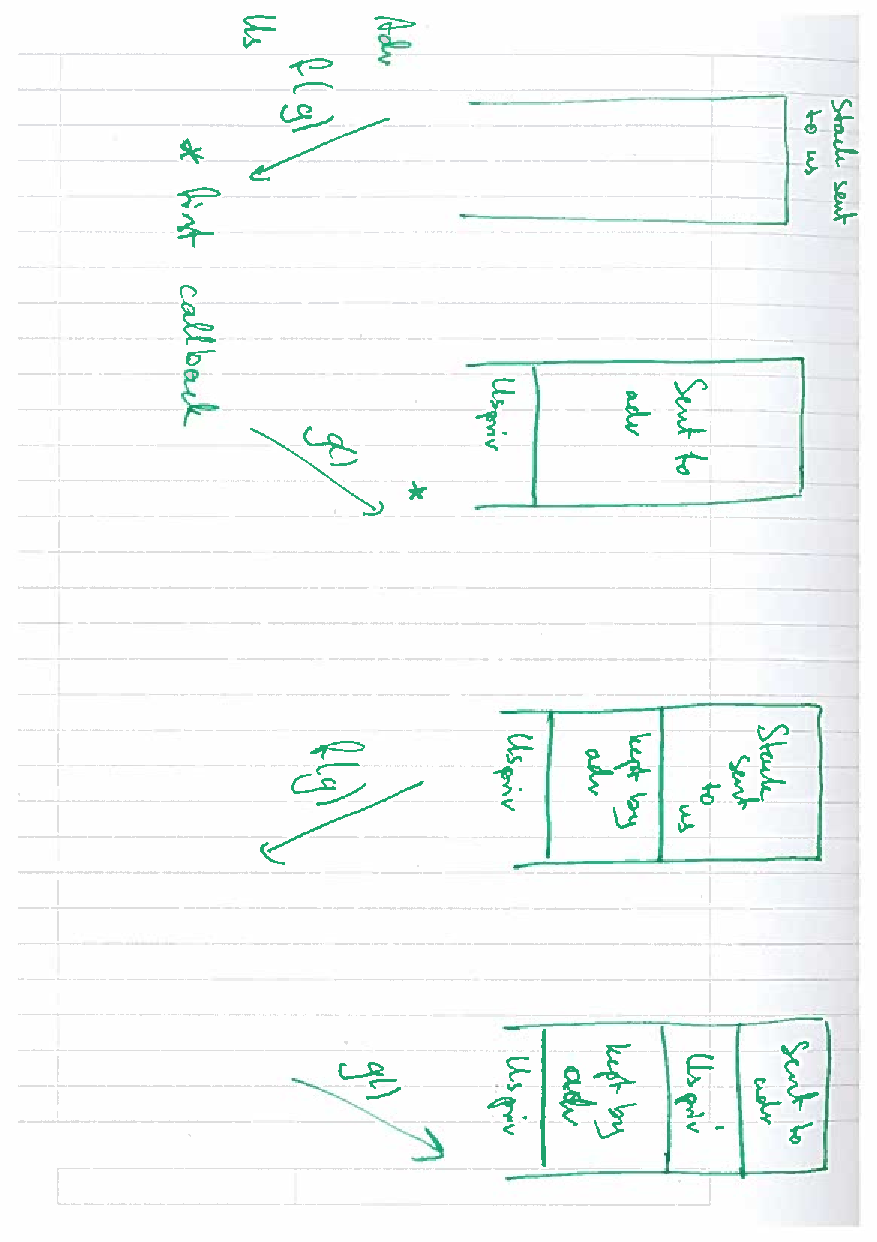
\includegraphics[angle=90,width=\textwidth]{img/ret-full-stk.pdf}
  \caption{Illustration of the stack in the example that illustrates why the entire stack must be returned.}
  \label{fig:ret-full-stk}
\end{figure}

\subsubsection{Restriction on stack allocation}
We need to somehow make sure that it is always the same stack that is used. If we don't, then an adversary can simply split the stack in two, use one part for one call and the other for another call. At this point, they can return to either of the two calls - in other words, well-bracketedness is not enforced.

\begin{itemize}
  \item An adversary starts the execution. They split the stack in two and call us with one part (say the top part) along with a callback.
  \item We use part of the stack and call the adversary with the rest of the stack.
  \item The adversary calls us again this time using the other part of the stack (here the bottom part of the stack).
  \item Again, we use part of the stack and call the adversary with the rest of this part of the stack.
\end{itemize}
At this point, the adversary can return from either of the two calls. Swapping around the order in which the adversary uses the two parts of the stack changes nothing.

The example is illustrated in Figure~\ref{fig:stk-alloc}.

One way to solve this problem is to make the "top address" of the stack known. There are many ways to do this, but we have chosen to do the following:
\begin{itemize}
\item The stack grows downwards, so the ``last address'' of the stack is the base address of the initial stack capability.
\item The base address of the stack capability is a fixed address, so in the semantics, it will be expressed as a constant that is publicly known.
\item At some point before a call, it must be checked whether the stack we are using actually has the globally known base address (if not we must fail because we cannot trust this stack).
\item To ensure that the check is made, we require it in the semantic condition (at this moment of time not defined, so we are yet to see what it looks like).
\end{itemize}

\begin{figure}
  \centering
  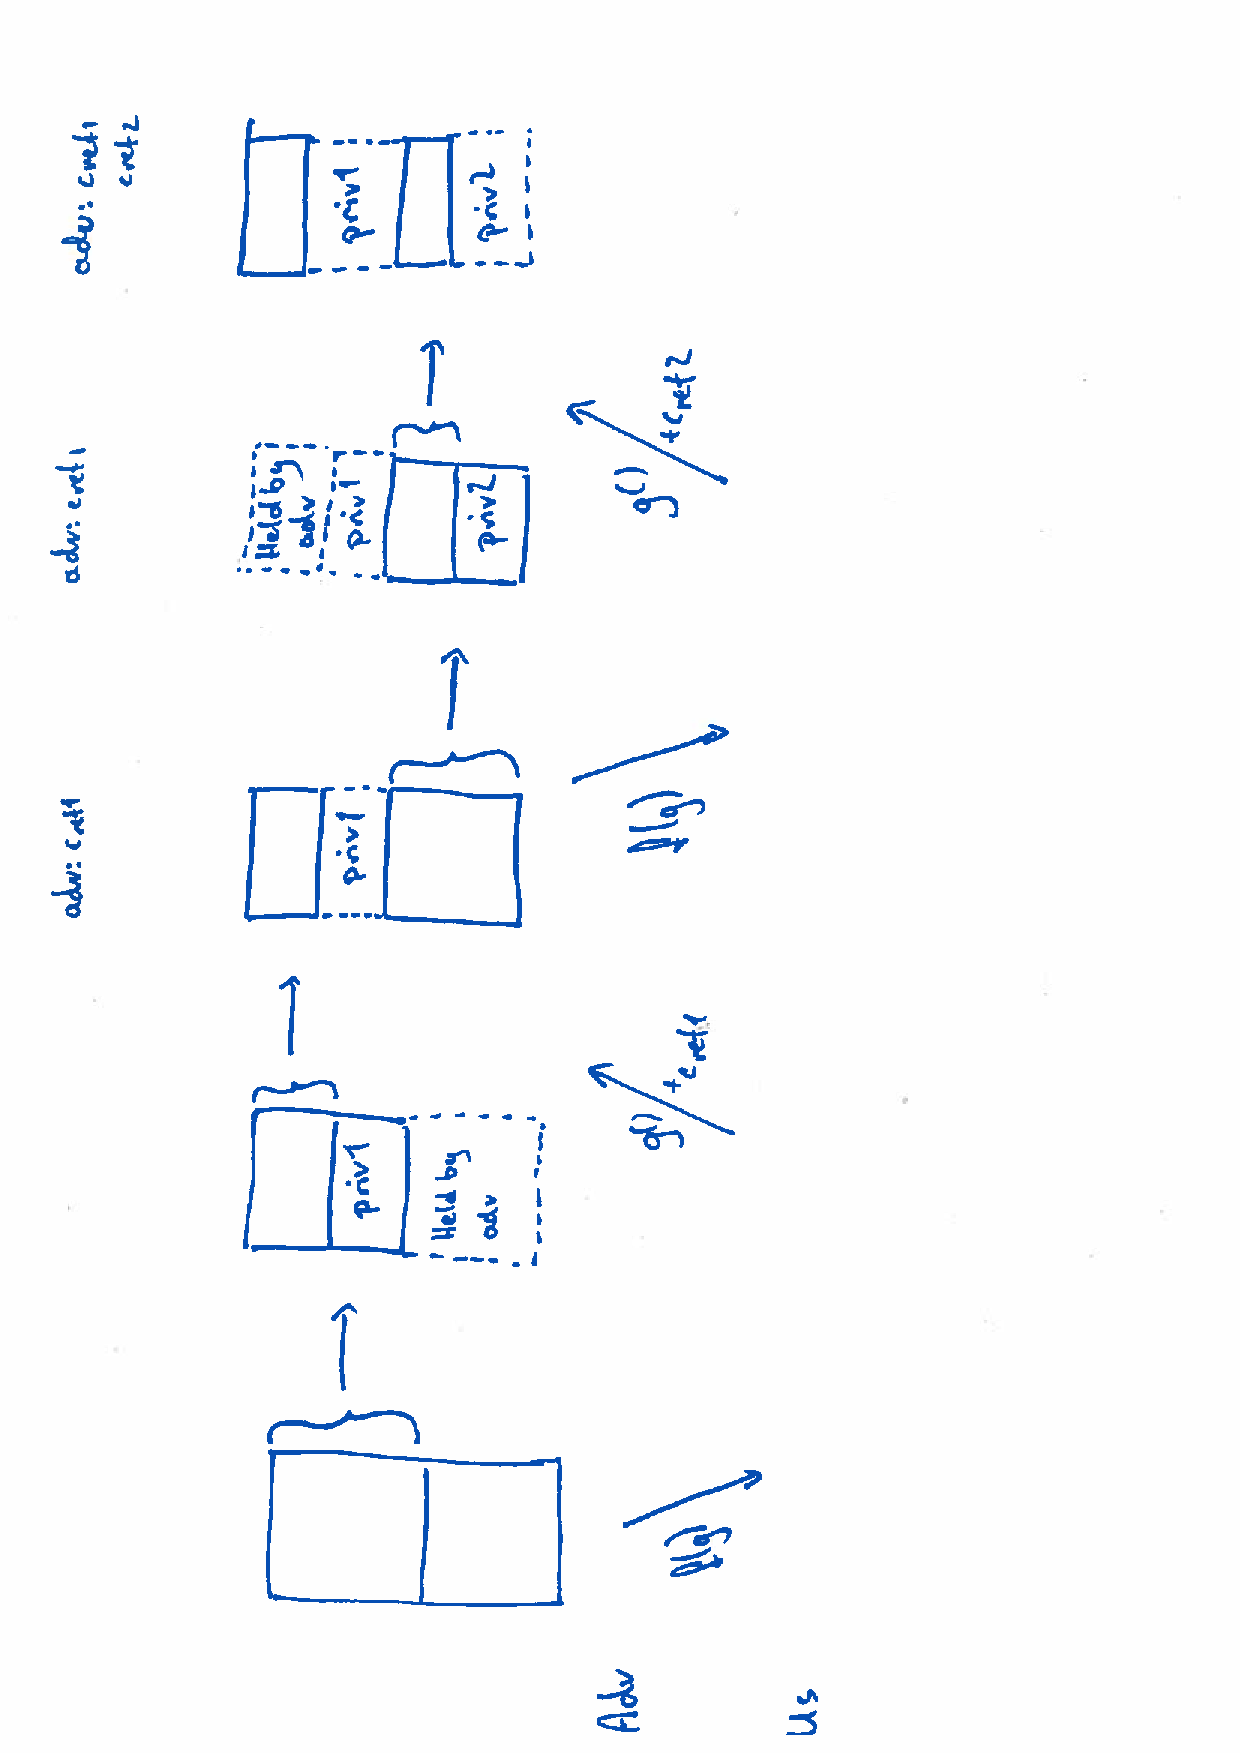
\includegraphics[angle=270,trim={0 0 5cm 0},width=\textwidth]{img/stk-alloc.pdf}
  \caption{Illustration of the potential stack allocation issue.}
  \label{fig:stk-alloc}
\end{figure}



\section{Related Work}
\subsection{Conditional Full-Abstraction}
The idea of conditional full-abstraction was used by \citet{Juglaret2016} to define full abstraction for unsafe languages. Their definition requires both the programs and the context to be fully defined (i.e.\ not cause undefined behavior). If the programs are not required to be fully-defined, then anything can happen which makes it impossible to reason about.. In our work, undefined behavior marks cases that we do not want to consider because they should be excluded further up in the compilation chain. Further, if we have to take these cases into account, then we need to add checks which protects the trusted code against itself, but properly compiled code should not have to protect itself against itself.
\lau{03-10-2017: We can adjust this when we have actually done something.}

Update: followup paper to the above presented at PriSC 2018, perhaps published elsewhere?
\url{https://popl18.sigplan.org/event/prisc-2018-formally-secure-compilation-of-unsafe-low-level-components}

\bibliography{references}
\end{document}